% =====================================================================================
%  Fusión de imágenes infrarrojas y visibles mediante morfología matemática
%  Tesis de Maestría en Ciencia de Datos, Universidad Comunera (UCOM)
%
%  Compilación:  latexmk -pdf main.tex     (o pdflatex → biber → pdflatex ×2)
% =====================================================================================
\documentclass[12pt,a4paper,oneside]{book}

% ---------- idioma y codificación -----------------------------------------------------
\usepackage[utf8]{inputenc}
\usepackage[T1]{fontenc}
% spanish, último de la lista, es el idioma principal; english solo silabea el Abstract.
% es-nodecimaldot es necesaria: sin ella babel-spanish imprime con coma los decimales en modo matemático.
\usepackage[english,es-tabla,es-nodecimaldot,spanish]{babel}
% Cortes de palabras inglesas de las referencias que el silabeo español hace mal.
\babelhyphenation[spanish]{multi-scale learn-ing Spring-er Py-Wave-lets}
\usepackage{lmodern}          % Latin Modern en todo el documento, también en la portada

% ---------- geometría e interlineado --------------------------------------------------
\usepackage[a4paper,left=25mm,right=25mm,top=25mm,bottom=25mm]{geometry}
\usepackage{setspace}
\onehalfspacing               % interlineado 1.5
\widowpenalty=10000           % sin líneas viudas
\clubpenalty=10000            % sin líneas huérfanas

% ---------- párrafos ------------------------------------------------------------------
\setlength{\parindent}{1.5em} % sangría de primera línea
\setlength{\parskip}{0pt}     % sin espacio extra entre párrafos

% ---------- pie de página: solo el número, centrado -----------------------------------
\usepackage{fancyhdr}
\pagestyle{fancy}
\fancyhf{}
\fancyfoot[C]{\thepage}
\renewcommand{\headrulewidth}{0pt}
\fancypagestyle{plain}{\fancyhf{}\fancyfoot[C]{\thepage}\renewcommand{\headrulewidth}{0pt}}

% ---------- títulos -------------------------------------------------------------------
% nobottomtitles*: un título que no deja debajo lugar para tres renglones pasa a la página siguiente.
% Se suma \pageshrink porque titlesec compara contra la página ya encogida.
\usepackage[nobottomtitles*]{titlesec}
\renewcommand{\bottomtitlespace}{\dimexpr5\baselineskip+\pageshrink\relax}
% Sin asterisco en \titlespacing, para que el primer párrafo del capítulo conserve la sangría.
\titleformat{\chapter}[display]
  {\normalfont\huge\bfseries}{\chaptertitlename\ \thechapter}{20pt}{\Huge}
\titlespacing{\chapter}{0pt}{50pt}{40pt}
% El punto final del número va en el formato y no en \thesection, para que \ref no lo repita.
\titleformat{\section}{\normalfont\Large\bfseries}{\thesection.}{1em}{}
\titleformat{\subsection}{\normalfont\large\bfseries}{\thesubsection.}{1em}{}

% ---------- tablas y figuras ----------------------------------------------------------
\usepackage{graphicx}
\usepackage{booktabs}
\usepackage{array}            % columnas con alineación propia (lista de abreviaturas)
\usepackage{longtable}        % la lista de abreviaturas ocupa más de una página
\usepackage{caption}
% Tablas: «Tabla N.M: Título» arriba, centrado, en el cuerpo del texto (12 pt).
\captionsetup{labelsep=colon}
\captionsetup[table]{position=above}
% Figuras: «Figura N.M» en negrita en su renglón y el título en cursiva debajo, arriba de la imagen.
\captionsetup[figure]{position=above,font=normalsize,labelfont=bf,textfont=it,labelsep=newline,justification=raggedright,singlelinecheck=false}
% Nota debajo de figuras y tablas, en \small y con «Nota.» en cursiva. Uso: \nota{Elaboración propia.}
\newcommand{\nota}[1]{\par\vspace{6pt}{\raggedright\small\textit{Nota.}\ #1\par}}
\usepackage[section]{placeins}
% En las páginas que solo tienen flotantes, estos van arriba y separados por el espacio normal.
\makeatletter
\setlength{\@fptop}{0pt}
\setlength{\@fpsep}{\floatsep}
\makeatother

% ---------- matemática ----------------------------------------------------------------
\usepackage{amsmath,amssymb}

% ---------- bibliografía APA ----------------------------------------------------------
% biblatex-apa requiere csquotes; autostyle toma las comillas del idioma activo de babel.
\usepackage[autostyle]{csquotes}
\usepackage[style=apa,backend=biber,natbib=true]{biblatex}
\DeclareLanguageMapping{spanish}{spanish-apa}
\addbibresource{referencias.bib}
% spanish.lbx pone guion en los rangos de páginas y quita la coma antes de «&» en las listas de
% tres o más nombres, como los editores. APA 7 usa raya corta y esa coma.
\DefineBibliographyExtras{spanish}{%
  \protected\def\bibrangedash{\textendash\penalty\hyphenpenalty}%
  \def\finalandcomma{\addcomma}}
% Las URL no se estiran entre caracteres y se pueden cortar también tras letras y cifras.
% \biburlbigskip es un registro muskip: va en mu, no en pt.
\biburlbigskip=0mu\relax
\setcounter{biburlnumpenalty}{9000}
\setcounter{biburlucpenalty}{8000}
\setcounter{biburllcpenalty}{7000}

% ---------- enlaces -------------------------------------------------------------------
\usepackage[hidelinks]{hyperref}

% ---------- datos del trabajo ---------------------------------------------------------
\newcommand{\titulotesis}{Fusión de imágenes infrarrojas y visibles mediante morfología matemática}
\newcommand{\subtitulotesis}{Un operador Top-Hat de una sola escala con un banco de cinco elementos
estructurantes: calidad de la fusión y aplicación a la detección de objetos}
\newcommand{\facultad}{Facultad de Informática}
\newcommand{\programa}{Maestría en Ciencia de Datos}
\newcommand{\autorA}{Juan Pablo Bazán}
\newcommand{\autorB}{Yan Bajac}
% \autores separa los nombres con \quad: sirve solo para la carátula, donde van solos en su renglón.
\newcommand{\autores}{Lic. \autorA{} \quad Ing. \autorB}
\newcommand{\tutor}{D.Sc. Julio César Mello}
\newcommand{\fechaentrega}{Diciembre 2026}
% Metadatos del PDF. Van después de los datos del trabajo, porque se expanden en el momento.
\hypersetup{pdftitle={\titulotesis}, pdfauthor={\autorA{} y \autorB},
  pdfsubject={Tesis de \programa, Universidad Comunera}, pdflang={es}}

% =====================================================================================
\begin{document}

% ---------- portada --------------------------------------------------------------------
% La portada no lleva ancla de página para no duplicar la del capítulo 1.
\hypersetup{pageanchor=false}
\begin{titlepage}
\centering

\includegraphics[width=50mm]{figuras/logo_ucom}\par
\vspace{1cm}
{\large \facultad\par}
\vspace{2cm}
{\huge\bfseries \titulotesis\par}
\vspace{2.8cm}
{\large Tesis para optar al título de \programa\par}
\vspace{0.5cm}
{\large Autores: \autorA{} y \autorB\par
Tutor: \tutor\par}
\vfill
{\large Asunción, Paraguay\par
\fechaentrega\par}
\end{titlepage}
\hypersetup{pageanchor=true}

% Los números romanos empiezan después de la portada: la carátula es la página i.
\frontmatter

% ---------- carátula -------------------------------------------------------------------
\thispagestyle{empty}
\begin{center}
{\huge\bfseries \titulotesis\par}
\vspace{0.6cm}
{\Large \subtitulotesis\par}
\vspace{3cm}
\begin{minipage}{0.75\textwidth}\centering\large
Tesis presentada a la \facultad{} de la Universidad Comunera como requisito para optar al título
de \programa.
\end{minipage}\par
\vspace{3cm}
{\large \autores\par}
\vspace{1cm}
{\large Tutor: \tutor\par}
\vfill
{\large Universidad Comunera\par
Asunción, Paraguay\par}
\end{center}
\clearpage

% ---------- hoja de aprobación ---------------------------------------------------------
\thispagestyle{empty}
\begin{center}
{\huge\bfseries \titulotesis\par}
\vspace{2cm}
\begin{minipage}{0.75\textwidth}\centering\large
Tesis presentada por Lic.~\mbox{\autorA} e \mbox{Ing.~\autorB} a la \facultad{} de la Universidad Comunera
como requisito para optar al título de \programa, y aprobada por el siguiente Tribunal Examinador.
\end{minipage}\par
\vspace{2.5cm}
\newcommand{\firma}{\rule{0.55\textwidth}{0.4pt}\par\vspace{0.2cm}{\large Nombre y firma\par}\vspace{1.6cm}}
\firma\firma\firma
{\large Fecha de aprobación: \rule{0.3\textwidth}{0.4pt}\par}
\end{center}
\clearpage

\chapter*{Resumen}
\phantomsection
\addcontentsline{toc}{chapter}{Resumen}

Se propone un algoritmo de fusión de imágenes infrarrojas y visibles basado en morfología matemática: un
Top-Hat de una sola escala con un disco y cuatro segmentos orientados. Suma al promedio de las dos imágenes
el detalle claro y le resta el oscuro, ambos multiplicados por un peso. Mediante optimización por enjambre
de partículas, el peso quedó en el mínimo permitido, 0.30, y se eligió el radio de 25 píxeles, que da más
realce. La hipótesis es que el algoritmo supera al Top-Hat clásico en calidad y en detectar objetos que ve
una sola cámara, y que es comparable en calidad a cinco métodos multiescala. Con seis métricas sin
referencia en veinte pares nocturnos, superó al Top-Hat clásico en cuatro, perdió en una y empató en otra.
Obtuvo el mejor rango promedio de los siete métodos, aunque por poco y con un orden que cambia según las
métricas: frente a los métodos multiescala, ganó contraste y nitidez y perdió parecido con las fuentes. En
otro conjunto, de día y de noche, la tasa de acierto equilibrada del detector entrenado con sus fusiones
fue del 61.4~\%. Promedia el acierto sobre los objetos que ve solo la cámara visible y sobre los que ve
solo la infrarroja. Esa tasa quedó cuarta entre ocho entradas fusionadas y 3.0 puntos por encima del Top-Hat
clásico, una ventaja mínima que cambió de signo según la semilla. En calidad la hipótesis se sostiene en lo
principal; en detección, queda por confirmar con nuevos entrenamientos y datos.

\textbf{Palabras clave:} Fusión de imágenes infrarrojas y visibles; Morfología matemática; Transformada
Top-Hat; Optimización por enjambre de partículas; Detección de objetos.

\chapter*{Abstract}
\phantomsection
\addcontentsline{toc}{chapter}{Abstract}

\begin{otherlanguage}{english}

An algorithm for fusing infrared and visible images based on mathematical morphology is proposed: a
single-scale Top-Hat with a disk and four oriented line segments. It adds the bright detail to the average
of the two images and subtracts the dark detail, both multiplied by a weight. Through particle swarm
optimization, the weight settled at the lowest allowed value, 0.30, and the radius of 25 pixels, which
gives more enhancement, was chosen. The hypothesis is that the algorithm outperforms the classical Top-Hat
in quality and in detecting objects seen by only one camera, and that it is comparable in quality to five
multiscale methods. With six no-reference metrics on twenty nighttime pairs, it outperformed the classical
Top-Hat on four, lost on one and tied on another. It achieved the best average rank of the seven methods,
though narrowly and with an order that changes with the metrics: against the multiscale methods, it gained
contrast and sharpness and lost similarity to the source images. On another dataset, with daytime and
nighttime scenes, the balanced hit rate of the detector trained on its fused images was 61.4\%. It averages the
hit rates on objects seen only by the visible camera and on those seen only by the infrared one. It ranked
fourth among eight fused inputs and was 3.0 points above the classical Top-Hat, a minimal advantage that
changed sign with the seed. The hypothesis largely holds for quality; for detection, it remains to be
confirmed with new training runs and data.

\textbf{Keywords:} Infrared and visible image fusion; Mathematical morphology; Top-Hat transform;
Particle swarm optimization; Object detection.

\end{otherlanguage}

\chapter*{Agradecimientos}
\phantomsection
\addcontentsline{toc}{chapter}{Agradecimientos}

A nuestras familias, por la paciencia y el apoyo de todos estos meses, en los que la tesis ocupó muchas
noches y fines de semana que también eran suyos.

Al \tutor, nuestro tutor, por su guía a lo largo de todo el trabajo y por sus observaciones, que nos
llevaron a revisar más de una vez lo que creíamos terminado.

A J. L. Vázquez Noguera y a H. Legal-Ayala, coautores del artículo sobre la fusión con la transformada
Top-Hat del que parte esta tesis.

A la Facultad de Informática de la Universidad Comunera y a los docentes de la Maestría en Ciencia de
Datos, por la formación recibida, y a nuestros compañeros de la maestría, por las discusiones y la ayuda
de cada semana.

Por último, a los autores de las colecciones de imágenes TNO y M3FD, que las pusieron a disposición de
todos y permitieron hacer este trabajo con datos públicos.


\tableofcontents
\chapter*{Lista de Abreviaturas y Símbolos}
\phantomsection
\addcontentsline{toc}{chapter}{Lista de Abreviaturas y Símbolos}

% Una sola lista, sin subtítulos, primero las siglas y después los símbolos. La sigla va alineada a
% la derecha en una columna de unos 27 mm, y el original en inglés, en cursiva entre paréntesis. Es una longtable porque la lista no entra en una sola página y una tabular no se corta.
{\setlength{\LTleft}{0pt}\setlength{\LTpre}{0pt}
\begin{longtable}{@{}>{\raggedleft\arraybackslash}p{0.17\textwidth}p{0.77\textwidth}@{}}
AP     & Precisión media (\textit{Average Precision}) \\
AP50   & Precisión media con un umbral de superposición (IoU) de 0.5 \\
BTH    & Transformada Top-Hat negra (\textit{Black Top-Hat}) \\
db4    & Base \textit{wavelet} de Daubechies de orden cuatro \\
DTCWT  & Transformada \textit{wavelet} compleja de doble árbol (\textit{Dual-Tree Complex Wavelet Transform}) \\
DWT    & Transformada \textit{wavelet} discreta (\textit{Discrete Wavelet Transform}) \\
EN     & Entropía (\textit{Entropy}) \\
FE     & Eficiencia de fusión (\textit{Fusion Efficiency}) \\
FMI    & Información mutua de características (\textit{Feature Mutual Information}) \\
IC     & Intervalo de confianza \\
IoU    & Intersección sobre la unión (\textit{Intersection over Union}) \\
IR     & Imagen infrarroja térmica (\textit{Infrared}) \\
JPEG   & Formato de compresión de imágenes (\textit{Joint Photographic Experts Group}) \\
M3FD   & Conjunto de pares de imágenes visibles e infrarrojas de varios escenarios, con objetos marcados (\textit{Multi-scenario Multi-modality Dataset}) \\
mAP50  & Media de la AP50 sobre las clases de objetos (\textit{mean Average Precision}) \\
MG     & Gradiente medio (\textit{Mean Gradient}) \\
MI     & Información mutua (\textit{Mutual Information}) \\
MSE    & Error cuadrático medio (\textit{Mean Squared Error}) \\
Nabf   & Medida del ruido y los artefactos que agrega la fusión \\
PASCAL VOC & Desafío de reconocimiento visual de objetos (\textit{Pattern Analysis, Statistical Modelling and Computational Learning Visual Object Classes}) \\
PSNR   & Relación señal-ruido de pico (\textit{Peak Signal-to-Noise Ratio}) \\
PSO    & Optimización por enjambre de partículas (\textit{Particle Swarm Optimization}) \\
Q0, QW, QE & Índices de calidad de Piella: ponderado por la varianza local, ponderado por ventana y de bordes \\
Qabf   & Índice que mide cuánta información de bordes pasa de las fuentes a la fusión \\
SCD    & Suma de las correlaciones de las diferencias (\textit{Sum of the Correlations of Differences}) \\
SD     & Desviación estándar (\textit{Standard Deviation}) \\
SF     & Frecuencia espacial (\textit{Spatial Frequency}) \\
SSIM   & Índice de similitud estructural (\textit{Structural Similarity}) \\
TNO    & Organización neerlandesa de investigación científica aplicada (\textit{Nederlandse Organisatie voor Toegepast Natuurwetenschappelijk Onderzoek}) \\
VIF    & Fidelidad de la información visual (\textit{Visual Information Fidelity}) \\
VIS    & Imagen visible (\textit{Visible}) \\
WTH    & Transformada Top-Hat blanca (\textit{White Top-Hat}) \\
YOLO   & Detector de objetos de una sola pasada (\textit{You Only Look Once}) \\
YOLOv8 & Octava versión de YOLO \\
YOLOv8n & Variante más pequeña (\textit{nano}) de YOLOv8 \\
$H$, $W$ & Número de filas y de columnas de una imagen \\
$f$    & Cualquier imagen normalizada \\
$I_{\mathrm{VIS}}$, $I_{\mathrm{IR}}$ & Imágenes fuente visible e infrarroja, normalizadas entre cero y uno \\
$F$    & Imagen fusionada \\
$b$    & Elemento estructurante \\
$\varepsilon$, $\delta$ & Erosión y dilatación \\
$\gamma$, $\varphi$ & Apertura y cierre \\
$r$    & Radio de los elementos estructurantes, en píxeles \\
$D_r$  & Disco de radio $r$ \\
$S_{r,\theta}$ & Segmento de radio $r$ y orientación $\theta$ \\
$m$    & Peso del detalle agregado en la regla de fusión \\
$\mathit{VP}$, $\mathit{FP}$, $\mathit{FN}$ & Verdaderos positivos, falsos positivos y falsos negativos de un detector \\
$P$, $R$ & Precisión y exhaustividad de un detector \\
\end{longtable}
\addtocounter{table}{-1}}

% Las dos listas entran al Índice general.
\clearpage\phantomsection\addcontentsline{toc}{chapter}{\listfigurename}
\listoffigures
\clearpage\phantomsection\addcontentsline{toc}{chapter}{\listtablename}
\listoftables

% ---------- cuerpo --------------------------------------------------------------------
\mainmatter

\chapter{Introducción}
\label{cap:introduccion}

Una misma escena se ve de manera diferente según la cámara que la observe. La cámara común forma la
imagen con la luz que reflejan las superficies; por eso recoge el color y la textura. La cámara térmica
mide, en cambio, la radiación infrarroja que emite cada cuerpo según su temperatura. Gracias a eso, una
persona o un vehículo con el motor caliente resaltan sobre el fondo aun de noche o entre el humo. A
cambio, la imagen térmica pierde buena parte de esa textura. Ninguna de las dos cámaras basta por sí
sola en todas las condiciones. La fusión de imágenes infrarrojas y visibles combina ambas fuentes en una
sola imagen que conserve lo útil de cada una \parencite{ma2019}.

La Figura~\ref{fig:modalidades} muestra una escena nocturna en sus dos imágenes, la visible y la
infrarroja, junto con la que resulta de fusionarlas con el algoritmo que propone este trabajo. En la
imagen visible se distinguen los arbustos, el empedrado y la entrada del edificio, pero la persona que
camina junto a la entrada se confunde con los arbustos que tiene detrás. En la infrarroja, la persona
resalta en blanco, mientras el follaje queda oscuro y casi sin textura. La imagen fusionada conserva a la
vez la figura de la persona y la textura del fondo.

\begin{figure}[htbp]
\centering
\caption{Escena nocturna en la imagen visible, en la infrarroja y fusionada con el algoritmo propuesto}
\label{fig:modalidades}
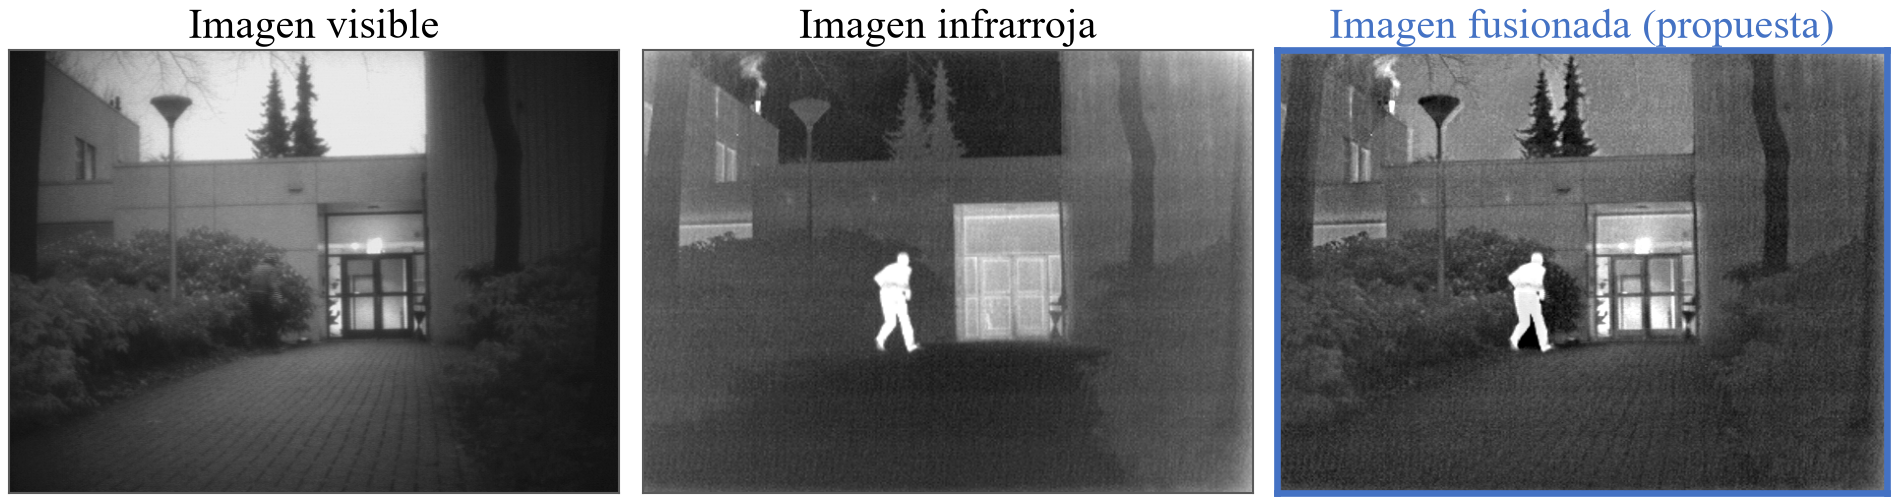
\includegraphics[width=\textwidth]{figuras/fig_modalidades}
\nota{Elaboración propia a partir de imágenes del conjunto de \textcite{toet2014, toet2017}. La escena
corresponde al par Kaptein 1123, uno de los veinte con que se evalúa la calidad
(Sección~\ref{sec:corpus}). La imagen fusionada, recuadrada a la derecha, se obtuvo con la configuración
adoptada, radio $r = 25$ y peso $m = 0.30$ (Sección~\ref{sec:ajuste}). La
Figura~\ref{fig:montaje_kaptein} muestra la misma escena fusionada con los demás métodos del estudio.}
\end{figure}

Los métodos de fusión se agrupan en varias familias \parencite{li2017, singh2023}. Los multiescala, como
las pirámides y las transformadas \textit{wavelet}, descomponen cada fuente en capas según el tamaño
del detalle, combinan las capas y reconstruyen la imagen. Otros recurren a representaciones dispersas,
que describen cada región con pocos elementos de un diccionario. Los más recientes emplean redes
neuronales que aprenden la regla de fusión a partir de ejemplos. La morfología matemática ofrece un
camino distinto.
Sus operadores recorren la imagen con una forma pequeña, el elemento estructurante, y la transforman
según cómo esa forma encaja en cada región. Con ellos, la transformada Top-Hat separa del fondo los
detalles claros u oscuros más pequeños que el elemento \parencite{soille2003, gonzalez2018}. Esa
separación ya se aprovechó para fusionar imágenes infrarrojas y visibles \parencite{bai2013, roman2020,
bajacfigueredo2024}.

Este trabajo propone un algoritmo de fusión de imágenes infrarrojas y visibles basado en morfología
matemática. Su núcleo es un operador Top-Hat de una sola escala. En lugar de un único elemento
estructurante, emplea un banco de cinco: un disco y cuatro segmentos lineales orientados a $0^\circ$,
$45^\circ$, $90^\circ$ y $135^\circ$. El detalle de cada fuente es la suma de lo que extrae el disco
y el promedio de lo que extraen los cuatro segmentos. La regla de fusión parte del promedio de las
dos fuentes, le suma el detalle claro y le resta el oscuro. Un peso $m$ regula cuánto detalle se agrega.
El algoritmo queda así definido por dos parámetros: el radio $r$ de los elementos y el peso $m$. Ambos se
ajustan mediante optimización por enjambre de partículas. En esa búsqueda, un grupo de soluciones
candidatas recorre el espacio de los parámetros, guiado por las mejores posiciones halladas. En las
veinticinco corridas del enjambre, el peso terminó en 0.30, que es el límite inferior del rango de búsqueda. El
radio quedó casi siempre en 1 o en 25 píxeles. De esos dos valores se adoptó $r = 25$, porque prioriza
el realce: da más contraste y nitidez que $r = 1$, a cambio de una imagen menos fiel a las fuentes.

El problema que aborda la tesis tiene dos partes. La primera se refiere a la calidad: si las imágenes del
algoritmo propuesto están a la altura de las que producen los métodos clásicos de fusión. Como
referencia se toman el Top-Hat clásico, que aplica la misma regla con un único disco, y cinco métodos
multiescala: dos pirámides y tres transformadas \textit{wavelet}. La segunda parte es la aplicación: si
esas imágenes ayudan a un detector automático a encontrar objetos. La variable que se manipula es el
método de fusión; las que se miden son la calidad de la imagen y el acierto del detector.

Medir la calidad tiene una dificultad propia, porque no existe una imagen fusionada ideal con la cual
comparar. Por eso se recurre a métricas sin referencia, que prescinden de ella pero no siempre coinciden
entre sí. El trabajo de \textcite{bajacfigueredo2024}, en el que participaron los
autores de esta tesis, ilustra ese desacuerdo. En la escena Camp, con elementos estructurantes de tamaños
7 y 9, la fusión con Top-Hat de ese trabajo quedó primera en desviación estándar, entropía y frecuencia
espacial, que miden el contraste, la información y la nitidez. Al mismo tiempo quedó última en
información mutua, que mide el parecido con las fuentes.

La propuesta reúne piezas que provienen de trabajos distintos. El banco de cinco elementos
estructurantes se diseñó para realzar el contraste local y la nitidez en mamografías \parencite{floressf}.
La forma de combinar las respuestas del disco y de los segmentos se tomó de un método de realce de
imágenes de fondo de ojo \parencite{bala2024}. La regla de fusión con un peso y el ajuste del radio y del
peso por enjambre de partículas provienen de \textcite{ortegarodriguez2025}, que trabajaron con un único
disco. El Top-Hat clásico sigue la fusión con Top-Hat del trabajo ya citado
\parencite{bajacfigueredo2024} y se aplica aquí con un disco de radio 5 y peso 1. En la literatura
revisada no se encontró el banco aplicado a la fusión de imágenes infrarrojas y visibles. El aporte de
la tesis es llevarlo a esa fusión, junto con el ajuste de sus parámetros. Sobre esa base se
caracteriza la calidad de las imágenes resultantes y se evalúa la aplicación del algoritmo a la
detección. A diferencia
de una red neuronal, un operador morfológico puede explicarse paso a paso. Esa transparencia permite relacionar lo que premia cada métrica con lo
que hace la regla de fusión.

Las métricas de imagen dicen poco sobre lo que la fusión aporta a un uso concreto. Por eso, trabajos
recientes la evalúan también por su efecto en una tarea posterior, como la detección o la segmentación
de objetos \parencite{liu2022, tang2022}. Un detector que recibe la imagen fusionada debería encontrar
en ella lo que cada cámara muestra por separado. Un peatón en la sombra y un farol encendido ilustran el
caso. Al primero lo ve casi solo la cámara térmica; al segundo, casi solo la común. En la aplicación, la
propuesta se compara con el Top-Hat clásico, que pertenece a la misma familia y usa la misma regla.
Así, la comparación mide el efecto de cambiar el operador en su conjunto, con sus elementos
estructurantes, su radio y su peso.

Se plantean, en consecuencia, dos preguntas de investigación, una sobre la calidad de la fusión y otra
sobre su aplicación. ¿Qué calidad tienen las imágenes del algoritmo propuesto, frente al Top-Hat clásico
y a cinco métodos multiescala? ¿Encuentra un detector entrenado con esas imágenes más objetos vistos por
una sola cámara que uno entrenado con las del Top-Hat clásico?

La hipótesis del trabajo es la siguiente.

El algoritmo de fusión propuesto, con sus parámetros ajustados mediante optimización por enjambre de
partículas, produce imágenes de mejor calidad que el Top-Hat clásico y de calidad comparable a la de
cinco métodos multiescala, medida con seis métricas sin referencia. En su aplicación a la detección de
objetos, un detector entrenado con sus imágenes encuentra más objetos vistos por una sola cámara que el
entrenado con las imágenes del Top-Hat clásico.

Las dos oraciones de la hipótesis reúnen tres afirmaciones: dos sobre la calidad (frente al Top-Hat
clásico y frente a los métodos multiescala) y una sobre la aplicación a la detección. Cada una se examina
con las pruebas de la evaluación que le corresponde, sin agregar otras (Sección~\ref{sec:examen-hipotesis}).

El trabajo se sitúa en el año 2026 y se desarrolló en el marco de la Maestría en Ciencia de Datos de la
Universidad Comunera. Sus beneficiarios son, en primer lugar, los investigadores en procesamiento de
imágenes, que disponen de un operador morfológico descrito paso a paso y comparado con métodos
establecidos. También lo son quienes desarrollan sistemas de vigilancia o de detección con cámaras
visibles y térmicas y deben decidir cómo fusionar sus imágenes.

\section{Objetivos del trabajo}
\label{sec:objetivos}

\subsection{Objetivo general}

Proponer un algoritmo de fusión de imágenes infrarrojas y visibles basado en morfología matemática, con
sus parámetros ajustados mediante optimización por enjambre de partículas, y evaluar la calidad de sus
imágenes y su aplicación a la detección de objetos.

\subsection{Objetivos específicos}

Para alcanzar el objetivo general se plantean cuatro objetivos específicos. Las conclusiones del
Capítulo~\ref{cap:conclusiones} los retoman en el mismo orden.

\begin{itemize}
\item Implementar el algoritmo propuesto y ajustar su radio y su peso mediante optimización por enjambre
de partículas.
\item Evaluar la calidad de sus imágenes con seis métricas sin referencia y pruebas estadísticas no
paramétricas, frente al Top-Hat clásico y a cinco métodos multiescala.
\item Evaluar su aplicación a la detección de objetos vistos por una sola cámara, frente al Top-Hat
clásico, con detectores entrenados sobre cada tipo de imagen.
\item Examinar la hipótesis con los resultados de las dos evaluaciones.
\end{itemize}

\section{Alcance y delimitaciones}
\label{sec:limitaciones}

Los resultados del estudio deben leerse dentro de los límites siguientes:

\begin{itemize}
\item \textbf{Validez interna:} Las métricas sin referencia premian propiedades distintas de la imagen,
de modo que el orden entre los métodos depende del conjunto de métricas elegido. Los métodos
comparativos se aplican con sus parámetros por defecto, sin ajuste. En cambio, la aptitud del enjambre
se calculó sobre tres de los veinte pares con que se evalúa la calidad, y el radio se eligió entre los
dos que dio el enjambre comparándolos sobre los veinte.
\item \textbf{Detección:} Los detectores entrenados con cada cámara, y no una revisión humana, definen
cuáles son los objetos vistos por una sola cámara. Los objetos de la prueba provienen de pocos tramos de video, y casi dos
de cada tres luces salen de un mismo grupo de tramos. Se emplea un solo modelo de detector, el más
pequeño de su familia, entrenado durante cuarenta épocas (pasadas completas por los datos de
entrenamiento).
\item \textbf{Validez externa:} La calidad se mide en veinte pares de un único conjunto, el
\textit{TNO Image Fusion Dataset} \parencite{toet2014, toet2017}. TNO es la sigla de la organización neerlandesa
de investigación científica aplicada (del neerlandés \textit{Nederlandse Organisatie voor Toegepast
Natuurwetenschappelijk Onderzoek}), que reunió las imágenes. En buena parte de esos pares, la imagen
visible proviene de cámaras con intensificador de imagen, que amplifican la escasa luz disponible. La
detección se evalúa en otro conjunto, M3FD (del inglés \textit{Multi-scenario Multi-modality
Dataset}), con pares de escenas diurnas y nocturnas en los que los objetos están marcados
\parencite{liu2022}. De sus seis clases de objetos, el análisis se centra en dos, las personas y las
luces. La imagen visible se usa en escala de grises. El radio se expresa en píxeles y no se adapta al
tamaño de la imagen.
\item \textbf{Alcance:} El estudio usa solo conjuntos públicos, cuyos pares ya vienen registrados por sus
autores; el corrimiento vertical de varios píxeles que muestran algunos pares del TNO no se corrigió
(Sección~\ref{sec:corpus}). No incluye captura propia de imágenes, alineación de pares ni medición del tiempo de cómputo.
Su foco es un operador de una sola escala. Por eso quedan fuera, para trabajos futuros
(Capítulo~\ref{cap:recomendaciones}), la fusión con redes neuronales y los métodos morfológicos
multiescala de \textcite{bai2013} y \textcite{roman2020}.
\end{itemize}

\section{Estructura del documento}
\label{sec:estructura}

Después de esta introducción, el documento se organiza de la manera siguiente:

\begin{itemize}
\item El Capítulo~\ref{cap:marco} expone el marco teórico y conceptual. Parte de los conceptos básicos
sobre la imagen digital y la fusión. Trata después los métodos de fusión de imágenes visibles e
infrarrojas, la morfología matemática, las métricas sin referencia y las pruebas estadísticas. Siguen
la optimización por enjambre de partículas y la detección de objetos, y el capítulo
cierra con el estado del arte y la brecha existente.
\item El Capítulo~\ref{cap:metodologia} describe los conjuntos de imágenes, el algoritmo propuesto y el
ajuste de sus parámetros, las dos evaluaciones y el examen de la hipótesis.
\item El Capítulo~\ref{cap:resultados} presenta los resultados en ese mismo orden: la caracterización de
los conjuntos, el ajuste, la calidad de imagen con su análisis estadístico, la detección y el examen de
la hipótesis.
\item El Capítulo~\ref{cap:discusion} discute la calidad y su costo, el ajuste, la detección y la
relación entre ambas, y precisa las limitaciones del estudio.
\item El Capítulo~\ref{cap:conclusiones} presenta las conclusiones, una por cada objetivo específico.
\item El Capítulo~\ref{cap:recomendaciones} reúne las recomendaciones para trabajos futuros.
\item Los Anexos reúnen la participación de los autores en congresos y la tabla completa de los
contrastes de Wilcoxon (Tabla~\ref{tab:wilcoxon_completa}).
\end{itemize}

\chapter{Marco teórico y conceptual}
\label{cap:marco}

Este capítulo reúne los conceptos y los métodos en que se apoya el trabajo.

\section{Conceptos básicos}
\label{sec:conceptos}

\subsection{Imagen digital}

Una imagen digital en escala de grises, es decir, sin color, es una cuadrícula de $H$ filas y $W$
columnas de puntos llamados píxeles. Cada píxel guarda un número entero, su nivel de gris, que indica
cuán claro se ve ese punto \parencite{gonzalez2018}. En las imágenes de este trabajo, ese nivel va de 0,
el negro, a 255, el blanco. La fusión y las seis métricas que se usan aquí operan sobre la intensidad
normalizada, que lleva esos niveles al intervalo de cero a uno:
\begin{equation} f(x,y) = \frac{g(x,y)}{255}. \label{eq:intensidad} \end{equation}
En ella, $g(x,y)$ es el nivel de gris del píxel de la columna $x$ y la fila $y$, y $f(x,y)$ es su
intensidad normalizada. En adelante, la letra $f$ designa cualquier imagen normalizada.

\subsection{Imágenes visible e infrarroja}

La imagen visible (VIS) es la que toma una cámara común. Registra la luz que reflejan los objetos,
dentro de la franja que percibe el ojo humano. Por eso muestra bien la textura, los bordes y los
carteles, pero pierde calidad con poca luz o con mal tiempo. La imagen infrarroja térmica (IR) registra
en cambio el calor que emite cada cuerpo según su temperatura. Distingue a una persona o a un motor a
oscuras, aunque suele ofrecer menos detalle fino y poca textura \parencite{ma2019, bajacfigueredo2024}.
Aquí, la imagen visible en color se pasa a escala de grises antes de fusionarla.

Un par visible-infrarrojo está formado por dos imágenes de la misma escena, una de cada cámara, tomadas
al mismo tiempo. Para fusionarlas, las dos imágenes deben estar registradas, es decir, alineadas de modo
que un mismo píxel corresponda al mismo punto de la escena \parencite{gonzalez2018}. El registro corrige
las diferencias de posición, giro y tamaño que aparecen porque las cámaras no miran desde el mismo lugar.
Si el registro falla, el detalle de una imagen queda desplazado respecto del de la otra, y un borde puede
aparecer dos veces. Este trabajo no registra imágenes: usa conjuntos públicos cuyos pares ya vienen
registrados por sus autores.

\subsection{Niveles de fusión}

Las imágenes que se combinan se llaman fuentes. Según qué se combina, la fusión se clasifica en tres
niveles: de píxel, de características y de decisiones \parencite{singh2023}. El nivel de características
combina rasgos ya extraídos de cada fuente, como los bordes. El de decisiones combina los resultados de
sistemas que analizan cada fuente por separado, como dos detectores de objetos. El nivel de píxel
combina las fuentes punto por punto, sobre sus intensidades o sobre una versión transformada
\parencite{li2017}. Todos los métodos de este trabajo son de este último nivel. Su resultado
es una imagen del mismo tamaño que las fuentes:
\begin{equation} F = \Phi\left(I_{\mathrm{VIS}},\, I_{\mathrm{IR}}\right). \label{eq:fusion-pixel} \end{equation}
En ella, $I_{\mathrm{VIS}}$ e $I_{\mathrm{IR}}$ son las fuentes visible e infrarroja normalizadas, $\Phi$
es el método de fusión y $F$ es la imagen fusionada. Aquí $F$ también toma valores entre cero y uno,
porque todos los métodos recortan su resultado a ese intervalo.

\subsection{Evaluación sin imagen de referencia}

En la fusión de imágenes no siempre existe una imagen de referencia, es decir, una imagen fusionada
correcta con la cual comparar el resultado \parencite{singh2023}. En la fusión visible-infrarroja no existe,
porque ninguna cámara puede tomar la imagen ideal que reúna lo mejor de las dos. Por eso la calidad se
estima con métricas sin referencia, indicadores numéricos que no necesitan esa imagen. Unas se calculan
sobre la imagen fusionada sola y miden cuánta información, contraste o nitidez contiene. Otras la
comparan con cada fuente y miden cuánto conserva de la visible y de la infrarroja. Como cada métrica
premia una propiedad distinta, dos métricas pueden ordenar de manera diferente a los mismos métodos. La
Sección~\ref{sec:metricas} presenta las que se usan aquí.

\section{Fusión de imágenes visibles e infrarrojas}
\label{sec:fusion}

Cada cámara capta una parte de la escena y pierde otra. La fusión visible-infrarroja reúne en una sola
imagen la textura de la visible y el calor de la infrarroja \parencite{ma2019}. Sus usos van de la
vigilancia a la detección y el seguimiento de objetos \parencite{li2017, zhang2023}. Las revisiones del
área agrupan los métodos de fusión en varias familias \parencite{li2017, ma2019, singh2023}.

\subsection{Familias de métodos}

Una de las familias más difundidas es la multiescala \parencite{li2017}. Sus métodos descomponen cada
imagen en una base, con el brillo general, y en capas de detalle de distintos tamaños. Luego combinan
cada capa con su propia regla y reconstruyen el resultado. Son de este tipo las pirámides, que
representan la imagen a resoluciones cada vez menores, y las transformadas \textit{wavelet}, que la
analizan con ondas breves. También lo son los cinco métodos multiescala con que se compara la propuesta,
descritos en la Sección~\ref{sec:comparativos}.

Otra familia usa representaciones dispersas: cada bloque pequeño de la imagen se escribe como la suma de
pocos patrones tomados de un repertorio llamado diccionario, cada uno con su peso. En la fusión
visible-infrarroja, \textcite{wang2014} aplican esa idea sin admitir pesos negativos.

Una tercera familia usa redes neuronales, modelos que aprenden a fusionar a partir de ejemplos
\parencite{zhang2023}. FusionGAN, por ejemplo, enfrenta dos redes: una produce la imagen fusionada y la
otra la juzga. Así, la regla de fusión se aprende de los ejemplos en lugar de diseñarse a mano
\parencite{ma2019b}. Por eso, estos métodos necesitan entrenarse antes de usarse. Los métodos
morfológicos, en cambio, siguen pasos explícitos: extraen el detalle comparando la imagen con una figura
pequeña de forma conocida \parencite{serra1982}. La propuesta de este trabajo pertenece a este grupo.
Sus herramientas y su uso en la fusión se presentan en la Sección~\ref{sec:morfologia}.

\subsection{Métodos multiescala comparativos}
\label{sec:comparativos}

La propuesta se compara con cinco métodos multiescala y con el Top-Hat clásico, que se presenta en la
Sección~\ref{sec:fusion-tophat}. Los cinco multiescala separan cada imagen en capas de distinto detalle,
las combinan y reconstruyen la imagen fusionada. En los cinco métodos, el resultado se recorta al
intervalo de cero a uno.

\subsubsection{Pirámide de Laplace}

La pirámide de Laplace \parencite{burt1983} se propuso como método de codificación compacta de
imágenes. Usa copias $G_\ell$ cada vez más suaves y reducidas a la mitad, desde $G_0$, que es la imagen.
Cada capa $L_\ell$ guarda lo que se pierde al reducir. Con $K$ capas,
\begin{equation} L_\ell = G_\ell - \operatorname{amp}(G_{\ell+1}), \quad \ell = 0, 1, \ldots, K-2, \qquad L_{K-1} = G_{K-1}. \label{eq:laplace} \end{equation}
Aquí $\operatorname{amp}(\cdot)$ amplía una copia al doble y la suaviza. La capa fusionada $L^F_\ell$,
incluida la más gruesa, toma en cada píxel el valor de la fuente de mayor actividad local. Esa actividad
es el valor absoluto de la capa, suavizado en una ventana cuadrada que pesa más el centro. Para
reconstruir, se amplía $L^F_{K-1}$, se le suma $L^F_{K-2}$ y se repite el paso hasta $L^F_0$.

\subsubsection{Pirámide de razón}

La pirámide de razón de \textcite{toet1989}, pensada para la fusión, divide en lugar de restar. Con $K$
niveles usa $K+1$ de esas copias, de $G_0$ a $G_K$:
\begin{equation} R_\ell = \frac{G_\ell + \eta}{\operatorname{amp}(G_{\ell+1}) + \eta}, \qquad \ell = 0, 1, \ldots, K-1. \label{eq:razon} \end{equation}
La constante $\eta$ evita dividir por cero. Una razón igual a uno indica que no hay contraste local. Si
es mayor que uno, el punto es más claro que su entorno, y si es menor, más oscuro. En cada píxel, la
razón fusionada $R^F_\ell$ es la más alejada de uno, la de mayor contraste. La copia fusionada más
gruesa, $G^F_K$, es el promedio de las dos $G_K$. Desde ella se reconstruye por multiplicación:
\begin{equation} G^F_\ell = R^F_\ell \left[ \operatorname{amp}(G^F_{\ell+1}) + \eta \right], \qquad \ell = K-1, \ldots, 1, 0. \label{eq:razon-reconstruccion} \end{equation}
La imagen fusionada es $G^F_0$.

\subsubsection{Transformada \textit{wavelet} discreta}

La transformada \textit{wavelet} discreta (DWT, del inglés \textit{Discrete Wavelet Transform}) mide los
cambios de la imagen con una \textit{wavelet}, una onda breve usada como patrón. En cada nivel separa la
imagen en una aproximación suavizada, de alrededor de la mitad de ancho y alto, y tres detalles:
horizontal, vertical y diagonal \parencite{gonzalez2018}. El proceso se repite sobre la aproximación, y
cada valor obtenido es un coeficiente. El trabajo de \textcite{li1995} la aplica a la fusión de imágenes
de distintos sensores. La primera de las dos DWT comparadas, llamada DWT (Haar), usa la base de Haar. Esa base es la
onda más simple: suma y resta píxeles vecinos por pares \parencite{gonzalez2018}. La aproximación $A$ se
promedia. Cada coeficiente de detalle $D$ se toma de la fuente en que es mayor en valor absoluto:
\begin{equation} A^F=\tfrac{1}{2}\bigl(A^{\mathrm{VIS}}+A^{\mathrm{IR}}\bigr), \qquad D^F=\begin{cases} D^{\mathrm{VIS}} & \text{si } |D^{\mathrm{VIS}}|\geq|D^{\mathrm{IR}}|,\\ D^{\mathrm{IR}} & \text{en otro caso}. \end{cases} \label{eq:regla-wavelet} \end{equation}

\subsubsection{Transformada \textit{wavelet} compleja de doble árbol}

Según \textcite{kingsbury2001}, la DWT tiene dos límites: sus coeficientes cambian mucho si la imagen se
desplaza un píxel, y solo distingue tres direcciones. La transformada \textit{wavelet} compleja de doble
árbol (DTCWT, del inglés \textit{Dual-Tree Complex Wavelet Transform}) busca un análisis casi invariante
al desplazamiento, es decir, estable ante esos cambios. Usa dos cadenas de filtros en paralelo, llamadas
árboles; un filtro es una operación que deja pasar solo ciertos detalles. Las salidas de los
árboles forman coeficientes complejos, números con una parte real y otra imaginaria. El módulo de cada coeficiente, que
reúne las dos partes en un solo valor, varía poco ante desplazamientos pequeños. Cada nivel ofrece,
además, seis orientaciones. Para fusionar se aplica la regla de la Ecuación~\eqref{eq:regla-wavelet},
con el módulo en lugar del valor absoluto.

\subsubsection{Transformada \textit{wavelet} discreta con la base de Daubechies}

El quinto método multiescala es una segunda DWT, con la regla de la
Ecuación~\eqref{eq:regla-wavelet} y la base de Daubechies de orden cuatro \parencite{daubechies1988}. Esa base tiene filtros más
largos y una onda más suave que la de Haar. Como sigue siendo una DWT, distingue las mismas tres
direcciones. En adelante se la llama DWT (db4), para distinguirla de la DWT (Haar).

\section{Morfología matemática y transformada Top-Hat}
\label{sec:morfologia}

La morfología matemática analiza la forma de las estructuras de una imagen \parencite{serra1982}. Para
eso la compara con una figura pequeña de forma conocida, llamada elemento estructurante, que se desplaza
por todos los píxeles. En escala de grises, cada nivel de gris se lee como una altura, y la imagen se ve
como un relieve de montes claros y valles oscuros. El elemento estructurante $b$ es el conjunto de
desplazamientos $(j,k)$ de sus píxeles respecto de su centro, e incluye al centro mismo. El
desplazamiento $j$ se mide en columnas y $k$ en filas, como $x$ e $y$ en la imagen. La forma y el tamaño
del elemento deciden qué detalles se conservan.

\subsection{Operaciones básicas}

Las operaciones morfológicas parten de dos básicas, la erosión y la dilatación
\parencite{soille2003, gonzalez2018}. La erosión, $\varepsilon$, toma en cada píxel el menor nivel de
gris bajo el elemento centrado en él, y la dilatación, $\delta$, el mayor:
\begin{equation} \varepsilon(f,b)(x,y) = \min_{(j,k)\in b} f(x+j,\, y+k), \qquad \delta(f,b)(x,y) = \max_{(j,k)\in b} f(x+j,\, y+k). \label{eq:erosion-dilatacion} \end{equation}
Los vecinos que caen fuera de la imagen se ignoran. El elemento es plano: solo indica qué vecinos se
comparan. La erosión angosta los montes y borra los más estrechos que el elemento, y la dilatación hace
lo mismo con los valles. Algunos textos, como el de \textcite{gonzalez2018}, giran el elemento media
vuelta en la dilatación. Con elementos simétricos respecto de su centro, como los de este trabajo, ese
giro no cambia el resultado.

La apertura, $\gamma$, es una erosión seguida de una dilatación con el mismo elemento. El cierre,
$\varphi$, es una dilatación seguida de una erosión:
\begin{equation} \gamma(f,b) = \delta\bigl(\varepsilon(f,b),\, b\bigr), \qquad \varphi(f,b) = \varepsilon\bigl(\delta(f,b),\, b\bigr). \label{eq:apertura-cierre} \end{equation}
La apertura rebaja los montes en los que el elemento no cabe hasta la altura en que sí cabe, y deja casi
intacto el resto. El cierre rellena, del mismo modo, los valles en los que el elemento no cabe. Por eso
la apertura nunca supera a la imagen y el cierre nunca queda por debajo de ella \parencite{soille2003}.
La Figura~\ref{fig:morfologia} muestra el efecto de estas cuatro operaciones sobre una señal de una
dimensión, como los niveles de gris a lo largo de una fila. Su último panel anticipa la transformada
Top-Hat, que se define a continuación.

\begin{figure}[htbp]
\centering
\caption{Operaciones morfológicas básicas y transformada Top-Hat sobre una señal de una dimensión}
\label{fig:morfologia}
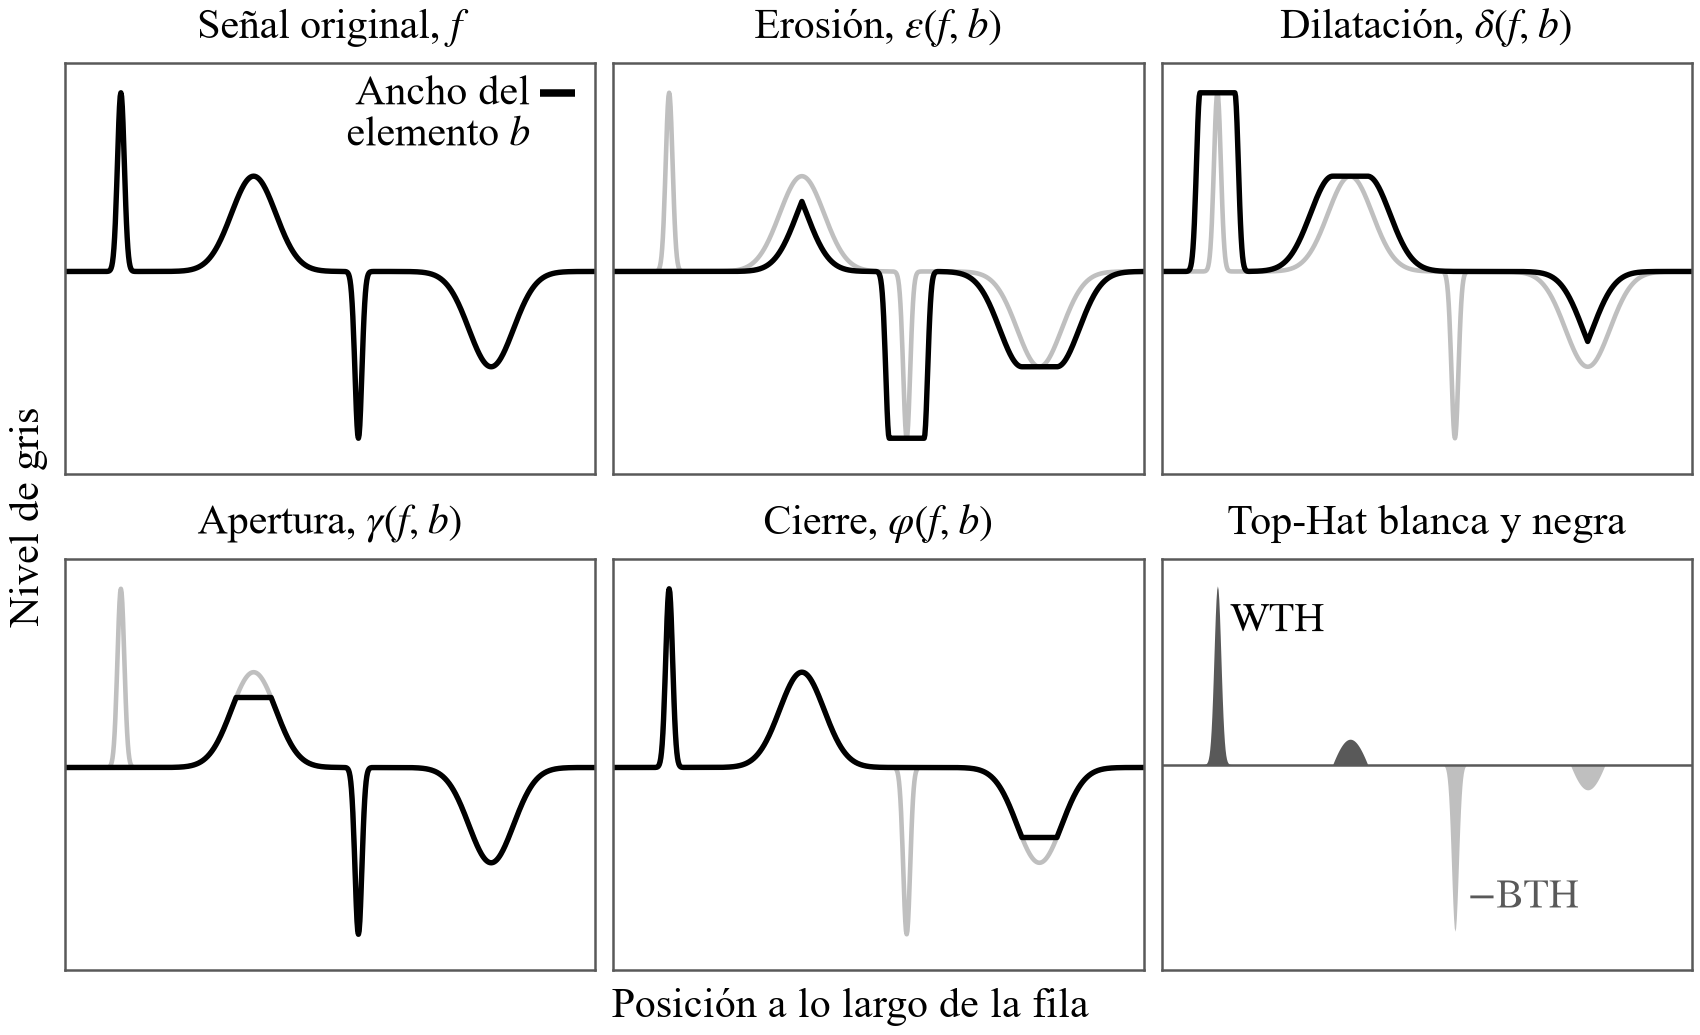
\includegraphics[width=0.9\textwidth]{figuras/fig_morfologia_tophat}
\nota{Elaboración propia. La barra del primer panel marca el ancho del elemento estructurante $b$. En
los cuatro paneles siguientes se repite en gris la señal original $f$. En el último, la Top-Hat blanca
se dibuja hacia arriba y la negra, con el signo cambiado, hacia abajo. Los montes y valles más
estrechos que $b$ pasan enteros a la Top-Hat; de los más anchos, solo pasa la parte más estrecha que $b$.}
\end{figure}

\subsection{Transformada Top-Hat}

La transformada Top-Hat mide cuánto cambia la imagen al aplicarle la apertura o el cierre. La Top-Hat
blanca (WTH, del inglés \textit{White Top-Hat}) es la imagen menos su apertura. La negra (BTH, del inglés
\textit{Black Top-Hat}) es el cierre menos la imagen \parencite{soille2003, gonzalez2018}:
\begin{equation} \mathrm{WTH}(f,b) = f - \gamma(f,b), \qquad \mathrm{BTH}(f,b) = \varphi(f,b) - f. \label{eq:wth-bth} \end{equation}
La blanca conserva los detalles claros más estrechos que el elemento, y la negra, los oscuros. Las dos
son mayores o iguales que cero, y casi nulas en las zonas planas o de variación suave. Así separan el
detalle fino, que queda en las dos Top-Hat, del fondo, que queda en la apertura y en el cierre.

\subsection{Tamaño y forma del elemento estructurante}

El tamaño del elemento fija la frontera entre el detalle y el fondo \parencite{soille2003, gonzalez2018}.
De cada monte o valle, la Top-Hat recoge la parte más estrecha que el elemento, y el resto queda en el
fondo. Con un elemento pequeño, la Top-Hat recoge solo la textura fina, las líneas delgadas y el ruido.
Con uno grande puede recoger además objetos enteros, como una persona o un vehículo que se destacan de su
entorno. En este trabajo el tamaño se expresa con un radio $r$, en píxeles, y cada elemento se extiende
unos $r$ píxeles a cada lado de su centro.

La forma del elemento decide en qué direcciones se mide ese ancho \parencite{serra1982, soille2003}. Un
disco mide lo mismo en todas las direcciones y no distingue la orientación de los detalles. Un segmento
de recta, en cambio, mira en una sola dirección. La apertura con un segmento conserva las estructuras
claras que se extienden en esa dirección al menos tanto como el segmento, y rebaja las demás. Por eso el
segmento no extrae las estructuras alineadas con él: como cabe en ellas, estas sobreviven a la apertura y
la Top-Hat vale cero allí. Extrae, en cambio, los detalles más angostos que su largo en esa dirección.
Así, un objeto alargado queda en el fondo con un segmento paralelo y pasa a la Top-Hat con uno
perpendicular más largo que su ancho.

\subsection{Realce de contraste}

La Top-Hat sirve también para realzar el contraste, es decir, para que un detalle se distinga mejor de
su entorno. Su forma más simple suma a la imagen su Top-Hat blanca y le resta la negra
\parencite{bai2012}:
\begin{equation} f_{\mathrm{R}} = f + \mathrm{WTH}(f,b) - \mathrm{BTH}(f,b). \label{eq:realce} \end{equation}
Aquí $f_{\mathrm{R}}$ es la imagen realzada. Los detalles claros se aclaran, los oscuros se oscurecen y
el fondo casi no cambia. Los trabajos de \textcite{mukhopadhyay2000} y \textcite{bai2012} llevan esta
idea a varias escalas, con elementos de tamaños crecientes. Algunos métodos morfológicos de fusión la
aplican a dos imágenes a la vez \parencite{bai2013, roman2020}, y así lo hace también el algoritmo
propuesto.

\subsection{Fusión basada en la transformada Top-Hat}
\label{sec:fusion-tophat}

En su versión más simple, la fusión basada en la transformada Top-Hat separa en cada fuente el detalle
del fondo y agrega el detalle de ambas a una imagen base común \parencite{roman2020,
ortegarodriguez2025}. La regla siguiente es común al Top-Hat clásico y a la propuesta. Retoma la de
\textcite{ortegarodriguez2025}, incluido el peso que regula cuánto detalle se agrega, y recorta el
resultado de forma explícita al intervalo de cero a uno. Sean $\mathrm{WTH}_{\mathrm{VIS}}$ y
$\mathrm{BTH}_{\mathrm{VIS}}$ las transformadas Top-Hat blanca y negra de la visible, y
$\mathrm{WTH}_{\mathrm{IR}}$ y $\mathrm{BTH}_{\mathrm{IR}}$ las de la infrarroja. La imagen fusionada es
\begin{equation} \begin{aligned} F = \operatorname{recorte}\Bigl( & \tfrac{1}{2}\bigl(I_{\mathrm{VIS}} + I_{\mathrm{IR}}\bigr)
 + m \max\bigl(\mathrm{WTH}_{\mathrm{VIS}},\, \mathrm{WTH}_{\mathrm{IR}}\bigr) \\
 & - m \max\bigl(\mathrm{BTH}_{\mathrm{VIS}},\, \mathrm{BTH}_{\mathrm{IR}}\bigr) \Bigr). \end{aligned} \label{eq:regla-tophat} \end{equation}
Aquí $m$ es un peso no negativo, y el máximo se toma píxel a píxel. La función
$\operatorname{recorte}(z) = \min\{1, \max\{0, z\}\}$ lleva a cero los valores negativos y a uno los
mayores que uno.

La regla parte del promedio de las dos fuentes, que hace de imagen base. En cada píxel toma el mayor
detalle claro y el mayor detalle oscuro de las dos fuentes, así que un detalle se conserva si al menos
una de las cámaras lo capta. El claro se suma a la base y el oscuro se resta. Como las transformadas
Top-Hat nunca son negativas, la suma aclara los detalles claros y la resta oscurece los oscuros. Así crece
el contraste local, la diferencia de brillo entre un detalle y su entorno. Con $m = 0$ la fusión es el
promedio simple, y cuanto mayor es $m$, más detalle se agrega. Un peso alto puede sacar más píxeles del
intervalo de cero a uno, que el recorte deja en negro o en blanco. El Top-Hat clásico sigue la fusión
con Top-Hat de \textcite{bajacfigueredo2024} y aplica esta regla con un único disco como elemento
estructurante.

\section{Métricas de evaluación sin referencia}
\label{sec:metricas}

La calidad de una fusión visible-infrarroja se estima con métricas que no necesitan una imagen fusionada
ideal \parencite{ma2019, singh2023}. Para \textcite{singh2023}, sin referencia son solo las que usan la
fusión sola; las que la comparan con las fuentes son de referencia parcial. Aquí se usan seis, en
dos grupos de tres. Las del primer grupo miden la actividad: cuánta información, cuánto contraste y
cuánta nitidez de bordes tiene la fusión por sí misma. Las del segundo miden la fidelidad, es decir,
cuánto se parece la fusión a cada fuente. En las seis, un valor mayor se considera mejor. En lo que
sigue, $F$ es la imagen fusionada, de $H$ filas y $W$ columnas, y $X$ designa una fuente, sea
$I_{\mathrm{VIS}}$ o $I_{\mathrm{IR}}$.

\subsection{Métricas de actividad}

Las tres métricas de actividad son la entropía (EN, del inglés \textit{Entropy}), la desviación estándar
(SD, del inglés \textit{Standard Deviation}) y el gradiente medio (MG, del inglés \textit{Mean Gradient}).

La entropía mide cuán repartidos están los píxeles entre los niveles de gris
\parencite{singh2023, ortegarodriguez2025}. Para calcularla, el
intervalo de cero a uno se divide en 256 tramos iguales, y $p_a$ es la proporción de píxeles de $F$ que
caen en el tramo $a$. Ese reparto se llama histograma. La entropía es
\begin{equation} \mathrm{EN}(F) = -\sum_{a=0}^{255} p_a \log_2 p_a. \label{eq:met-en} \end{equation}
Los tramos vacíos no aportan. Se mide en bits, la unidad de información, y alcanza su máximo, 8~bits,
cuando todos los tramos tienen la misma proporción.

La desviación estándar mide el contraste general, es decir, cuánto se alejan en promedio las
intensidades de su valor medio $\mu_F$ \parencite{singh2023, ortegarodriguez2025}. Una imagen de tono
parejo tiene una desviación baja, y una con zonas muy claras junto a zonas muy oscuras la tiene alta. Se
calcula como
\begin{equation} \mathrm{SD}(F) = \sqrt{\frac{1}{HW}\sum_{x=1}^{W}\sum_{y=1}^{H}\bigl(F(x,y)-\mu_F\bigr)^2}, \qquad \mu_F = \frac{1}{HW}\sum_{x=1}^{W}\sum_{y=1}^{H}F(x,y). \label{eq:met-sd} \end{equation}
Aquí $F(x,y)$ es la intensidad del píxel de la columna $x$ y la fila $y$. La suma de cuadrados se
divide por el número total de píxeles, $HW$. Como las intensidades van de cero a uno, SD no puede
superar 0.5. Su cuadrado se llama varianza.

El gradiente medio mide la nitidez de los bordes \parencite{singh2023}. El gradiente indica cuánto cambia
la intensidad de un píxel a sus vecinos, y crece donde la imagen salta de claro a oscuro. En el interior
de la imagen se calcula con diferencias centrales, entre el vecino anterior y el siguiente:
\begin{equation} G_x(x,y) = \frac{F(x+1,y)-F(x-1,y)}{2}, \qquad G_y(x,y) = \frac{F(x,y+1)-F(x,y-1)}{2}. \label{eq:met-gradiente} \end{equation}
Aquí $G_x$ es el cambio horizontal y $G_y$ el vertical. En las filas y columnas extremas, donde falta un
vecino, se usa la diferencia con el único disponible, sin dividir por dos. Así,
\begin{equation} \mathrm{MG}(F) = \frac{1}{HW}\sum_{x=1}^{W}\sum_{y=1}^{H}\sqrt{G_x(x,y)^2+G_y(x,y)^2}. \label{eq:met-mg} \end{equation}
El valor depende de la fórmula de las diferencias, así que solo se comparan valores calculados de la
misma manera.

\subsection{Métricas de fidelidad}

Las tres métricas de fidelidad son la información mutua (MI, del inglés \textit{Mutual Information}), la
similitud estructural (SSIM, del inglés \textit{Structural Similarity}) y la relación señal-ruido de pico
(PSNR, del inglés \textit{Peak Signal-to-Noise Ratio}).

La información mutua mide cuánto baja la incertidumbre sobre el nivel de gris de un píxel en una fuente
$X$ al conocer su nivel en $F$ \parencite{qu2002}. Para calcularla, cada intensidad se multiplica por 63
y se trunca al entero inferior, lo que deja 64 niveles. Con ellos se arma el histograma conjunto, donde
$p_{FX}(a,c)$ es la proporción de píxeles con nivel $a$ en $F$ y nivel $c$ en $X$. Así,
\begin{equation} \mathrm{MI}(F,X) = \sum_{a=0}^{63}\sum_{c=0}^{63} p_{FX}(a,c)\,\log_2\frac{p_{FX}(a,c)}{p_F(a)\,p_X(c)}. \label{eq:met-mi} \end{equation}
Aquí $p_F(a)$ y $p_X(c)$ son las proporciones en cada imagen sola, y las casillas vacías no aportan. La
métrica del trabajo promedia las dos fuentes en cada par de imágenes:
\begin{equation} \mathrm{MI} = \tfrac{1}{2}\bigl[\mathrm{MI}(F,I_{\mathrm{VIS}})+\mathrm{MI}(F,I_{\mathrm{IR}})\bigr]. \label{eq:met-mi-promedio} \end{equation}
Si se sumaran los dos términos, el valor se duplicaría sin cambiar el orden de los métodos.

El índice de similitud estructural compara dos imágenes por zonas pequeñas, o ventanas
\parencite{wang2004}. En cada ventana $w$ compara el brillo medio, el contraste y el patrón de variación
de $X$ y de $F$:
\begin{equation} \mathrm{SSIM}_w(X,F) = \frac{(2\mu_X\mu_F + C_1)(2\sigma_{XF} + C_2)}{(\mu_X^2+\mu_F^2+C_1)(\sigma_X^2+\sigma_F^2+C_2)}. \label{eq:met-ssim} \end{equation}
Aquí $\mu_X$ y $\mu_F$ son las medias en la ventana, $\sigma_X^2$ y $\sigma_F^2$ las varianzas, y
$\sigma_{XF}$ la covarianza, que mide cuánto varían juntas. Las constantes $C_1=(0.01)^2$ y
$C_2=(0.03)^2$ evitan dividir por cero. En este trabajo la ventana mide $7 \times 7$ píxeles, todos
con el mismo peso, y las varianzas y la covarianza se dividen por 48. La versión original usa una ventana mayor que
pesa más el centro \parencite{wang2004}. El índice promedia $\mathrm{SSIM}_w$ sobre las ventanas que
caben enteras, y la métrica final promedia las dos fuentes:
\begin{equation} \mathrm{SSIM} = \tfrac{1}{2}\bigl[\mathrm{SSIM}(I_{\mathrm{VIS}},F)+\mathrm{SSIM}(I_{\mathrm{IR}},F)\bigr]. \label{eq:met-ssim-promedio} \end{equation}

La relación señal-ruido de pico expresa el error numérico entre dos imágenes en escala logarítmica, que
reúne en un rango corto valores muy distintos \parencite{singh2023}. Se apoya en el error cuadrático
medio (MSE, del inglés \textit{Mean Squared Error}), el promedio de los cuadrados de las diferencias
píxel a píxel. Siguiendo a \textcite{ortegarodriguez2025}, primero se promedian los errores frente a
las dos fuentes y después se toma el logaritmo. Así,
\begin{equation} \begin{aligned} \mathrm{MSE}(F,X) &= \frac{1}{HW}\sum_{x=1}^{W}\sum_{y=1}^{H}\bigl(F(x,y)-X(x,y)\bigr)^2,\\
 \mathrm{PSNR} &= 10\log_{10}\frac{1}{\tfrac{1}{2}\bigl[\mathrm{MSE}(F,I_{\mathrm{VIS}})+\mathrm{MSE}(F,I_{\mathrm{IR}})\bigr]}. \end{aligned} \label{eq:met-psnr} \end{equation}
El 1 del numerador es el cuadrado de la mayor intensidad posible. La PSNR se mide en decibelios, la
unidad de esa escala, y un valor alto indica que la fusión se aparta poco de sus fuentes. En la escala de
0 a 255 el valor no cambia, porque el numerador y el error crecen en la misma proporción. Promediar los
errores no equivale a promediar las dos PSNR.

\subsection{Selección de las seis métricas}

Las seis resultan de depurar con dos criterios una batería inicial de nueve métricas. Esa batería
incluye las cinco que usan \textcite{ortegarodriguez2025}. El primer criterio es no repetir información. La
eficiencia de fusión (FE, del inglés \textit{Fusion Efficiency}) divide la EN de la fusión por la EN
media de las fuentes. Como ese divisor es fijo en cada par, FE ordena los métodos igual que EN. La
frecuencia espacial (SF, del inglés \textit{Spatial Frequency}) mide el cambio entre píxeles vecinos
\parencite{eskicioglu1995}, casi lo mismo que MG. La batería contaba aparte la MI con cada fuente, lo
que duplicaba su peso. Sin esas tres repeticiones quedan las seis. El segundo criterio es el equilibrio.
La actividad sube también con el ruido, y la fidelidad, con solo copiar las fuentes; por eso los dos
grupos tienen tres métricas cada uno.

\subsection{Métricas complementarias}

Otras ocho métricas se calculan solo como comprobación, y el Capítulo~\ref{cap:resultados} las usa con
ese fin. El índice de información de bordes (Qabf) mide cuánta información de bordes pasa de las fuentes
a la fusión \parencite{xydeas2000}. La medida de ruido y artefactos de fusión (Nabf) se propuso después en
ese marco \parencite{petrovic2005}. Pondera los píxeles donde la fusión tiene bordes más fuertes que las
dos fuentes, y es la única en que un valor menor es mejor. Aquí se usa la ponderación modificada de
\textcite{kumar2013}. La suma de las correlaciones de las diferencias (SCD, del inglés \textit{Sum of the
Correlations of Differences}) suma, para cada fuente, su correlación con la diferencia entre la imagen
fusionada y la otra fuente \parencite{aslantas2015}. La fidelidad de la información visual (VIF, del
inglés \textit{Visual Information Fidelity}) mide cuánta información visual de un original conserva otra
imagen \parencite{sheikh2006}; aquí, el original es cada fuente. La información mutua de
características (FMI, del inglés \textit{Feature Mutual Information}) aplica la información mutua a los
gradientes \parencite{haghighat2011}. Las tres variantes de \textcite{piella2003} calculan por
ventanas el índice de la Ecuación~\eqref{eq:met-ssim} sin $C_1$ ni $C_2$ y combinan esos valores con
distintos pesos. Son el índice ponderado por la varianza local (Q0), el ponderado por ventana (QW) y el
de bordes (QE). En el primero, el índice de cada fuente pesa en cada ventana según su varianza local. El
segundo da además más peso a las ventanas de mayor varianza, y el tercero multiplica QW por el mismo
índice calculado sobre los bordes de las imágenes. En esa obra el primero se llama Q; aquí figura como
Q0, aunque sus autores reservan ese nombre para el índice sin ponderar. Las ocho comparan la fusión con
sus fuentes, y sumarlas inclinaría el equilibrio hacia la fidelidad.

\section{Pruebas estadísticas}
\label{sec:pruebas}

Para comparar la calidad de los métodos se usan pruebas no paramétricas, que no suponen una distribución
normal de los datos. La prueba de Friedman \parencite{friedman1937} trata cada par de imágenes como un bloque:
ordena los métodos dentro de cada par y pregunta si alguno tiende a quedar mejor o peor ubicado. La prueba de
Wilcoxon de rangos con signo \parencite{wilcoxon1945} compara dos métodos a partir de sus diferencias en
los mismos pares. Cada prueba da un valor de $p$: la probabilidad de ver una diferencia al menos tan
grande si los métodos fueran iguales. Como las comparaciones por pares son muchas, esos valores se
corrigen con el procedimiento de \textcite{holm1979}. Ese procedimiento los ordena de menor a mayor y los
compara con umbrales que empiezan muy estrictos y se aflojan paso a paso.

Cuando las observaciones de un mismo grupo no son independientes, como los cuadros de un mismo tramo de
video, el error estándar se calcula por grupos y no por observación \parencite{cameron2015}. Con pocos
grupos, ese error tiende a subestimar la variación, y el \textit{bootstrap} salvaje por grupos
estudentizado ofrece una prueba más confiable \parencite{cameron2008, webb2023}. Este repite el cálculo
miles de veces, con el aporte de cada grupo multiplicado por un peso al azar, y en cada repetición
divide la estimación por su propio error estándar. La correlación de rangos de Spearman
\parencite{spearman1904}, por último, mide cuánto coinciden dos ordenamientos de los mismos elementos.

\section{Optimización por enjambre de partículas}
\label{sec:pso}

La optimización por enjambre de partículas (PSO, del inglés \textit{Particle Swarm Optimization}) es un
método de búsqueda propuesto por \textcite{kennedy1995}. El método mueve un grupo de soluciones
posibles, llamadas partículas, dentro de una región de búsqueda. En la fusión de imágenes, \textcite{tao2010}
combinan la PSO con la DTCWT, y \textcite{malviya2014}, con la transformada \textit{wavelet}. Por su parte,
\textcite{ortegarodriguez2025} la aplican a los parámetros de la transformada Top-Hat en la fusión
visible-infrarroja.

La búsqueda avanza por iteraciones, es decir, por pasos sucesivos. En la iteración $t$, la partícula
$i$ ocupa la posición $\mathbf{x}_i^{t}$ y tiene la velocidad $\mathbf{v}_i^{t}$, que indica hacia
dónde y cuánto se desplaza. Al comenzar, las posiciones y las
velocidades se sortean al azar. Cada partícula recuerda la mejor posición que ha visitado,
$\mathbf{p}_i^{t}$, y conoce la mejor posición del grupo, $\mathbf{g}^{t}$. Para decidir cuál es mejor
se usa una función de aptitud, que asigna a cada posición un número, mayor cuanto mejor es la solución.
En cada iteración se evalúan las partículas y se actualizan esas mejores posiciones. Luego cada partícula
cambia su velocidad:
\begin{equation} \mathbf{v}_i^{t+1} = w_t\,\mathbf{v}_i^{t} + c_1\,\boldsymbol{\rho}_1 \odot \bigl(\mathbf{p}_i^{t} - \mathbf{x}_i^{t}\bigr) + c_2\,\boldsymbol{\rho}_2 \odot \bigl(\mathbf{g}^{t} - \mathbf{x}_i^{t}\bigr). \label{eq:pso-velocidad} \end{equation}
Con ella, la nueva posición es
\begin{equation} \mathbf{x}_i^{t+1} = \min\bigl(\max\bigl(\mathbf{x}_i^{t} + \mathbf{v}_i^{t+1},\, \mathbf{x}_{\min}\bigr),\, \mathbf{x}_{\max}\bigr). \label{eq:pso-posicion} \end{equation}

Los vectores $\boldsymbol{\rho}_1$ y $\boldsymbol{\rho}_2$ contienen números al azar entre cero y uno,
todos igual de probables. Se sortean de nuevo en cada iteración, para cada partícula y cada coordenada.
El símbolo $\odot$ indica el producto coordenada a coordenada. Los coeficientes $c_1$ y $c_2$ regulan
la atracción hacia la mejor posición propia y hacia la del grupo. En la
Ecuación~\eqref{eq:pso-posicion}, el mínimo y el máximo mantienen cada coordenada dentro de los límites
$\mathbf{x}_{\min}$ y $\mathbf{x}_{\max}$ de la región de búsqueda. El factor $w_t$, llamado inercia,
regula cuánto conserva cada partícula de su velocidad anterior. Ese factor no figura en la versión
original de \textcite{kennedy1995}; lo introducen \textcite{shi1998}.

Cuando la inercia decrece en línea recta a lo largo de las $T$ iteraciones, va de $w_{\max}$ en la
primera a $w_{\min}$ en la última. Su valor en la iteración $t$ es entonces
\begin{equation} w_t = w_{\max} - \left(w_{\max} - w_{\min}\right)\frac{t}{T-1}, \qquad t = 0, 1, \ldots, T-1. \label{eq:pso-inercia} \end{equation}
Con una inercia alta pesa más la velocidad anterior, y con una baja, la atracción hacia las mejores
posiciones halladas. Al terminar las iteraciones, la solución es la mejor posición del grupo.

\section{Detección de objetos}
\label{sec:marco-deteccion}

\subsection{Funcionamiento de un detector}

La detección automática de objetos consiste en encontrar y ubicar en una imagen los objetos de ciertas
clases, como personas o luces. El detector se entrena con imágenes en las que cada objeto está marcado
con una caja rectangular y su clase. Luego, ante una imagen nueva, devuelve predicciones: cajas con una
clase y un puntaje de confianza, que indica cuán seguro está el modelo. El detector YOLO
(del inglés \textit{You Only Look Once}, \enquote{solo se mira una vez}) propone las cajas y sus clases
en una sola pasada, al ritmo del video \parencite{redmon2016}. Su octava versión, YOLOv8, es de libre
distribución y ofrece cinco tamaños y pesos preentrenados, es decir, valores internos ya aprendidos con
otras imágenes \parencite{jocher2023}.

\subsection{Intersección sobre la unión, precisión y exhaustividad}

Para juzgar una predicción, su caja $B$ se compara con la caja marcada $A$. Se usa la intersección sobre
la unión (IoU, del inglés \textit{Intersection over Union}), con la que YOLO define también la
confianza de sus cajas \parencite{redmon2016}:
\begin{equation} \mathrm{IoU}(A,B)=\frac{\lvert A\cap B\rvert}{\lvert A\rvert+\lvert B\rvert-\lvert A\cap B\rvert}. \label{eq:iou} \end{equation}
Aquí $A\cap B$ es la zona común a las dos cajas, y $\lvert\cdot\rvert$ indica el área. La IoU vale uno si
las cajas coinciden y cero si no se superponen. Solo cuentan las predicciones cuyo puntaje de confianza
alcanza un umbral. Cada objeto marcado se une, como máximo, a una predicción de su misma clase: la de
mayor IoU entre las que siguen libres. En este trabajo, si esa IoU alcanza 0.5, el objeto cuenta como
encontrado. Ese umbral es el del desafío de reconocimiento visual de objetos PASCAL VOC (del inglés
\textit{Pattern Analysis, Statistical Modelling and Computational Learning Visual Object Classes}),
descrito por \textcite{everingham2010}. La predicción es entonces un verdadero positivo, $\mathit{VP}$,
y deja de estar libre.

Las predicciones que quedan libres son falsos positivos, $\mathit{FP}$, y los objetos sin pareja, falsos
negativos, $\mathit{FN}$. Con esos conteos se definen la precisión $P$ y la exhaustividad $R$:
\begin{equation} P=\frac{\mathit{VP}}{\mathit{VP}+\mathit{FP}},\qquad R=\frac{\mathit{VP}}{\mathit{VP}+\mathit{FN}}. \label{eq:precision-exhaustividad} \end{equation}
La primera mide qué parte de las predicciones es correcta; la segunda, qué parte de los objetos se
encuentra. Ambas dependen del umbral de confianza. Al bajarlo, $R$ crece o se mantiene, y $P$ suele
caer. La exhaustividad se llama también tasa de acierto. Calculada sobre un grupo elegido de objetos, es
la base de la medida de detección de este trabajo, descrita en la Sección~\ref{sec:protocolo-deteccion}.

\subsection{Precisión media}

La precisión media (AP, del inglés \textit{Average Precision}) resume la relación entre $P$ y $R$ en
todos los umbrales de confianza. Se calcula para cada clase por separado:
\begin{equation} \mathrm{AP}=\int_{0}^{1}\tilde{P}(R)\,dR. \label{eq:ap} \end{equation}
Aquí $\tilde{P}(R)$ es la mayor precisión lograda con una exhaustividad de $R$ o más. La integral se
aproxima con 101 valores de $R$ repartidos por igual entre cero y uno, como hace la biblioteca
Ultralytics \parencite{jocher2023}. La AP depende también del umbral
de IoU que decide los aciertos; con 0.5 se escribe AP50. La mAP50 es la media de la AP50 sobre las $C$
clases con objetos marcados:
\begin{equation} \mathrm{mAP50}=\frac{1}{C}\sum_{c=1}^{C}\mathrm{AP50}_c. \label{eq:map50} \end{equation}
Aquí $\mathrm{AP50}_c$ es la de la clase $c$.

\subsection{La detección como evaluación de la fusión}

La detección sirve también para evaluar una fusión. Esa evaluación exige cuidado, porque un detector
aprende la apariencia de sus imágenes de entrenamiento, como el contraste y la textura. Si se lo aplica
sin reentrenar a imágenes de otro aspecto, su acierto puede caer, como muestran \textcite{redmon2016}
con pinturas. Así, el resultado de la detección puede reflejar en parte ese cambio de aspecto, y no solo la utilidad
de la fusión.
Para comparar métodos en igualdad de condiciones, \textcite{liu2022} entrenan un detector con las
imágenes fusionadas de cada uno. Este trabajo sigue esa práctica, como detalla la
Sección~\ref{sec:protocolo-deteccion}.

\section{Estado del arte y brecha existente}
\label{sec:estado-arte}

Entre los antecedentes de fusión basados en la transformada Top-Hat, \textcite{bai2011} extraen de las
fuentes sus regiones claras y oscuras de varias escalas con una Top-Hat de centro y entorno
(\textit{center-surround}). Esas regiones se incorporan a una imagen base calculada a partir de las
fuentes. Más adelante, \textcite{bai2013} propone una fusión morfológica que extrae las regiones con una
Top-Hat multiescala, es decir, repetida con elementos de tamaño creciente. Los detalles los extrae con un
operador de contraste por conmutación (\textit{toggle contrast operator}). A su vez, \textcite{zhu2017}
mejoran la Top-Hat de centro y entorno de varias escalas, y proponen una regla para fusionar las regiones
de cada escala y otra para formar la imagen base. Dos años después, \textcite{saravia2019} extraen
las regiones claras y oscuras con una Top-Hat multiescala y dos elementos estructurantes. En la
Universidad Nacional de Asunción, \textcite{roman2020} proponen otro método morfológico multiescala
para fusionar imágenes visibles e infrarrojas. Ese trabajo y el de \textcite{saravia2019} se publicaron
en el marco de la tesis doctoral de \textcite{melloroman2021}, que reúne esquemas Top-Hat multiescala
para la mejora y la fusión de imágenes. Todos ellos operan en varias escalas; el algoritmo
propuesto, en una sola. La Top-Hat se aplica también a otros pares de imágenes. Con una visible en color
y una infrarroja cercana, no térmica, \textcite{herreraarellano2021} fusionan de forma selectiva las
estructuras más relevantes para mejorar fotografías de exteriores degradadas por el mal tiempo.

El antecedente directo es el trabajo de \textcite{bajacfigueredo2024}, entre cuyos autores figuran los
de esta tesis. Ese trabajo aplica la Top-Hat a la fusión de imágenes infrarrojas y visibles. Después,
\textcite{ortegarodriguez2025} emplean una regla con un peso que regula cuánto detalle se agrega, y
ajustan ese peso y el radio del disco con optimización por enjambre de partículas.

El banco de cinco elementos estructurantes del algoritmo propuesto, un disco y cuatro segmentos
orientados, se diseñó para el realce de mamografías \parencite{floressf}. Ese trabajo lo usa con una
Top-Hat de varias escalas. La forma de combinar sus respuestas proviene del realce de imágenes de fondo
de ojo \parencite{bala2024}. Ninguno de los trabajos revisados aplica ese banco a la fusión
visible-infrarroja.

Las métricas sin referencia juzgan la imagen o su parecido con las fuentes, pero no su utilidad para una
tarea. Una alternativa reciente evalúa la fusión por su efecto en una tarea de alto nivel, es decir, una
que interpreta la escena, como detectar objetos. En esa línea, \textcite{liu2022} orientan su red de
fusión a los objetos de interés y publican M3FD, un conjunto de pares con objetos marcados. Por su parte,
\textcite{tang2022} entrenan la red de fusión junto con una de segmentación, que asigna cada píxel a una
clase de objeto. Esos trabajos presentan redes neuronales de fusión guiadas por la tarea. Para el banco
de cinco elementos, la literatura revisada no ofrece una evaluación de ese tipo.

Esos dos vacíos, el uso del banco en la fusión visible-infrarroja y su evaluación por una tarea, forman
la brecha que aborda este trabajo. A diferencia de las redes guiadas por la tarea, el algoritmo
propuesto no aprende de la detección: la tarea solo sirve para evaluarlo.

\chapter{Metodología}
\label{cap:metodologia}

Este capítulo expone cómo se construyó el algoritmo propuesto y cómo se lo evaluó. Después del enfoque
y las variables del estudio, la Sección~\ref{sec:corpus} presenta los conjuntos de imágenes. La
Sección~\ref{sec:propuesta} define el algoritmo y los métodos comparativos, y la
Sección~\ref{sec:ajuste} describe el ajuste de su radio y su peso. Siguen la evaluación de la calidad
(Sección~\ref{sec:protocolo-calidad}), la de la aplicación a la detección
(Sección~\ref{sec:protocolo-deteccion}) y el examen de la hipótesis
(Sección~\ref{sec:examen-hipotesis}). La Figura~\ref{fig:metodologia} reúne esas etapas en un diagrama.
En él, los dos conjuntos de imágenes reciben el mismo preprocesamiento y se fusionan con los mismos siete
métodos. A partir de ahí el diagrama se abre: la rama izquierda lleva a la evaluación de la calidad, con
el conjunto TNO, y la derecha, a la de la detección, con el conjunto M3FD. Las dos ramas terminan en el
examen de la hipótesis. La flecha doble indica que el enjambre evalúa el propio algoritmo y le devuelve
el radio y el peso.

\begin{figure}[htbp]
\centering
\caption{Etapas del estudio}
\label{fig:metodologia}
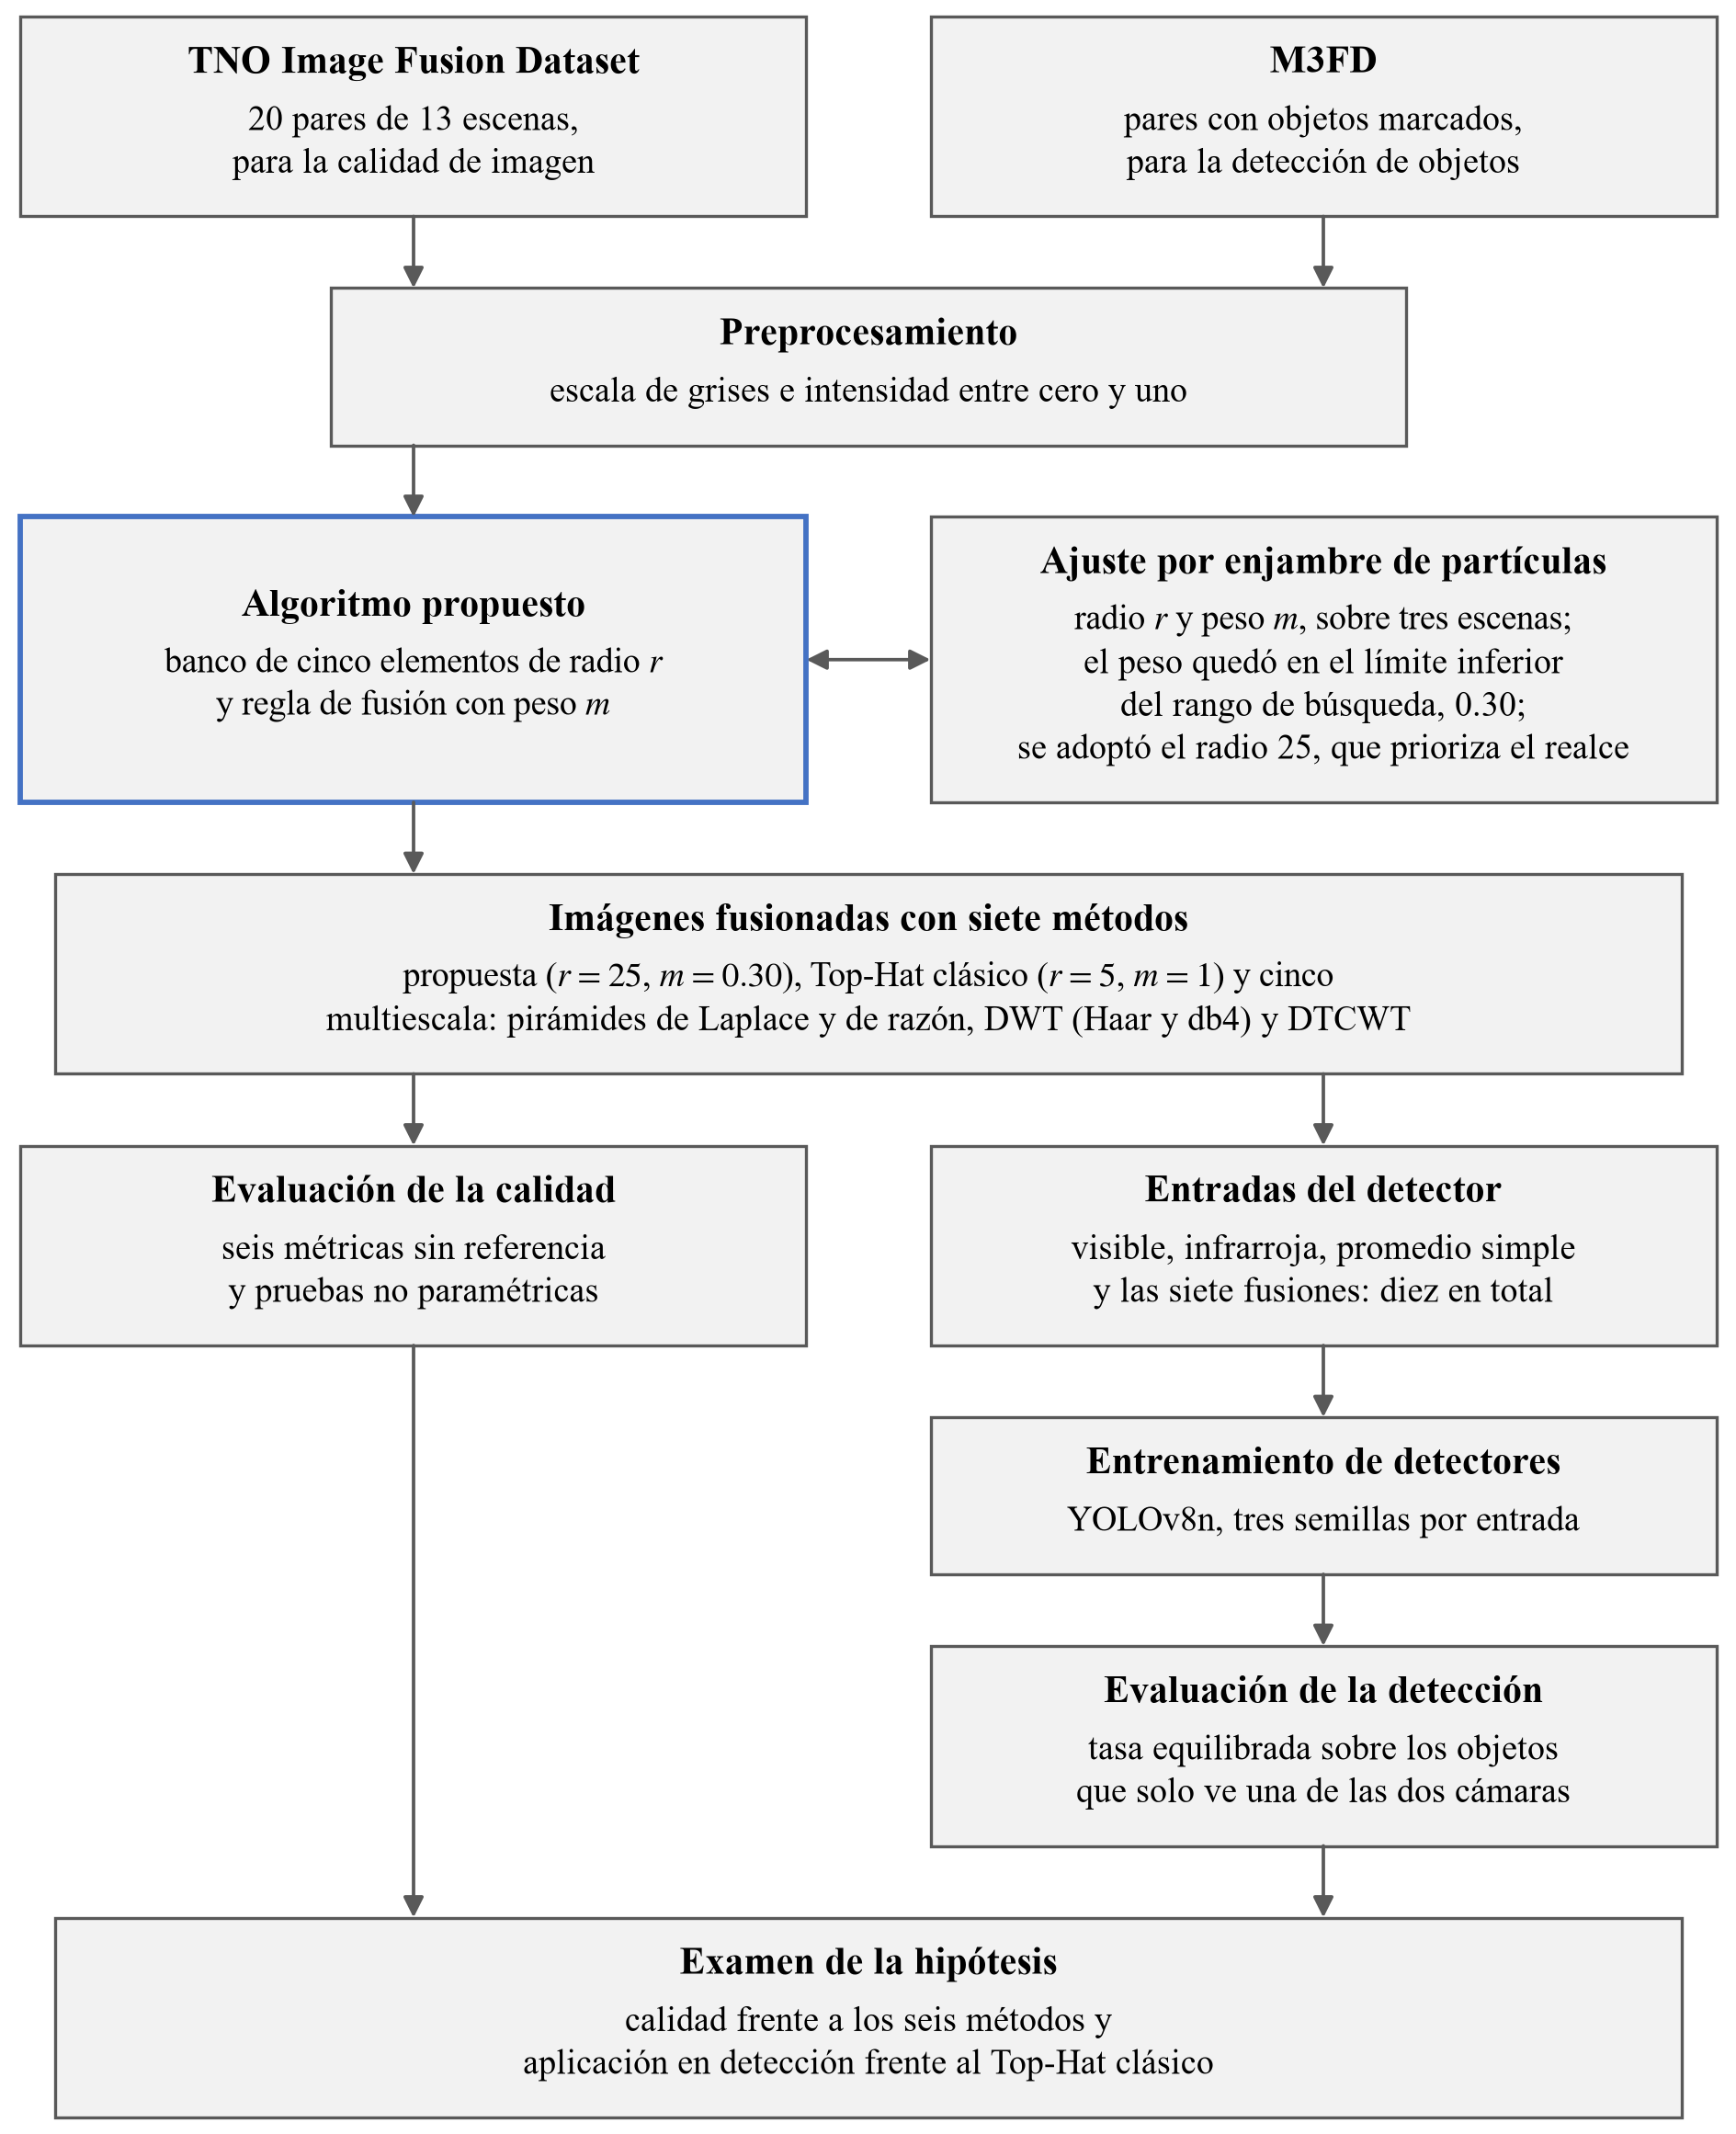
\includegraphics[width=\textwidth]{figuras/fig_metodologia}
\nota{Elaboración propia. El recuadro azul destaca el algoritmo propuesto.}
\end{figure}

El enfoque fue cuantitativo. Cada conclusión se apoyó en mediciones numéricas sobre conjuntos fijos de
imágenes, analizadas con pruebas estadísticas o, donde no hubo una prueba propia, de forma descriptiva, y no en el juicio de observadores. El diseño fue
experimental y comparativo. Todos los métodos procesaron las mismas imágenes y se midieron con el mismo
procedimiento, de modo que de una condición a otra solo varió la forma de fusionar.

La evaluación se hizo en dos planos. El primero es la calidad de la imagen fusionada, juzgada por sí
misma con métricas numéricas. El segundo es su aplicación, es decir, cuánto le sirve esa imagen a un
detector automático de objetos. Cada plano usa su propio conjunto de imágenes y se informa por
separado, porque un método puede destacar en uno y no en el otro.

Las variables del estudio fueron las siguientes:
\begin{itemize}
\item \textbf{Variable independiente:} El método de fusión. En la evaluación de calidad tomó siete
valores: el algoritmo propuesto, el Top-Hat clásico y cinco métodos multiescala. En la detección hubo
diez entradas para el detector: la imagen visible, la infrarroja, el promedio simple de ambas y las
siete fusiones.
\item \textbf{Variables dependientes:} Las seis métricas de calidad de imagen y la tasa de acierto
equilibrada del detector sobre los objetos vistos por una sola cámara.
\item \textbf{Variables controladas:} En la calidad, los pares de imágenes, el preprocesamiento y el
cálculo de las métricas. En la detección, los cuadros, las etiquetas de los objetos y la configuración
del detector.
\end{itemize}

\section{Conjuntos de imágenes y preprocesamiento}
\label{sec:corpus}

La calidad de imagen se midió sobre el \textit{TNO Image Fusion Dataset} \parencite{toet2014, toet2017}. El
conjunto reúne pares de imágenes nocturnas de escenas militares y de vigilancia, captados a la vez por una cámara
visible y por una térmica. En buena parte de los pares, la visible proviene de una cámara con
intensificador de imagen, que amplifica la escasa luz nocturna. El TNO es el conjunto público más usado
en la fusión visible-infrarroja \parencite{liu2022}, lo que facilita situar los resultados junto a los de
otros trabajos.

Los pares vienen registrados por sus autores: las dos imágenes de cada par cubren la misma escena desde
el mismo punto de vista. Aun así, en algunos se advierte un corrimiento vertical de varios píxeles entre
ambas. Ese corrimiento no se corrigió, para trabajar con el conjunto tal como se distribuye, y tampoco
se midió su efecto.

Se trabajó con veinte pares, que corresponden a trece escenas. Cuatro de esas escenas aportan más de una
toma, en otro instante o desde otro ángulo, y entre ellas reúnen once pares. La distinción tiene peso en
la estadística, porque dos tomas de una misma escena no son observaciones del todo independientes. La
Sección~\ref{sec:protocolo-calidad} explica cómo se tuvo en cuenta esa dependencia. También se comprobó
que en ningún par la imagen visible fuera una copia de la infrarroja.

El preprocesamiento se limitó a lo indispensable. Cada imagen se convirtió a escala de grises y sus
niveles se llevaron al intervalo de cero a uno con la Ecuación~\eqref{eq:intensidad}. No se aplicó
ningún realce, filtrado ni corrección de contraste previos, porque su efecto se habría confundido con el
del método de fusión.

La aplicación a la detección se evaluó sobre M3FD \parencite{liu2022}, un conjunto de 4200 pares
visible-infrarrojo registrados. Cada objeto está marcado con una caja y pertenece a una de seis clases:
personas, autos, autobuses, motocicletas, luces y camiones. Las escenas, urbanas y naturales, se tomaron
de día y de noche. Este conjunto se usó solo para la detección. Se le aplicó el mismo preprocesamiento
que al TNO, y por eso el detector recibió la imagen visible en escala de grises. Las imágenes de todas las entradas del detector
se guardaron en formato JPEG (del inglés \textit{Joint Photographic Experts Group}) de 8 bits. La
Sección~\ref{sec:det-datos} describe cómo se repartieron sus cuadros.

\section{El algoritmo de fusión propuesto}
\label{sec:propuesta}

El algoritmo propuesto es un operador Top-Hat de una sola escala: todos sus elementos estructurantes
comparten un mismo tamaño. Para fusionar aplica la regla de la Ecuación~\eqref{eq:regla-tophat}, que
retoma la de \textcite{ortegarodriguez2025}. Esa regla parte del promedio de las dos fuentes, le suma el mayor
detalle claro y le resta el mayor detalle oscuro, ambos multiplicados por el peso $m$. Lo nuevo está en
la manera de extraer ese detalle. En lugar de un disco único se usa el banco de cinco elementos
estructurantes de \textcite{floressf}, que lo emplean para realzar mamografías con una Top-Hat de varias
escalas. Aquí se lo aplica en una sola escala, y sus respuestas se combinan como proponen
\textcite{bala2024} para el realce de imágenes de fondo de ojo.

\subsection{Banco de elementos estructurantes}

El banco consta de un disco y cuatro segmentos de recta, definidos todos por un mismo radio $r$, que es
un número entero de píxeles. El disco $D_r$ es la versión digital de un círculo de radio $r$:
\begin{equation} D_r = \Bigl\{ (j,k) \in \mathbb{Z}^2 : |k| \le r,\ |j| \le \bigl\lfloor \sqrt{r^2 - k^2} + \tfrac{1}{2} \bigr\rfloor \Bigr\}. \label{eq:disco} \end{equation}
Cada par de enteros $(j,k)$ indica la posición de un píxel respecto del centro, en columnas y en filas.
La expresión $\lfloor u + \tfrac{1}{2} \rfloor$ redondea el número $u$ al entero más cercano. Con esa
definición, el disco mide $2r+1$ píxeles de ancho y otros tantos de alto.

Los cuatro segmentos, $S_{r,\theta}$, cruzan el centro con orientaciones de $0^\circ$, $45^\circ$,
$90^\circ$ y $135^\circ$. Como es habitual en imágenes, las filas se numeran hacia abajo, y por eso el
segmento de $45^\circ$ desciende de izquierda a derecha. Los segmentos quedan definidos así:
\begin{equation} \begin{aligned} S_{r,0^\circ}&=\{(j,0):|j|\le r\}, &\qquad S_{r,90^\circ}&=\{(0,k):|k|\le r\},\\
 S_{r,45^\circ}&=\{(j,j):|j|\le q_r\}, &\qquad S_{r,135^\circ}&=\{(-j,j):|j|\le q_r\}. \end{aligned} \label{eq:segmentos} \end{equation}
Aquí, $q_r = \lfloor r/\sqrt{2} + \tfrac{1}{2} \rfloor$. El segmento horizontal y el vertical tienen
$2r+1$ píxeles, lo mismo que el ancho del disco. Los diagonales tienen $2q_r+1$, porque en diagonal la
distancia entre píxeles vecinos es mayor. Cubren así casi la misma longitud con menos píxeles. Con
$r = 25$, el disco y los segmentos horizontal y vertical miden 51 píxeles; los diagonales, 37.

La Figura~\ref{fig:banco_se} dibuja píxel por píxel los cinco elementos del banco, con un radio menor,
$r = 5$, para que los píxeles se distingan. Los cinco comparten el mismo centro. Con ese radio, el disco
coincide con el único elemento del Top-Hat clásico (Sección~\ref{sec:operador}).

\begin{figure}[htbp]
\centering
\caption{Banco de cinco elementos estructurantes del algoritmo propuesto}
\label{fig:banco_se}
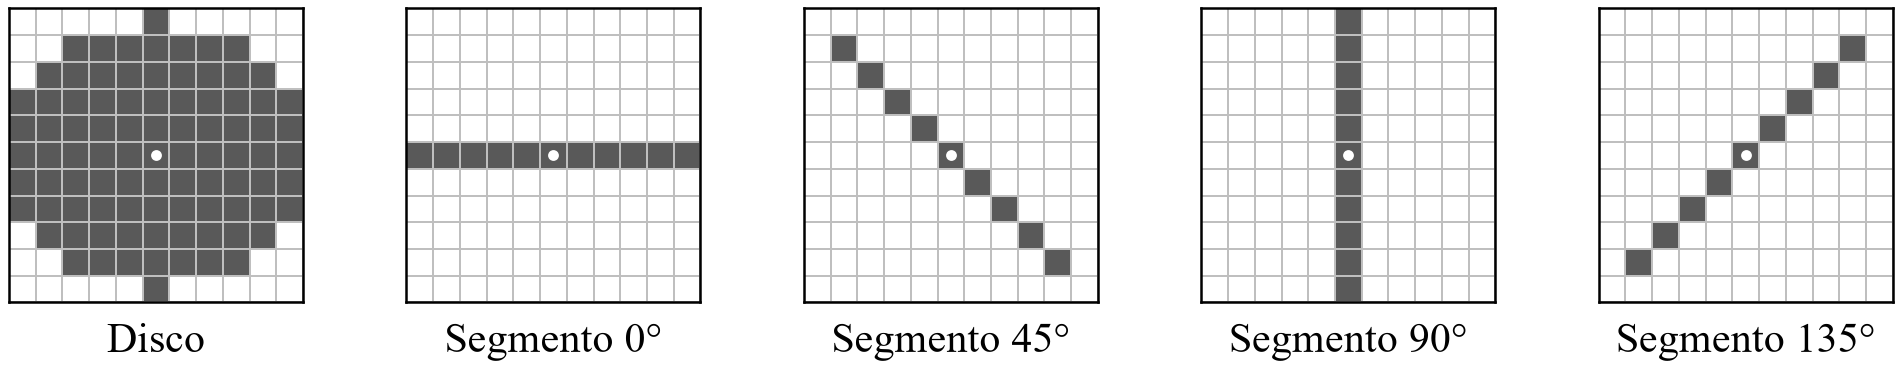
\includegraphics[width=\textwidth]{figuras/fig_banco_se}
\nota{Elaboración propia. Cada cuadro es un píxel; los cuadros grises forman el elemento, y el punto
blanco marca su centro. Con $r = 5$, cada cuadrícula mide $11 \times 11$ píxeles, y los segmentos
diagonales tienen 9 píxeles en lugar de 11. Con la configuración adoptada, $r = 25$, cada elemento ocupa
una cuadrícula de $51 \times 51$ píxeles. El disco termina en un solo píxel arriba y abajo, y no a los
costados, porque la Ecuación~\eqref{eq:disco} lo arma fila por fila y redondea el ancho de cada una.}
\end{figure}

\subsection{Combinación de las respuestas}

Con cada elemento del banco se calculan las dos transformadas de la Ecuación~\eqref{eq:wth-bth}: la
blanca, que recoge los detalles claros, y la negra, que recoge los oscuros. Como se vio en la
Sección~\ref{sec:morfologia}, el disco no distingue orientaciones, mientras que cada segmento deja en el
fondo las estructuras alineadas con él. Una estructura larga y angosta, como un poste o un cable, queda
entonces en el fondo con el segmento paralelo a ella y pasa al detalle con los otros tres. De ahí las
cuatro orientaciones: promediar sus respuestas evita que el resultado dependa de una sola dirección.

Las respuestas de los cuatro segmentos se promedian, y ese promedio se suma a la respuesta del disco.
Las transformadas del banco quedan así:
\begin{equation} \begin{aligned} \mathrm{WTH}_{\mathrm{banco}}(f) &= \mathrm{WTH}(f, D_r) + \frac{1}{4} \sum_{\theta} \mathrm{WTH}(f, S_{r,\theta}),\\
 \mathrm{BTH}_{\mathrm{banco}}(f) &= \mathrm{BTH}(f, D_r) + \frac{1}{4} \sum_{\theta} \mathrm{BTH}(f, S_{r,\theta}). \end{aligned} \label{eq:banco} \end{equation}
En esta ecuación, $\theta$ recorre los cuatro ángulos. El promedio pesa por igual las cuatro
direcciones y deja la parte de los segmentos en el mismo rango que la del disco. Con fuentes entre cero
y uno, cada parte queda entre cero y uno, y la suma, entre cero y dos: el doble del rango que daría un
único elemento.

La propuesta lleva estas transformadas a la regla de la Ecuación~\eqref{eq:regla-tophat}. Para la
imagen visible toma
\[
\mathrm{WTH}_{\mathrm{VIS}} = \mathrm{WTH}_{\mathrm{banco}}(I_{\mathrm{VIS}}),
\]
y define del mismo modo las otras tres. El resto de la regla, con su imagen base, sus máximos píxel a
píxel y su recorte, no cambia.

La Figura~\ref{fig:flujo_propuesta} reúne el algoritmo completo en un diagrama de bloques, desde las dos
imágenes de entrada hasta la imagen fusionada. Cada imagen pasa por separado por el banco, y los
detalles de las dos se combinan después con la regla y el peso $m$.

\begin{figure}[htbp]
\centering
\caption{Diagrama de bloques del algoritmo propuesto}
\label{fig:flujo_propuesta}
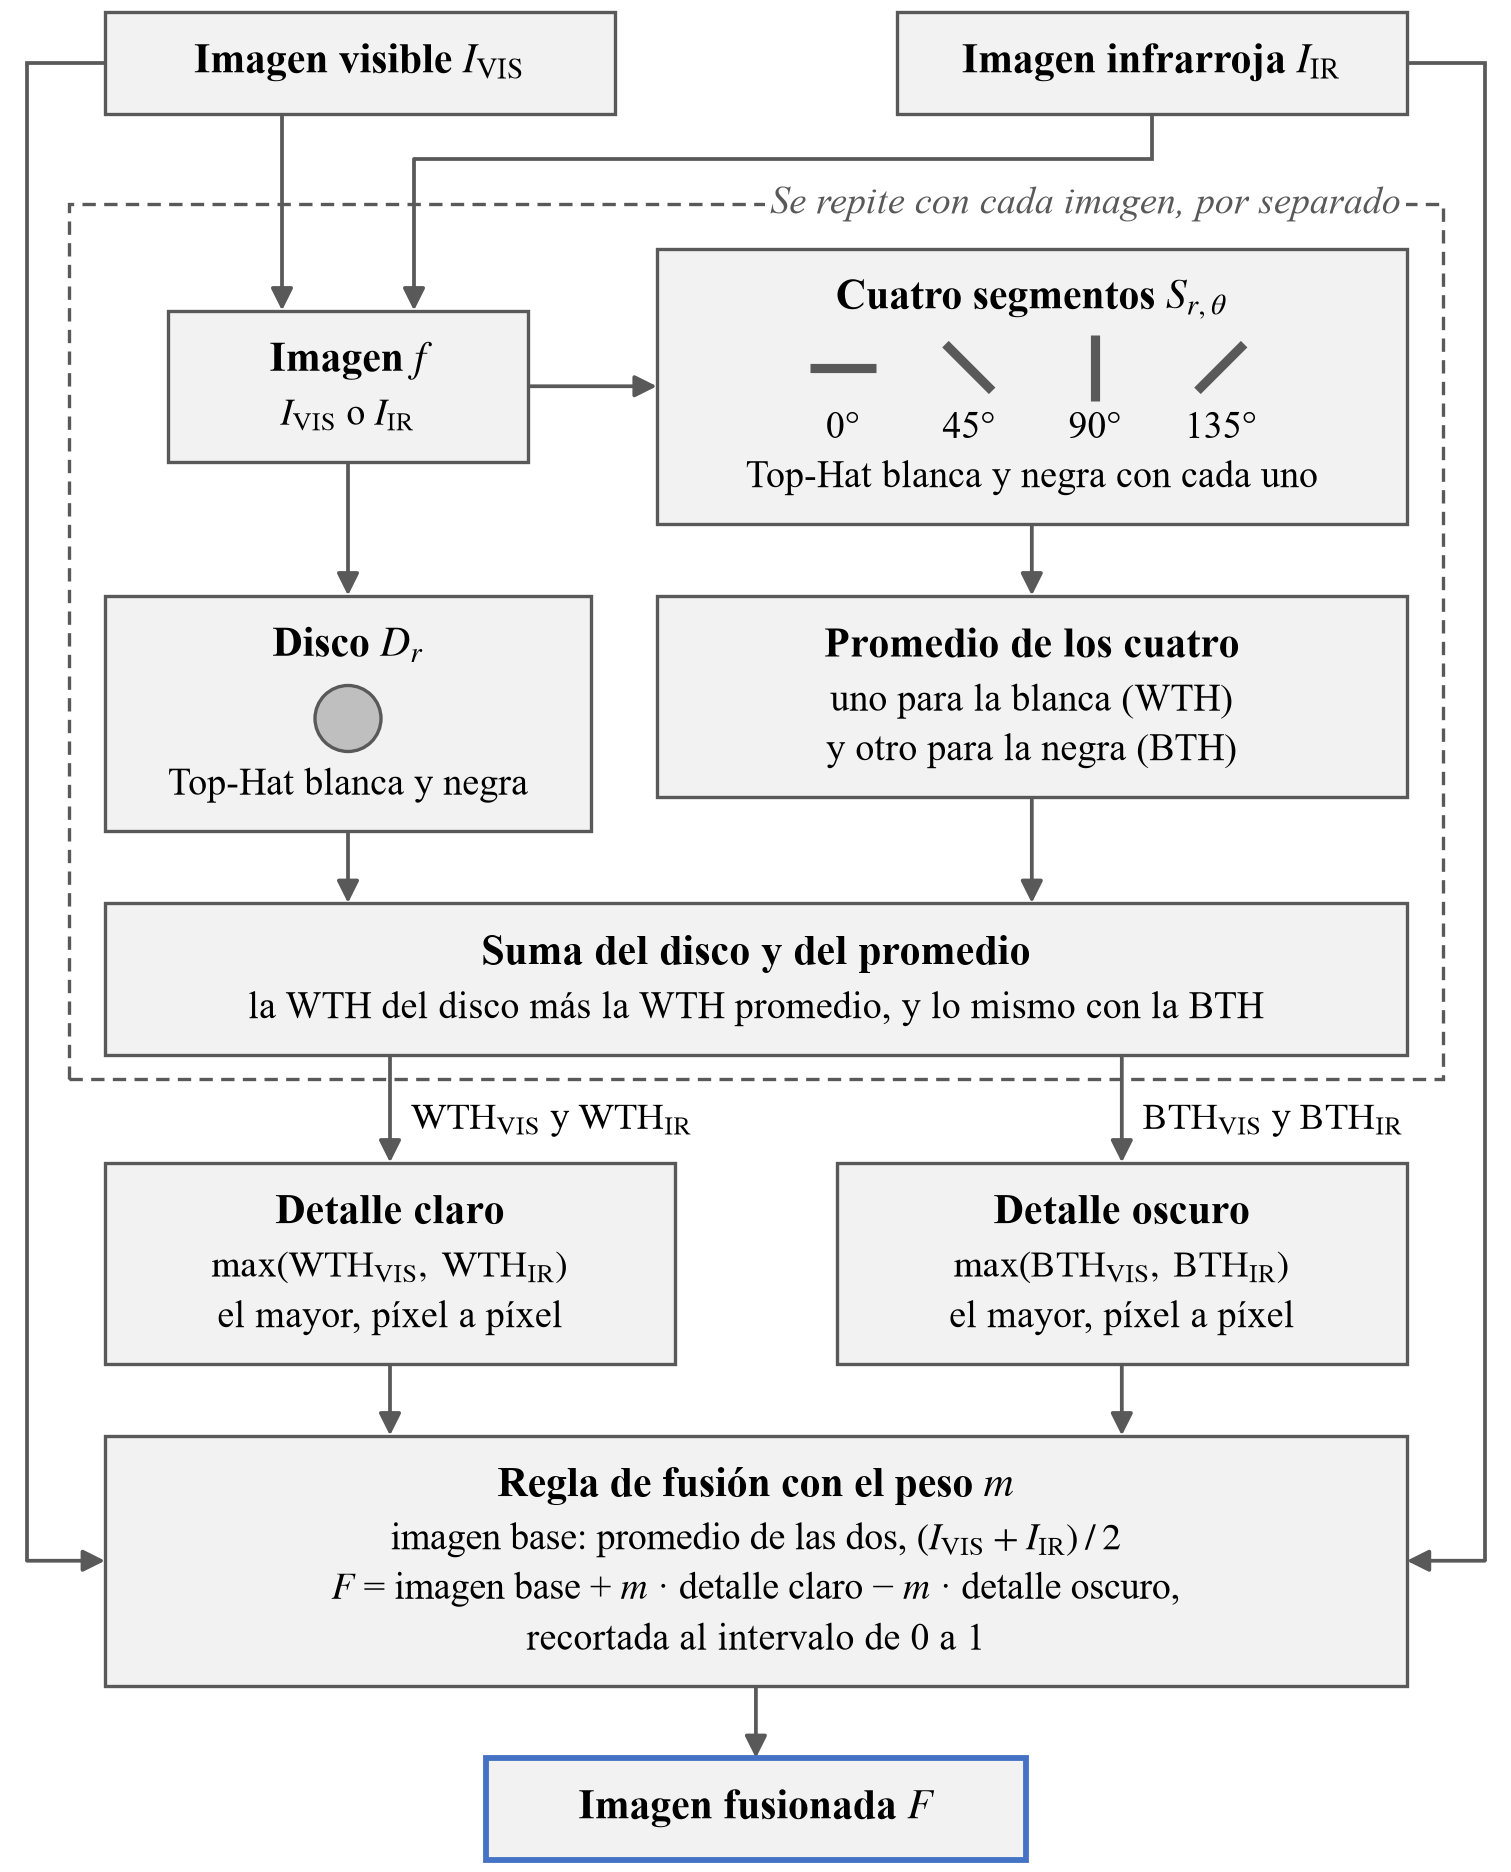
\includegraphics[width=0.8\textwidth]{figuras/fig_flujo_propuesta}
\nota{Elaboración propia. El recuadro de línea discontinua se recorre dos veces, una con la imagen
visible y otra con la infrarroja; en cada pasada, $f$ es la imagen que se procesa. Los elementos $D_r$
y $S_{r,\theta}$ se definen en las Ecuaciones~\eqref{eq:disco} y~\eqref{eq:segmentos}; WTH y BTH son las
transformadas de la Ecuación~\eqref{eq:wth-bth}. Las líneas de los costados llevan las dos imágenes de
entrada directamente a la imagen base, sin pasar por el recuadro. En la configuración adoptada, $r = 25$
y $m = 0.30$.}
\end{figure}

\subsection{Implementación y métodos comparativos}
\label{sec:operador}

La propuesta se comparó con seis métodos: el Top-Hat clásico, presentado en la
Sección~\ref{sec:fusion-tophat}, y los cinco multiescala de la Sección~\ref{sec:comparativos}. Sus
parámetros fueron los siguientes:
\begin{itemize}
\item \textbf{Top-Hat clásico:} Sigue la fusión con Top-Hat de \textcite{bajacfigueredo2024}, quienes
ensayaron elementos estructurantes de tamaños 3, 5, 7 y 9. Aquí se usa, sin ajuste, un único disco de
radio 5, es decir, de 11 píxeles de ancho, y la regla de la Ecuación~\eqref{eq:regla-tophat} con peso 1. Con ese peso, la regla agrega todo el detalle
extraído, como el realce clásico de la Ecuación~\eqref{eq:realce}.
\item \textbf{Pirámide de Laplace:} Cuatro niveles ($K = 4$), con la actividad suavizada en una ventana
de $5 \times 5$ píxeles que pesa más el centro.
\item \textbf{Pirámide de razón:} Cuatro niveles ($K = 4$), con las copias $G_0$ a $G_4$ y
$\eta = 10^{-6}$.
\item \textbf{DWT (Haar) y DWT (db4):} Tres niveles de descomposición.
\item \textbf{DTCWT:} Cuatro niveles de descomposición.
\end{itemize}
Los cinco métodos multiescala se usaron con esos parámetros, que son sus valores por defecto, sin
ajustarlos a este corpus. El Top-Hat clásico tampoco se ajustó. Entre la propuesta y el Top-Hat clásico
cambian a la vez los elementos estructurantes, el radio y el peso. Por eso, una diferencia entre los dos
no puede atribuirse al banco por sí solo.

Todos los métodos se implementaron en Python. La morfología y las pirámides se programaron con OpenCV
\parencite{bradski2000}; las transformadas \textit{wavelet}, con PyWavelets \parencite{lee2019}, y la
DTCWT, con el paquete dtcwt. Las métricas se calcularon con NumPy \parencite{harris2020}, SciPy
\parencite{virtanen2020} y scikit-image \parencite{vanderwalt2014}. Los siete métodos recibieron las
mismas entradas y pasaron por el mismo cálculo de métricas; ningún resultado se tomó de trabajos
publicados por otros autores.

Los experimentos se ejecutaron en una computadora portátil con un procesador Intel Core i7-13620H de 16 núcleos
lógicos, 31.7 GB de memoria y una tarjeta gráfica \mbox{NVIDIA} GeForce RTX 4050. La fusión y las métricas se
calcularon en el procesador, y el entrenamiento y la evaluación de los detectores se hicieron en la
tarjeta gráfica. Las versiones de los programas fueron Python 3.11, NumPy 1.26.4, OpenCV 4.13.0, SciPy 1.17.1,
scikit-image 0.26.0, PyWavelets 1.9.0, dtcwt 0.14.0, PyTorch 2.5.1 y Ultralytics 8.4.68.

\section{Ajuste de los parámetros por enjambre de partículas}
\label{sec:ajuste}

El algoritmo tiene dos parámetros. El radio $r$ define el tamaño de los cinco elementos y, con él, el
del detalle extraído, porque solo pasan a la Top-Hat los detalles en los que los elementos no caben. El
peso $m$ regula cuánto de ese detalle se suma a la imagen base. Las transformadas no dependen de $m$:
el peso solo escala el detalle antes del recorte.

Para ajustarlos se eligió la optimización por enjambre de partículas (Sección~\ref{sec:pso}), porque
es el método con que \textcite{ortegarodriguez2025} ajustan la fusión Top-Hat visible-infrarroja. De
esa obra se adaptó la función de aptitud y se tomó el rango de búsqueda: el radio
entre 1 y 25 píxeles y el peso entre 0.30 y 2.00. Las posiciones iniciales se sortearon de manera
uniforme en ese rango, y las que salían de él durante la búsqueda se llevaron al borde. Los coeficientes de la
Ecuación~\eqref{eq:pso-velocidad} valieron $c_1 = c_2 = 1.5$. La inercia bajó en línea recta, según la
Ecuación~\eqref{eq:pso-inercia}, de $w_{\max} = 0.9$ en la primera iteración a $w_{\min} = 0.4$ en la
última. La obra de referencia también usa una inercia decreciente, pero no publica sus extremos ni los
coeficientes.

La aptitud adapta la función que esa obra llama $F_o$. El radio de cada partícula se redondea al entero
más cercano, porque los elementos se arman con un número entero de píxeles. Con el radio y el peso se
fusionan los $N$ pares del ajuste, y $F_n$ es la imagen que resulta del par $n$. La aptitud es
\begin{equation} \begin{aligned} \mathrm{Apt}(r, m) = \frac{1}{N}\sum_{n=1}^{N}\biggl[ & \frac{\mathrm{SSIM}(I_{\mathrm{VIS},n}, F_n) + \mathrm{SSIM}(I_{\mathrm{IR},n}, F_n)}{2} \\
 & + \frac{\mathrm{EN}(F_n)}{8} + \frac{\mathrm{PSNR}(F_n)}{100}\biggr]. \end{aligned} \label{eq:aptitud} \end{equation}

El primer término es la similitud estructural media con las dos fuentes. A diferencia de la métrica de
la Ecuación~\eqref{eq:met-ssim}, usa la ventana que proponen \textcite{wang2004}. Esa ventana mide
$11 \times 11$ píxeles, ponderados con una curva gaussiana de desviación estándar 1.5, y el índice se
promedia sobre todas las posiciones de la imagen. El segundo término es la entropía de la
Ecuación~\eqref{eq:met-en} dividida por 8, su máximo. El tercero es la PSNR de la
Ecuación~\eqref{eq:met-psnr} dividida por 100. De los tres términos, dos premian el parecido con las
fuentes y solo la entropía premia la información de la imagen.

La obra de referencia ajusta los parámetros escena por escena. Aquí, en cambio, se buscó una sola
configuración, con la aptitud evaluada sobre tres escenas: dos con vehículos blindados y una con un
soldado detrás de una cortina de humo. De cada escena se tomó un par, y los tres pares forman parte de
los veinte con que se evaluó la calidad. El ajuste comprendió estos ensayos:
\begin{itemize}
\item \textbf{Configuraciones del enjambre:} Veinticinco corridas que, como en la obra de referencia,
cruzan cinco cantidades de partículas (2, 4, 6, 8 y 10) con cinco de iteraciones (10, 20, 30, 40 y 50).
\item \textbf{Repeticiones:} Como control de la variación al azar, las veinticinco configuraciones se
repitieron veinte veces, lo que da quinientas corridas en total.
\item \textbf{Grilla:} La aptitud se calculó en cinco mil combinaciones, que cruzan los veinticinco
radios con doscientos pesos de 0.01 a 2.00. La grilla incluye pesos menores que 0.30, fuera del rango
de búsqueda.
\item \textbf{Barrido del peso:} En las mismas tres escenas, las seis métricas se calcularon con once
pesos, de 0.05 a 2.0. El barrido abarcó la propuesta con $r = 25$ y el Top-Hat clásico con $r = 5$ y
con $r = 25$.
\end{itemize}

Como las corridas pueden terminar en radios distintos, la configuración se eligió entre los dos radios
a los que llegaron más corridas. Esos dos candidatos se compararon sobre los veinte pares del corpus
con las nueve métricas iniciales (Sección~\ref{sec:metricas}), con prioridad para las de
actividad, que reflejan el realce. La comparación usó las mismas imágenes con que después se evaluó la
calidad, una limitación que señala la Sección~\ref{sec:limitaciones}. La configuración adoptada fue
$r = 25$ y $m = 0.30$. Ese radio es uno de los dos resultados del enjambre, y se lo adoptó porque
prioriza el realce. La Sección~\ref{sec:res-ajuste} informa en qué radios y pesos terminaron las
corridas.

\section{Protocolo de evaluación de la calidad de imagen}
\label{sec:protocolo-calidad}

Como la fusión visible-infrarroja no dispone de una imagen ideal con la cual comparar el resultado, la
calidad se midió con seis métricas sin referencia, presentadas en la Sección~\ref{sec:metricas}. Tres
son de actividad y miden la información, el contraste y la nitidez de la imagen. Las otras tres son de
fidelidad y miden cuánto se parece la fusión a sus fuentes. La Tabla~\ref{tab:metricas} las resume.

\begin{table}[htbp]
\centering
\caption{Las seis métricas de evaluación de calidad}
\label{tab:metricas}
\setlength{\tabcolsep}{4pt}
\begin{tabular}{@{}lll@{}}
\toprule
\textbf{Métrica} & \textbf{Qué mide} & \textbf{Grupo} \\
\midrule
Entropía (EN)                        & cantidad de información de la imagen   & actividad \\
Desviación estándar (SD)             & contraste general                      & actividad \\
Gradiente medio (MG)                 & nitidez de los bordes                  & actividad \\
Información mutua (MI)               & cuánto de las fuentes se conserva      & fidelidad \\
Similitud estructural (SSIM)         & parecido estructural con las fuentes   & fidelidad \\
Relación señal-ruido de pico (PSNR)  & fidelidad numérica a las fuentes       & fidelidad \\
\bottomrule
\end{tabular}
\nota{Elaboración propia. Las métricas de actividad se calculan solo con la imagen fusionada, y las de
fidelidad la comparan con sus fuentes.}
\end{table}

Las seis surgen de depurar una batería inicial de nueve con dos criterios: no repetir información y
equilibrar los dos grupos. De esas nueve, las de actividad eran EN, SD, FE, MG y SF, y las de
fidelidad, la MI con cada fuente, la SSIM y la PSNR. Como comprobación, la
clasificación se repitió con esas nueve y con diecisiete: las mismas más las ocho métricas
complementarias de la Sección~\ref{sec:metricas}.

Equilibrar los grupos no impide que el ruido reciba premio, porque el ruido también eleva la actividad
de una imagen. Para medir ese efecto se agregó un control con el promedio simple y versiones degradadas
de él:
\begin{itemize}
\item \textbf{Promedio simple:} La media píxel a píxel de la visible y la infrarroja, sin detalle
agregado.
\item \textbf{Promedio con ruido:} El promedio simple con ruido gaussiano de desviación estándar 0.02,
0.05, 0.10 y 0.20.
\item \textbf{Promedio desenfocado:} El promedio simple suavizado con núcleos gaussianos de
$5 \times 5$ y de $11 \times 11$ píxeles.
\end{itemize}
Esas siete versiones de cada par se ordenaron junto con los siete métodos de fusión, con las mismas seis
métricas. Si una imagen con ruido sube en la clasificación, una actividad alta no basta para probar que
el detalle agregado sea útil.

El análisis estadístico fue no paramétrico. Con veinte pares no podía suponerse que las métricas
siguieran una distribución normal, y lo que interesaba era el orden entre los métodos. Para cada métrica
se aplicó primero la prueba de Friedman \parencite{friedman1937}, con cada par de imágenes como bloque.
Cuando resultó significativa, se aplicó la prueba de Wilcoxon de rangos con signo
\parencite{wilcoxon1945} a once contrastes entre pares de métodos. La propuesta se enfrentó con el
Top-Hat clásico y con cada uno de los cinco multiescala, y el Top-Hat clásico, con esos mismos cinco.
Los valores de $p$ se corrigieron con el procedimiento de Holm \parencite{holm1979} dentro de cada
métrica.

Cada contraste se resumió en uno de tres desenlaces. Si el valor de $p$ corregido era menor que 0.05,
contaba como victoria o como derrota, según el signo de la diferencia de medias entre los dos métodos.
Si no lo era, contaba como empate. Con seis métricas, el análisis reúne sesenta y seis decisiones de
este tipo.

Para resumir el desempeño se usó la clasificación por rango promedio. Dentro de cada par se ordenaron
los siete métodos según cada métrica, con el rango medio en caso de empate. Esos puestos se promediaron
luego sobre los pares y las métricas, y un valor más bajo indica un método mejor ubicado. El
procedimiento respeta la estructura en bloques del experimento y evita promediar magnitudes de unidades
distintas. El cálculo se repitió por separado con las métricas de actividad y con las de fidelidad, lo
que da el perfil de cada método. El rango promedio no tiene una prueba propia y se lee de forma
descriptiva.

Las pruebas tratan los veinte pares como bloques independientes, pero once de ellos provienen de solo
cuatro escenas. Para ver si esa dependencia alteraba las conclusiones, el análisis completo se repitió
con trece bloques, uno por escena. En cada escena con varias tomas, las métricas se promediaron sobre
ellas.

La evaluación se completó con una comparación visual de dos escenas, que es solo ilustrativa. Se las
eligió porque muestran dos maneras distintas en que las cámaras se complementan. En la primera, una
persona apenas se distingue en la imagen visible nocturna. En la segunda, una cortina de humo le oculta
la escena a la cámara visible. Esta segunda escena es una de las tres que se usaron en el ajuste de los
parámetros.

\section{Aplicación a la detección de objetos}
\label{sec:protocolo-deteccion}

En la aplicación que se estudia, la imagen fusionada alimenta un detector automático de objetos. La
pregunta es si, con ella, el detector encuentra lo que cada cámara ve por separado. Como un detector
aprende la apariencia de sus imágenes de entrenamiento, se entrenaron detectores propios para cada tipo
de imagen, según la práctica de \textcite{liu2022}, descrita en la Sección~\ref{sec:marco-deteccion}. Hubo diez
entradas: la visible, la infrarroja, el promedio simple y las siete fusiones. Todas usaron los mismos cuadros, las mismas
etiquetas y la misma configuración del detector.

\subsection{Partición de los datos}
\label{sec:det-datos}

Las imágenes de M3FD son cuadros de secuencias de video, y los cuadros vecinos se parecen mucho entre
sí. Si un cuadro de prueba tuviera un vecino casi idéntico en el entrenamiento, el detector se evaluaría
sobre algo que ya vio. Para evitarlo, los cuadros se agruparon en bloques de cien números de cuadro
consecutivos, y los bloques se cortaron también donde cambia el tamaño de la imagen. Los bloques,
enteros, se sortearon hasta reunir cerca del 25~\% de los cuadros para la prueba y del 10~\% para la
validación, y el resto fue al entrenamiento. Se tomó el primer sorteo que dejaba en la prueba entre el
20 y el 35~\% de las personas y de las luces. Donde se tocaban bloques de partes distintas, se
descartaron diez cuadros a cada lado del límite, 496 en total.

De los bloques de entrenamiento se tomaron al azar 2000 cuadros para entrenar. Los 474 restantes, que
aquí se llaman cuadros de seguimiento, se reservaron para seguir el entrenamiento y calibrar el umbral
de confianza. Los bloques de validación no intervinieron en el entrenamiento ni en ninguna elección, y
se sumaron a la prueba. Sobre la prueba se aplicaron luego dos filtros:
\begin{itemize}
\item \textbf{Casi duplicados en la visible:} En la imagen visible, cada cuadro se comparó con los de
entrenamiento mediante la similitud estructural. Se lo descartó si con alguno alcanzaba la mediana de
esa similitud entre cuadros consecutivos. Este filtro sacó 33 cuadros, todos de los bloques de prueba, y
dejó 1197.
\item \textbf{Parecido en las dos cámaras:} Cada cuadro se comparó también con los de entrenamiento
mediante la correlación, en la visible y en la infrarroja. Se lo descartó si, con un mismo cuadro de
entrenamiento, alcanzaba en ambas a la vez el primer cuartil de esa medida entre cuadros
consecutivos. Este filtro sacó otros 130.
\end{itemize}
La prueba final quedó en 1067 cuadros, con 2045 personas y 864 luces marcadas. Sus bloques se unieron
cuando eran contiguos, y así se formaron once grupos. En la inferencia, la unidad independiente fue el
grupo y no el cuadro, porque los cuadros de un mismo tramo de video no son independientes entre sí.

\subsection{Detector y entrenamiento}
\label{sec:det-detector}

El detector fue YOLOv8 \parencite{jocher2023} en su variante más pequeña, YOLOv8n, con la biblioteca
Ultralytics 8.4.68. Cada detector partió de los pesos con que se distribuye la red YOLOv8n,
entrenados sobre las fotografías comunes del conjunto de \textcite{lin2014}. Se lo entrenó con las seis
clases de M3FD y los 2000 cuadros de entrenamiento durante cuarenta épocas, es decir, cuarenta pasadas
completas por esos cuadros. Las imágenes se procesaron a 640 píxeles de lado, en lotes de dieciséis.
Los pesos de la red se actualizaron con el algoritmo AdamW \parencite{loshchilov2019}, con una tasa de
aprendizaje de 0.001 y un momento de 0.9. El detector se evaluó tal como quedó al final, sin elegir
ninguna época intermedia.

Para cada entrada se entrenaron tres detectores, con tres semillas distintas, y se obtuvieron así
treinta en total. La semilla fija las elecciones aleatorias del entrenamiento, entre ellas el orden de
las imágenes en los lotes y las transformaciones que se les aplican al azar. Cambiarla introduce, por lo
tanto, una variación ajena al método de fusión, que la repetición del entrenamiento permite estimar. Los detectores de la visible y
de la infrarroja se entrenaron con semillas propias, distintas de las que usaron el promedio simple y las
siete fusiones. Solo el primero de los tres entrenamientos de cada entrada se siguió época por época,
con la mAP50 sobre los cuadros de seguimiento.

\subsection{Objetos de una sola cámara y tasa de acierto equilibrada}
\label{sec:det-medida}

De las seis clases, el análisis se centró en las personas y las luces, porque su visibilidad en las dos
cámaras es opuesta. Una persona se destaca en la imagen térmica aunque esté a oscuras; una luz
encendida, en la visible. Los detectores entrenados con cada cámara lo reflejan en los 1197 cuadros que
dejó el primer filtro. En personas, la precisión media AP50 fue de 0.697 con la infrarroja y de 0.431
con la visible. En luces fue de 0.124 con la visible y de 0.020 con la infrarroja. Entre las seis
clases, la de personas es la que muestra la mayor ventaja de la infrarroja sobre la visible, y la de
luces, la mayor ventaja de la visible sobre la infrarroja.

Un objeto marcado cuenta como encontrado si el detector predice su clase con una confianza igual o
mayor que el umbral y una IoU de al menos 0.5 (Ecuación~\ref{eq:iou}). Un objeto es de una sola
cámara si lo encuentran al menos dos de los tres detectores de esa cámara y a lo sumo uno de los tres de
la otra. Si lo encuentran al menos dos de los tres detectores de cada cámara, es un objeto de las dos.

La medida principal es la tasa de acierto equilibrada. Es el promedio de dos tasas: la de acierto sobre
los objetos de solo la visible y la de acierto sobre los de solo la infrarroja. Así, ninguno de los dos
tipos de objeto pesa más por ser más numeroso. Para cada entrada, un objeto aporta la fracción de los
tres detectores de esa entrada, uno por semilla, que lo encuentran. Las tasas de la visible y de la infrarroja no
se informan, porque sus detectores son los que definen los objetos.

La confianza de cada detector tiene su propia escala, de modo que un mismo umbral no pone a todos en
igualdad de condiciones. Por eso el umbral principal se calibró detector por detector. Como referencia
se tomó la cantidad de falsos positivos de personas y luces que, en promedio, cometen por imagen los
detectores de la visible con un umbral de 0.25. A cada detector se le asignó, entre los umbrales de 0.05 a 0.95 en pasos de 0.01,
el umbral con que comete la cantidad más cercana a esa. La calibración se hizo sobre los cuadros de seguimiento, nunca sobre la prueba. Para el
análisis de sensibilidad se usaron el umbral fijo de 0.25 y el umbral de mejor equilibrio por clase. Este último
maximiza, en cada clase, la media armónica de la precisión y la exhaustividad en esos mismos cuadros.

\subsection{Comparación con el Top-Hat clásico y medidas secundarias}
\label{sec:det-comparacion}

La comparación central resta a la tasa equilibrada de la propuesta la del Top-Hat clásico, y expresa la
diferencia en puntos porcentuales. Su intervalo de confianza del 95~\% toma como unidad cada grupo de
cuadros y no cada objeto, porque los objetos de un mismo tramo de video no son independientes. Se lo
calculó con un error estándar robusto por grupos y con la distribución $t$. Sus grados de libertad
equivalen a la cantidad de grupos con objetos de una sola cámara, menos uno \parencite{cameron2015}.

Tres análisis de sensibilidad revisaron la solidez de esa diferencia:
\begin{itemize}
\item \textbf{\textit{Bootstrap} salvaje por grupos:} Se generan 9999 réplicas con la hipótesis nula
impuesta. En cada una, los residuos de cada grupo se multiplican por un peso sorteado entre seis valores
fijos, y el estadístico $t$ de la réplica se compara con el observado \parencite{cameron2008, webb2023}.
El intervalo reúne las diferencias que esta prueba no rechaza al 5~\%.
\item \textbf{Otros umbrales:} La diferencia y su intervalo se recalculan con el umbral fijo de 0.25 y
con el de mejor equilibrio por clase.
\item \textbf{Pares de semillas:} Con tres semillas por entrada hay nueve combinaciones de un detector
de la propuesta con uno del Top-Hat clásico, y cada una da su propia diferencia. La comparación se
considera robusta a la semilla si las nueve diferencias tienen el mismo signo.
\end{itemize}
Las tasas de las demás entradas, entre ellas el promedio simple y los cinco métodos multiescala, se
informan de manera descriptiva, como referencia. La diferencia entre la propuesta y el promedio simple
se calculó, además, con el mismo intervalo por grupos. Como el promedio simple es la regla de la
Ecuación~\eqref{eq:regla-tophat} con peso cero, esa diferencia estima el aporte del detalle agregado.
También se informa como referencia y no forma parte del examen de la hipótesis.

Se calcularon, además, cuatro medidas secundarias:
\begin{itemize}
\item \textbf{Precisión media global:} La mAP50 de la Ecuación~\eqref{eq:map50}, sobre las seis clases
y los 1197 cuadros que dejó el primer filtro, promediada sobre las tres semillas. Se la calculó sin
aplicar el segundo filtro, de modo que incluye los 130 cuadros que este descartó, y no interviene en el
examen de la hipótesis.
\item \textbf{Objetos de las dos cámaras:} La tasa de acierto sobre los objetos que encuentran a la vez
los detectores de la visible y los de la infrarroja.
\item \textbf{Cuadros con un objeto de cada cámara:} En los cuadros con al menos un objeto de solo la
visible y uno de solo la infrarroja, la fracción en que el detector encuentra al menos uno de cada tipo.
\item \textbf{Relación entre calidad y detección:} Para los siete métodos de fusión, la correlación de
rangos de Spearman \parencite{spearman1904} entre su rango promedio de calidad y su tasa equilibrada.
\end{itemize}
En estas medidas, las diferencias entre métodos no se sometieron a prueba.

\section{Examen de la hipótesis}
\label{sec:examen-hipotesis}

La hipótesis del trabajo, enunciada en el Capítulo~\ref{cap:introduccion}, reúne tres afirmaciones: dos
sobre la calidad de imagen y una sobre la aplicación a la detección. Cada una se examinó con las pruebas
de su evaluación, sin agregar otras:
\begin{itemize}
\item \textbf{Mejor calidad que el Top-Hat clásico:} Se usaron los seis contrastes de Wilcoxon contra
el Top-Hat clásico, uno por métrica, con la corrección de Holm. Un contraste significativo al 5~\%
contó como victoria o como derrota, según el signo de la diferencia, y uno no significativo, como
empate. El reparto se informa tal como resulta, con el rango promedio de los dos métodos como
complemento.
\item \textbf{Calidad comparable a la de los cinco métodos multiescala:} Se usaron el rango promedio con
las seis métricas y el perfil de la propuesta. El perfil reúne sus contrastes contra cada uno de los
cinco y su puesto en actividad y en fidelidad. Como el rango promedio no tiene una prueba propia y
depende de las métricas elegidas, se lo leyó junto con las clasificaciones de nueve y de diecisiete
métricas. Esta afirmación se examinó, por lo tanto, de forma descriptiva.
\item \textbf{Más objetos de una sola cámara que el Top-Hat clásico:} La afirmación se sostiene si, con
el umbral principal, el límite inferior del intervalo de confianza con la distribución $t$ supera el
cero. Se revisaron además los otros dos umbrales, el \textit{bootstrap} salvaje por grupos y los nueve
pares de semillas. Si la diferencia no resulta robusta a la semilla, se la informa como un hallazgo por
confirmar, aunque se cumpla esa condición.
\end{itemize}

En la detección, la propuesta se comparó solo con el Top-Hat clásico porque pertenece a la misma
familia y usa la misma regla de fusión (Ecuación~\ref{eq:regla-tophat}). La comparación mide, así, el
efecto de cambiar el operador en su conjunto, con sus elementos, su radio y su peso
(Sección~\ref{sec:operador}).

\chapter{Resultados}
\label{cap:resultados}

Este capítulo presenta los resultados en el orden general en que el Capítulo~\ref{cap:metodologia}
describió los procedimientos. Primero se describen los dos conjuntos de imágenes y el ajuste de los
parámetros. Siguen la comparación visual, las mediciones de calidad y su análisis estadístico, y después
la aplicación a la detección de objetos. La última sección reúne los resultados con que se examina la
hipótesis. El capítulo los informa sin discutirlos; la discusión queda para el
Capítulo~\ref{cap:discusion}.

\section{Caracterización de los conjuntos}
\label{sec:caracterizacion}

Los veinte pares del TNO con que se evaluó la calidad provienen de trece escenas. Tres escenas aportan
tres tomas cada una, otra aporta dos y las nueve restantes, una sola. Así, once pares se concentran en
cuatro escenas, y por eso el análisis estadístico se repitió con un bloque por escena
(Sección~\ref{sec:res-robustez}). Diecisiete pares pertenecen a la colección Athena y tres a la
colección Triclobs.

Las imágenes no tienen todas el mismo tamaño. Entre los veinte pares aparecen once resoluciones, desde
$359 \times 247$ hasta $768 \times 576$ píxeles, y la mayor es también la más frecuente, con nueve
pares. Dentro de cada par, la imagen visible y la infrarroja tienen el mismo tamaño, de modo que ninguna
debió redimensionarse.

En M3FD, la prueba de detección quedó formada por 1067 cuadros con 2045 personas y 864 luces, repartidos
en once grupos de bloques contiguos (Sección~\ref{sec:det-datos}). Las luces no se distribuyen de forma
pareja entre esos grupos: aparecen solo en cinco de ellos, y uno reúne 555 de las 864, el 64.2~\%, casi
dos de cada tres.

\section{Ajuste de los parámetros}
\label{sec:res-ajuste}

Las corridas del enjambre coincidieron en el peso, pero no en el radio. Las veinticinco, una por
configuración, terminaron con $m = 0.30$, el límite inferior del rango de búsqueda. En cambio, dieciséis
terminaron en $r = 1$, ocho en $r = 25$ y una en $r = 14$. La aptitud, la función que el enjambre
optimiza, fue de 1.7350, 1.7057 y 1.6990 en esos tres resultados, respectivamente. El panel (b) de la
Figura~\ref{fig:ajuste_pso} muestra ese reparto de los radios, y el panel (a), cómo cambia la aptitud
con el peso en $r = 1$ y en $r = 25$.

\begin{figure}[htbp]
\centering
\caption{Aptitud según el peso $m$ y reparto de las corridas del enjambre por radio final}
\label{fig:ajuste_pso}
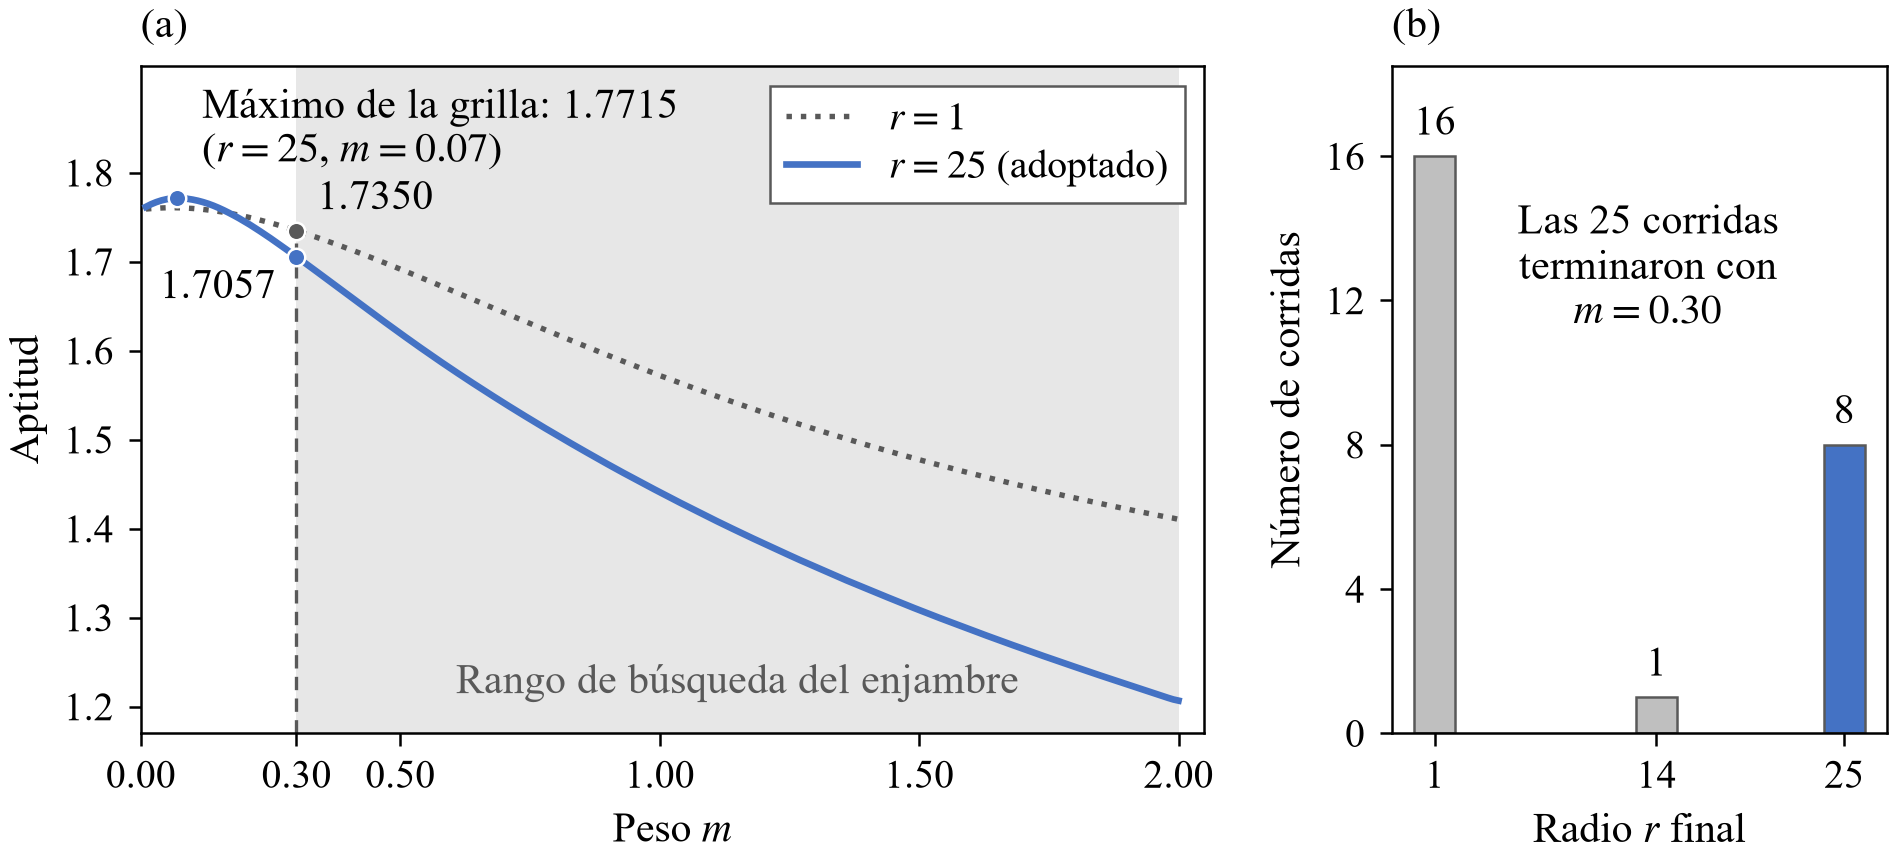
\includegraphics[width=\textwidth]{figuras/fig_ajuste_pso}
\nota{Elaboración propia. (a) Aptitud de la propuesta (Ecuación~\ref{eq:aptitud}) sobre las tres
escenas del ajuste, en función del peso $m$, con los radios $r = 1$ (gris, línea punteada) y $r = 25$
(azul, línea continua). Las
curvas se trazaron con los valores de la grilla, que recorre los pesos de 0.01 a 2.00 cada 0.01. La zona sombreada es
el rango de búsqueda del enjambre, de 0.30 a 2.00, y la línea discontinua marca $m = 0.30$. Los rótulos
indican la aptitud de cada radio en ese peso y el máximo de la grilla. (b) Número de corridas del enjambre
que terminaron en cada radio, de un total de veinticinco, una por configuración de partículas e
iteraciones. En azul está el radio adoptado.}
\end{figure}

Las quinientas corridas de control, que repitieron cada configuración para medir la variación al azar,
mostraron el mismo patrón. En 499 de ellas, el 99.8~\%, el peso terminó en 0.30, y en la restante, en
0.36. El radio volvió a dividirse entre los dos extremos del rango: el
51.4~\% de las corridas terminó en $r = 25$, el 45.6~\% en $r = 1$ y el 3.0~\% restante en otros
radios.

La grilla de cinco mil combinaciones de radio y peso, de la que sale el panel (a), muestra la forma de
la aptitud. Su máximo, 1.7715, se dio en $r = 25$ y $m = 0.07$, fuera del rango de búsqueda.
En cada radio, el mejor peso estuvo entre 0.05 y 0.07, y en los veinticinco radios la aptitud bajó en
cada paso del peso a partir de $m = 0.30$. Dentro del rango de búsqueda, la mayor aptitud fue la de
$r = 1$ y $m = 0.30$, el punto al que llegaron dieciséis corridas. Con el peso en 0.30, la aptitud presentó dos
máximos locales en el radio: uno en $r = 1$, el mayor, y otro en $r = 25$.

Como las corridas se repartieron entre $r = 1$ y $r = 25$, los dos radios se compararon sobre los veinte
pares del corpus, con $m = 0.30$ y las nueve métricas iniciales. El radio 25 fue mejor en las de
actividad, que miden información, contraste y nitidez, y peor en las de fidelidad, que miden el parecido
con las fuentes. Las cinco de actividad son la entropía, la desviación estándar, la eficiencia de
fusión, el gradiente medio y la frecuencia espacial. En cada una, el radio mayor superó a $r = 1$ en los
veinte pares. Las cuatro de fidelidad son la información mutua con cada fuente, la similitud estructural y la
relación señal-ruido de pico. En cada una de estas, $r = 1$ quedó por delante en diecinueve o en veinte
pares.

Con las seis métricas del trabajo, el patrón fue el mismo: $r = 25$ obtuvo valores mayores en las tres
de actividad y menores en las tres de fidelidad. Al pasar de $r = 1$ a $r = 25$, la desviación estándar media subió
de 0.1092 a 0.1439 y el gradiente medio, de 0.0234 a 0.0355. En sentido contrario, la similitud
estructural bajó de 0.7484 a 0.6584 y la información mutua, de 0.9670 a 0.7486. Se adoptó
$r = 25$, uno de los dos resultados del enjambre, porque prioriza el realce. La configuración de la
propuesta que se evalúa en el resto del capítulo es, entonces, $r = 25$ y $m = 0.30$.

El barrido del peso sobre las tres escenas del ajuste mostró que, al aumentar $m$, las métricas de
actividad subieron y las de fidelidad bajaron, con una sola excepción en la propuesta. Con la propuesta
en $r = 25$, la desviación estándar y el gradiente medio subieron en cada paso, desde $m = 0.05$ hasta
$m = 2.0$. La información mutua, la similitud estructural y la relación señal-ruido de pico, en cambio,
bajaron en cada paso. La excepción fue la entropía, que subió hasta $m = 1.2$ y luego descendió. En el
Top-Hat clásico, tanto con $r = 5$ como con $r = 25$, no hubo excepciones: las tres métricas de
actividad subieron y las tres de fidelidad bajaron en cada paso.

\section{Comparación cualitativa}
\label{sec:cualitativa}

Las Figuras~\ref{fig:montaje_kaptein} y~\ref{fig:montaje_humo} presentan dos escenas del corpus, cada
una con sus dos fuentes y las imágenes de los siete métodos. Muestran dos maneras en que las cámaras se
complementan. En la primera, la cámara visible casi no capta a una persona. En la segunda, una
cortina de humo oculta la escena a la cámara visible, y solo la térmica la atraviesa. La comparación es
ilustrativa y no sostiene conclusiones por sí misma.

\begin{figure}[htbp]
\centering
\caption{Fuentes y fusiones de una escena nocturna del TNO (Kaptein 1123)}
\label{fig:montaje_kaptein}
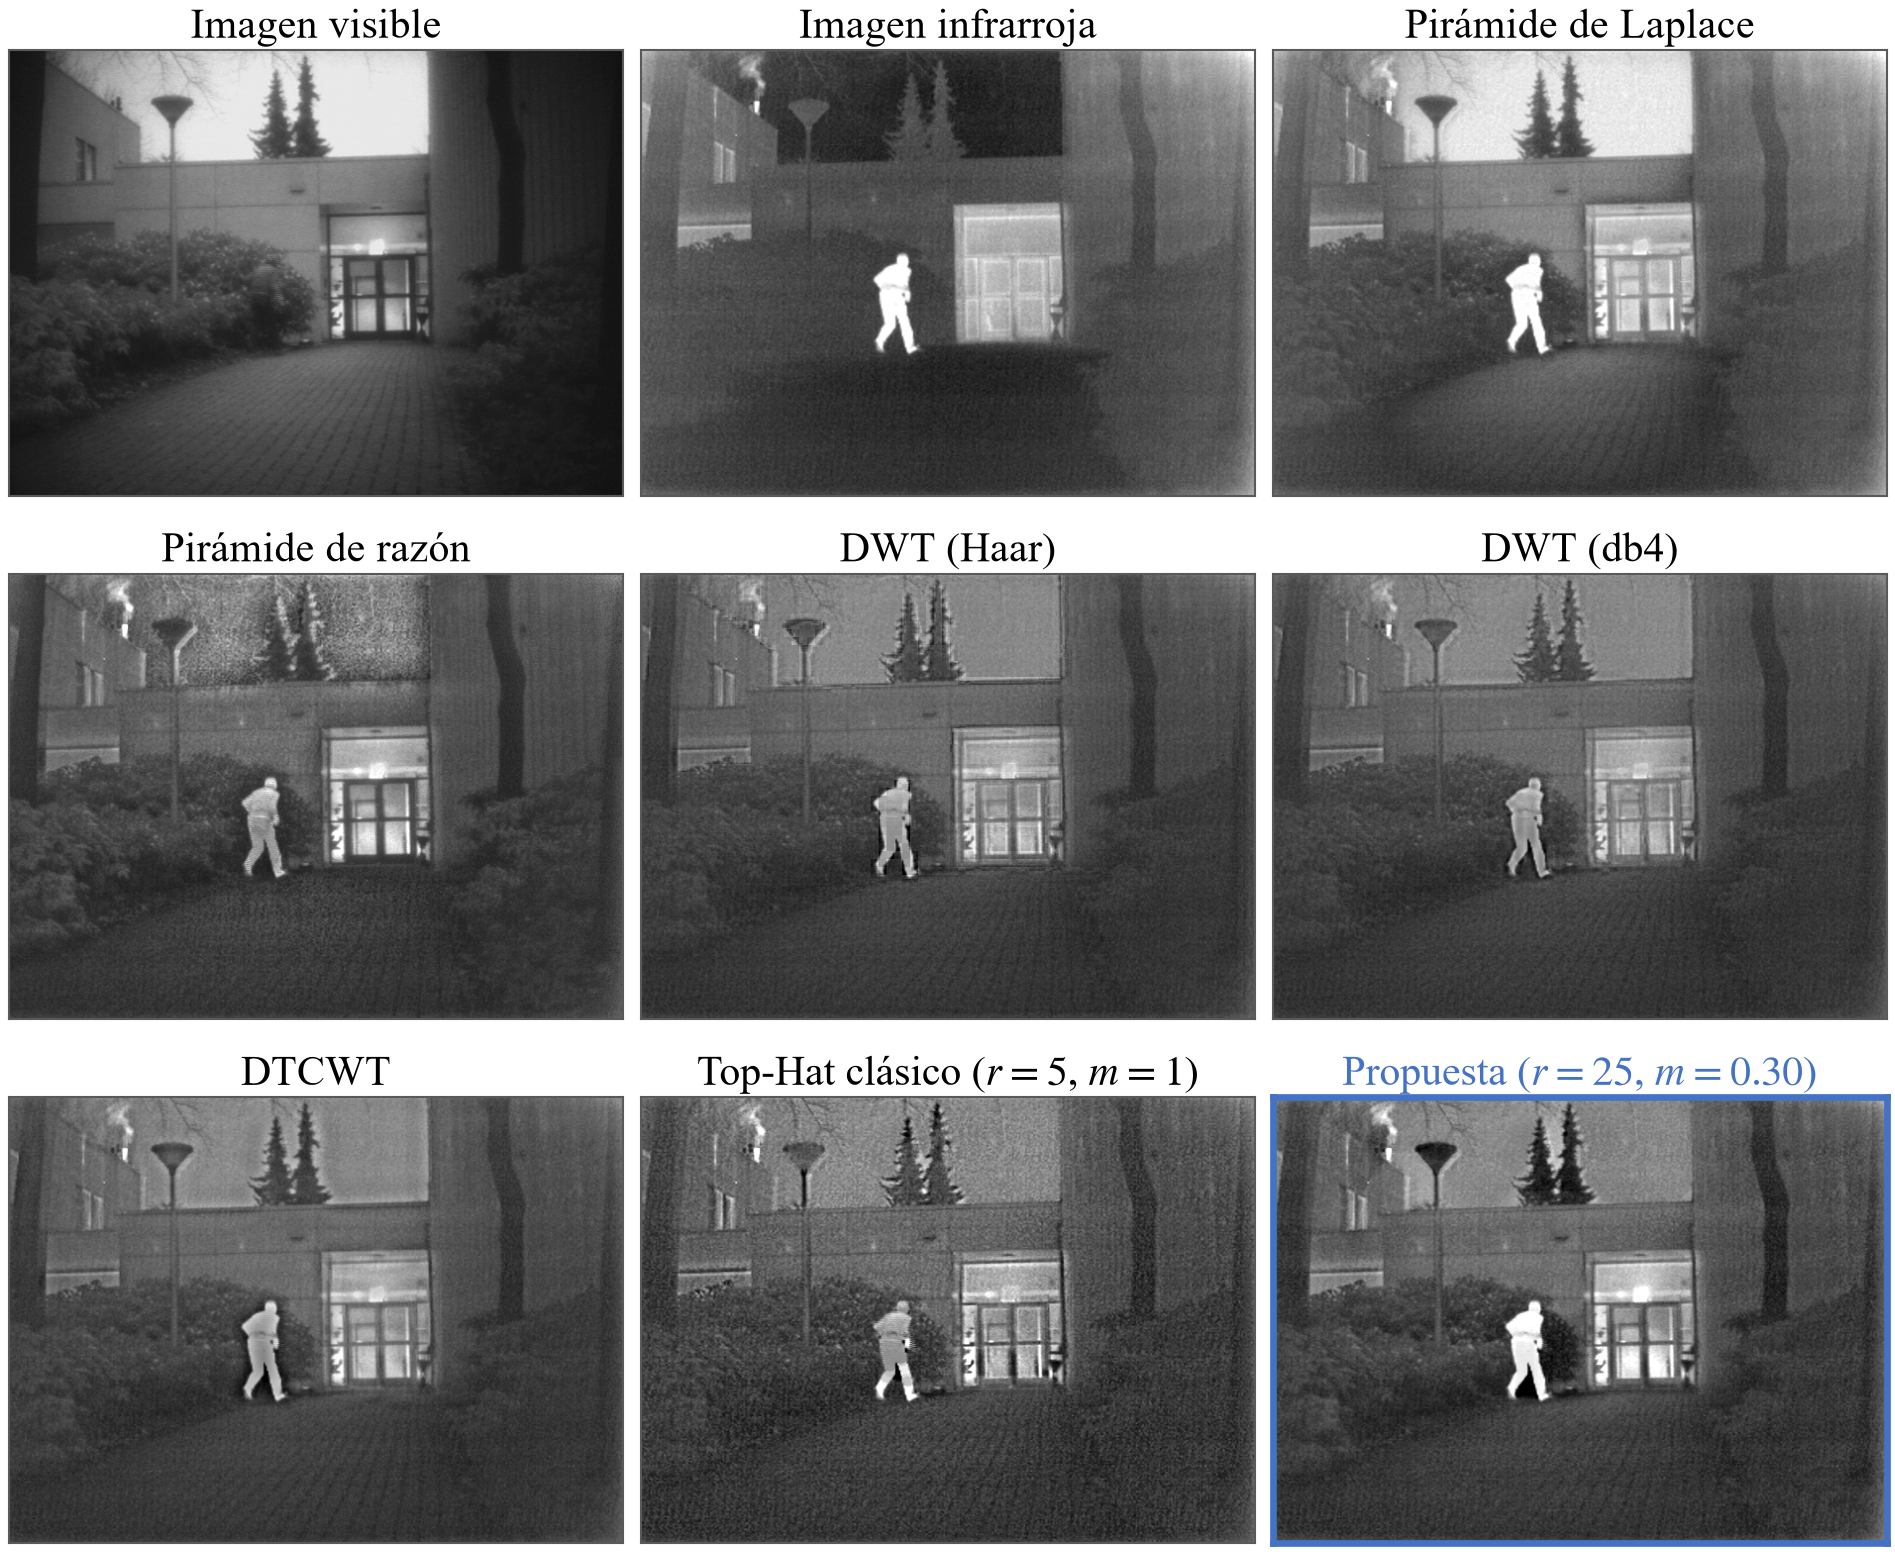
\includegraphics[width=\textwidth]{figuras/montaje_kaptein}
\nota{Elaboración propia a partir de imágenes del \textit{TNO Image Fusion Dataset} \parencite{toet2014, toet2017}. En
la escena hay una persona que en la imagen visible casi no se distingue del fondo. Las dos primeras
imágenes son las fuentes, y las siete siguientes, en orden de lectura, las fusiones de cada método. La
fusión de la propuesta está recuadrada en azul.}
\end{figure}

En la escena nocturna, la imagen visible deja ver con nitidez el edificio, el farol, los árboles y el
sendero de adoquines. La persona que avanza por el sendero, en cambio, se confunde con los arbustos
oscuros. En la infrarroja aparece como una figura brillante, pero el follaje pierde buena parte de su
textura. Las siete fusiones reunieron la silueta de la persona con el fondo de la visible. La pirámide
de razón dejó granulado el cielo, y el Top-Hat clásico, la imagen entera. La pirámide de Laplace y la
propuesta fueron las que más separaron a la persona del fondo. En la propuesta se formó, además, un
borde oscuro alrededor de la figura, con un relleno negro entre las piernas.

\begin{figure}[htbp]
\centering
\caption{Fuentes y fusiones de una escena del TNO con un soldado tendido tras una cortina de humo}
\label{fig:montaje_humo}
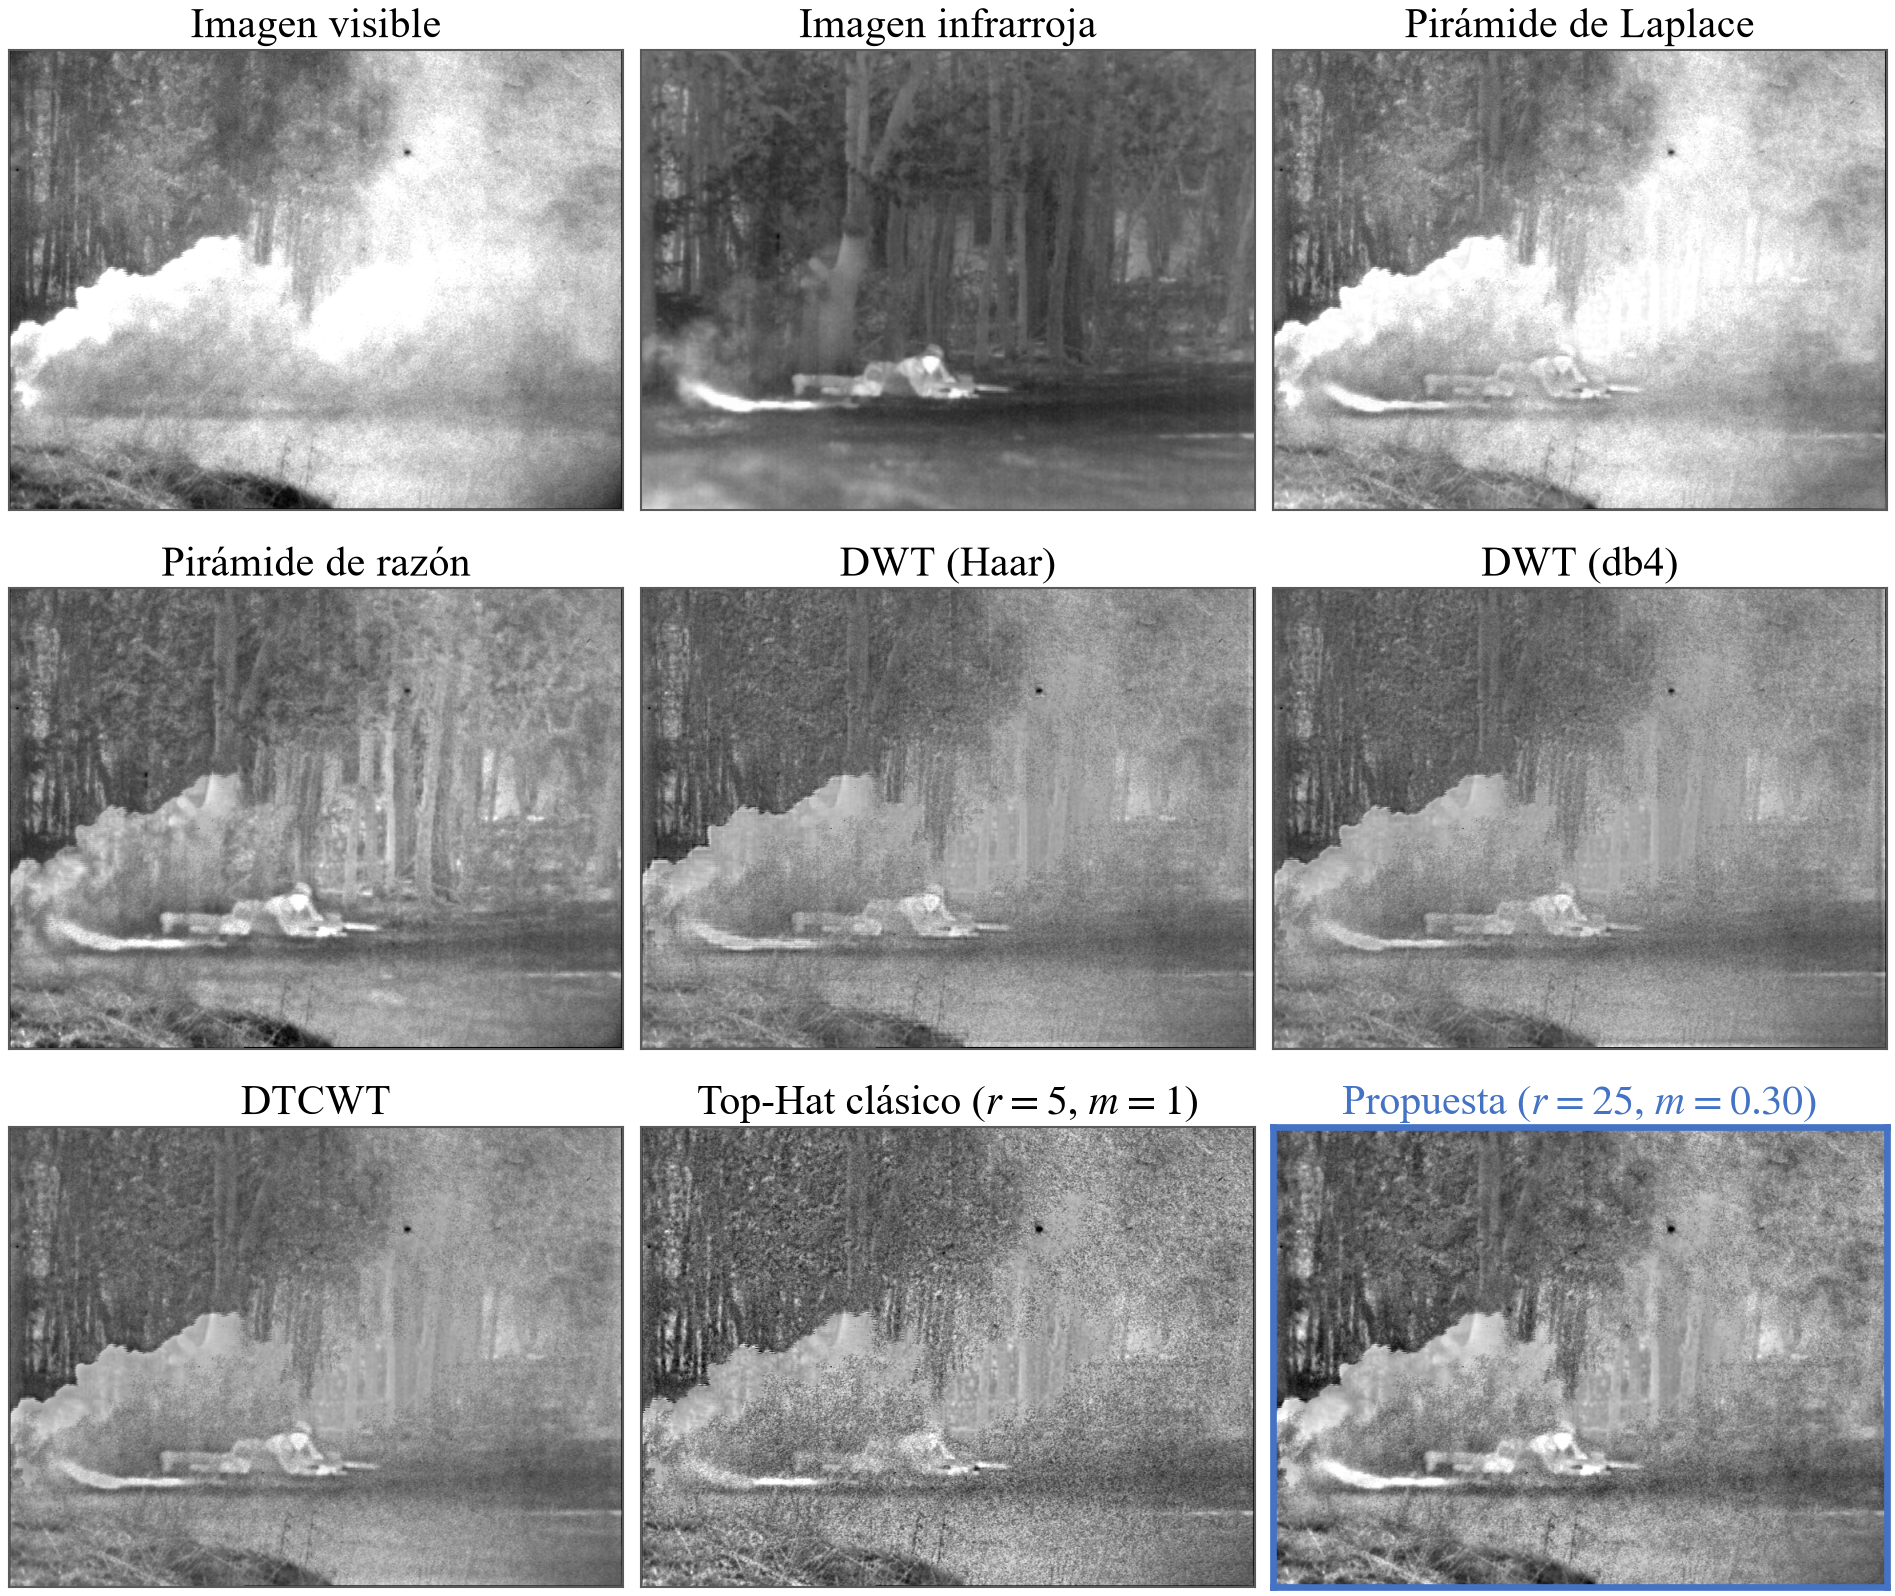
\includegraphics[width=\textwidth]{figuras/montaje_humo}
\nota{Elaboración propia a partir de imágenes del \textit{TNO Image Fusion Dataset} \parencite{toet2014, toet2017}. Es
una de las tres escenas usadas en el ajuste de los parámetros (Sección~\ref{sec:ajuste}). Las dos
primeras imágenes son las fuentes, y las siete siguientes, en orden de lectura, las fusiones de cada
método. La fusión de la propuesta está recuadrada en azul.}
\end{figure}

En la escena del humo, una nube blanca cubre buena parte de la imagen visible y oculta al soldado
tendido detrás de ella. La térmica atraviesa el humo y muestra al soldado junto con los troncos del
bosque. La pirámide de Laplace conservó gran parte del brillo del humo, y en ella el soldado apenas se
insinúa. Las otras seis fusiones atenuaron la cortina y recuperaron la figura del soldado. El Top-Hat
clásico volvió a ser el más granulado. La propuesta, como él, mostró en los árboles y en el pasto más
textura que los cinco métodos multiescala. También dejó algo de grano, aunque menos que el del
Top-Hat clásico.

\section{Resultados cuantitativos}
\label{sec:cuantitativos}

La Tabla~\ref{tab:medias_seis} reúne la media de cada métrica sobre los veinte pares. En las seis, un
valor mayor es mejor. Las tres primeras métricas de la tabla son las de actividad y las tres últimas,
las de fidelidad.

\begin{table}[htbp]
\centering
\caption{Media de las seis métricas por método, sobre los veinte pares del corpus}
\label{tab:medias_seis}
\begin{tabular}{lcccccc}
\toprule
\textbf{Método} & \textbf{EN} & \textbf{SD} & \textbf{MG} & \textbf{MI} & \textbf{SSIM} & \textbf{PSNR} \\
\midrule
Propuesta & \textbf{6.9855} & 0.1439 & 0.0355 & 0.7486 & 0.6584 & 16.84 \\
DTCWT & 6.6877 & 0.1172 & 0.0255 & 0.8755 & \textbf{0.7249} & 17.60 \\
Pirámide de Laplace & 6.8400 & \textbf{0.1550} & 0.0252 & \textbf{1.4210} & 0.7059 & 14.94 \\
Pirámide de razón & 6.8098 & 0.1271 & 0.0275 & 0.7995 & 0.7051 & 17.37 \\
DWT (db4) & 6.6445 & 0.1132 & 0.0260 & 0.8828 & 0.7162 & \textbf{17.65} \\
Top-Hat clásico & 6.9220 & 0.1352 & \textbf{0.0478} & 0.6398 & 0.5640 & 16.87 \\
DWT (Haar) & 6.6816 & 0.1166 & 0.0275 & 0.8711 & 0.7014 & 17.59 \\
\bottomrule
\end{tabular}
\nota{Elaboración propia. En las seis métricas, un valor mayor es mejor, y la negrita marca el mejor valor de cada columna. Los métodos siguen el orden del rango promedio (Tabla~\ref{tab:ranking_seis}). EN: entropía. SD: desviación estándar. MG: gradiente medio. MI: información mutua. SSIM: similitud estructural. En MI y en SSIM, el valor es el promedio del calculado contra la imagen visible y del calculado contra la infrarroja. PSNR: relación señal-ruido de pico, en decibelios, calculada con el promedio de los dos errores cuadráticos medios. DWT (Haar) y DWT (db4) son la misma transformada con dos bases distintas (Sección~\ref{sec:comparativos}). Propuesta: el algoritmo de fusión presentado en este trabajo.}
\end{table}


En las métricas de actividad, la propuesta quedó siempre primera o segunda. Obtuvo la mayor entropía de
los siete métodos, 6.9855, seguida por el Top-Hat clásico, con 6.9220. En desviación estándar quedó
segunda, con 0.1439, detrás de la pirámide de Laplace, que llegó a 0.1550. También fue segunda en gradiente medio, con 0.0355, esta vez detrás del
Top-Hat clásico, con 0.0478. En entropía y en gradiente medio, los dos métodos morfológicos ocuparon los
dos primeros puestos, por delante de los cinco multiescala.

En fidelidad, el orden cambió: la propuesta quedó sexta de siete en cada métrica. Obtuvo 0.7486
en información mutua, 0.6584 en similitud estructural y 16.84 decibelios en relación señal-ruido de
pico. Cada una de esas métricas tuvo un método distinto en el primer puesto. En información mutua fue
la pirámide de Laplace, con 1.4210; en similitud estructural, la DTCWT, con 0.7249, y en relación
señal-ruido de pico, la DWT (db4), con 17.65 decibelios. Solo un método quedó por debajo de
la propuesta: el Top-Hat clásico en las dos primeras y la pirámide de Laplace en la tercera.

La Figura~\ref{fig:metricas_cajas} muestra los veinte valores de cada método en cada métrica, y no solo
su media. La variación de un par a otro es grande frente a la distancia entre las medias. En relación
señal-ruido de pico, por ejemplo, la propuesta va de 11.12 a 21.65 decibelios según el par, mientras
que las medias de los siete métodos quedan entre 14.94 y 17.65. Por eso las cajas se superponen en buena
parte, aunque algunas se separan del resto. En gradiente medio, las de la propuesta y del Top-Hat clásico
quedan enteras a la derecha de las de los cinco métodos multiescala. En información mutua, la de la
pirámide de Laplace queda a la derecha de todas las demás.

\begin{figure}[htbp]
\centering
\caption{Valores de las seis métricas en los veinte pares, por método}
\label{fig:metricas_cajas}
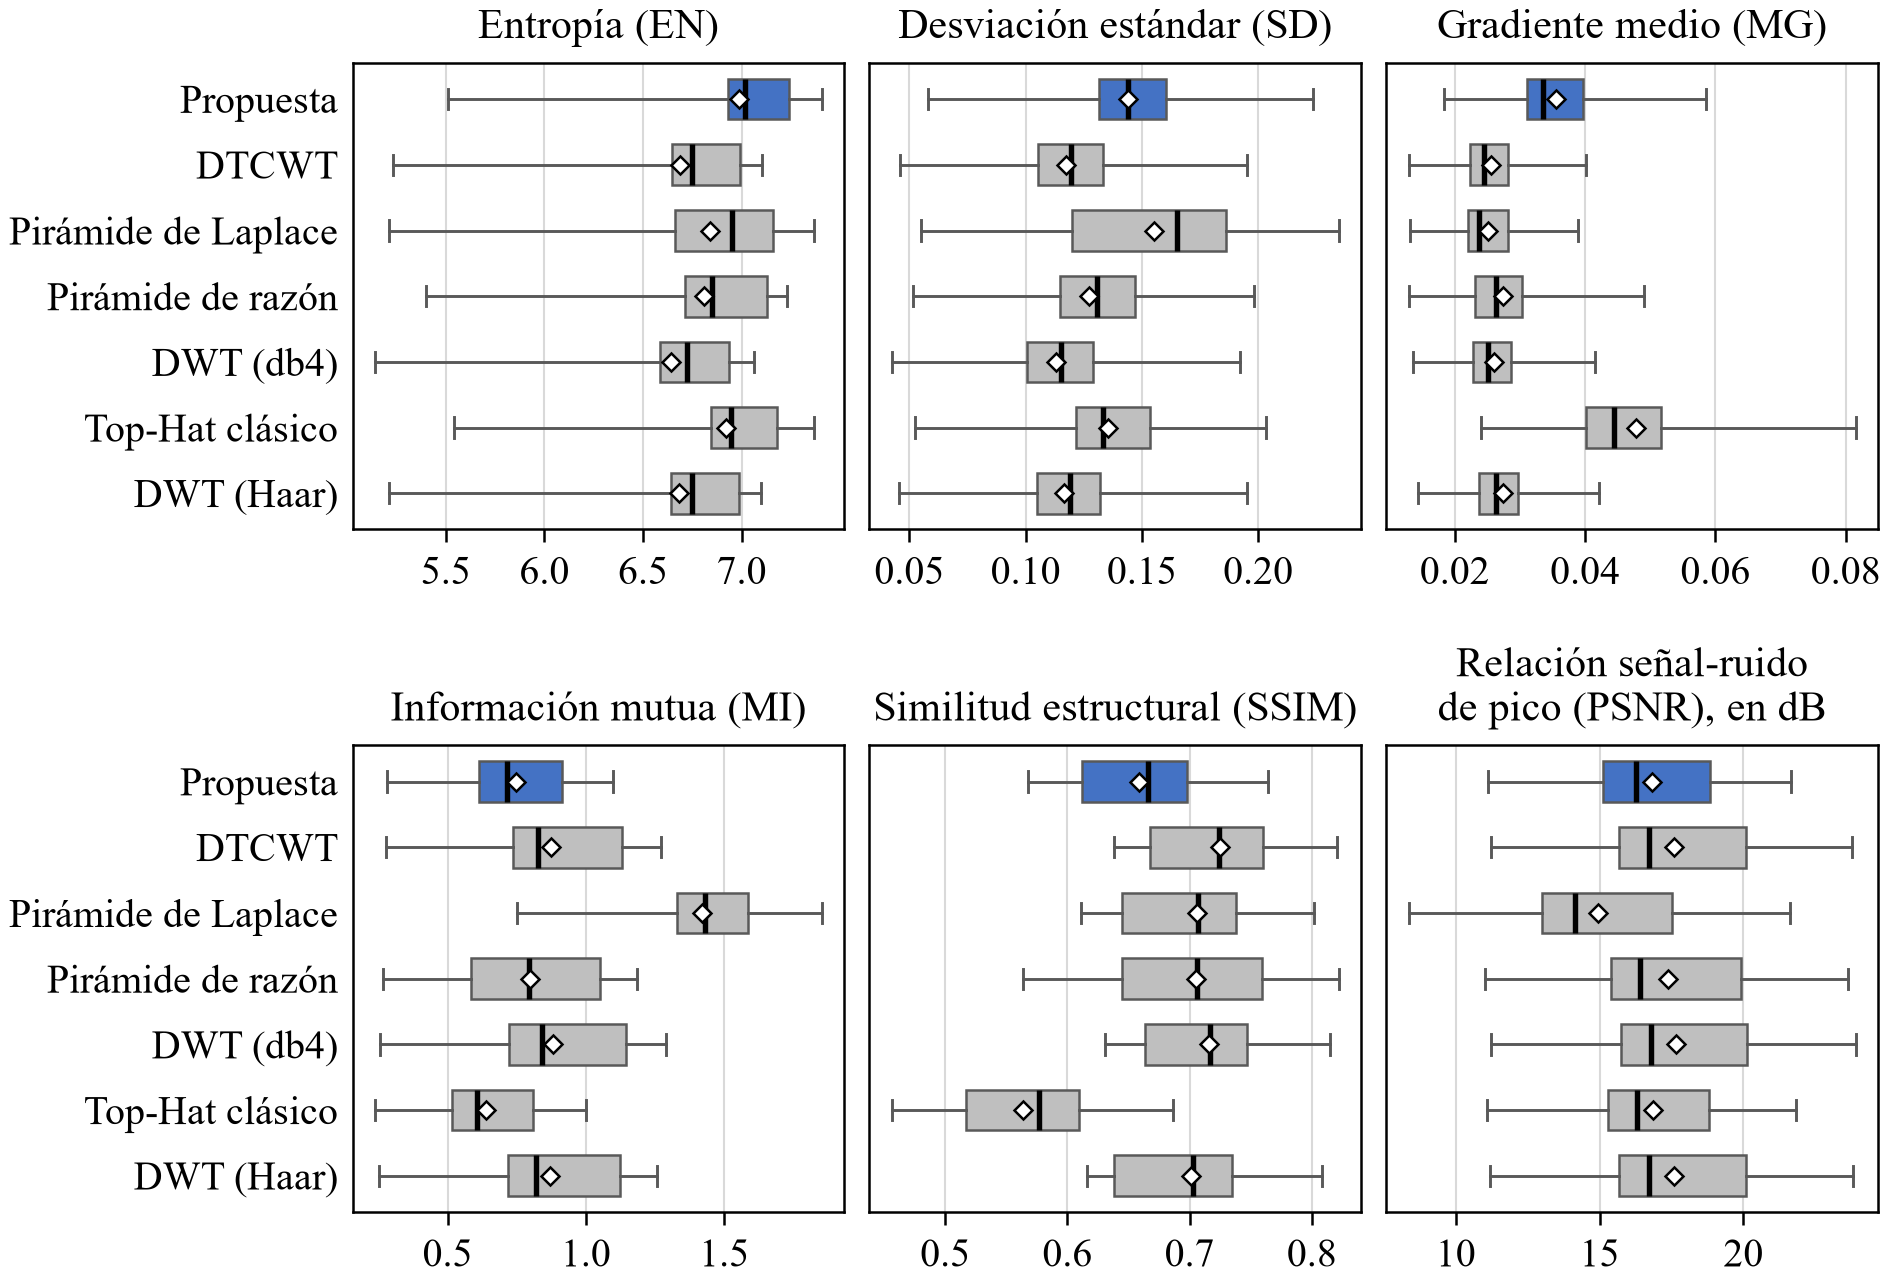
\includegraphics[width=\textwidth]{figuras/fig_metricas_cajas}
\nota{Elaboración propia. Cada caja reúne los veinte valores de un método en una métrica, uno por par
del corpus. La caja abarca la mitad central de esos valores, del primer al tercer cuartil, y la línea
negra es la mediana. El rombo blanco es la media de la Tabla~\ref{tab:medias_seis}, y los bigotes
llegan al mínimo y al máximo. Arriba están las tres métricas de actividad y abajo, las tres de
fidelidad. Los métodos siguen el orden del rango promedio (Tabla~\ref{tab:ranking_seis}), y la propuesta
está en azul.}
\end{figure}

\section{Análisis estadístico}
\label{sec:estadistico}

Ni las medias ni las cajas indican si las diferencias se repiten par a par. Para eso se siguió el
análisis de la Sección~\ref{sec:protocolo-calidad}: la prueba de Friedman por métrica, la clasificación
por rango promedio, los contrastes de Wilcoxon y varias comprobaciones de la solidez del orden.

\subsection{Prueba de Friedman y rango promedio}
\label{sec:res-friedman}

La prueba de Friedman, con los veinte pares como bloques y seis grados de libertad, encontró diferencias
entre los siete métodos en las seis métricas (Tabla~\ref{tab:friedman_seis}). El valor de $p$ fue menor
que 0.001 en todas. El estadístico varió entre 88.3, en entropía, y 111.8, en relación señal-ruido de
pico.

\begin{table}[htbp]
\centering
\caption{Prueba de Friedman por métrica, con siete métodos y veinte pares}
\label{tab:friedman_seis}
\begin{tabular}{lccc}
\toprule
\textbf{Métrica} & \textbf{\boldmath $\chi^2$} & \textbf{\boldmath $p$} & \textbf{¿Difieren?} \\
\midrule
EN & 88.3 & $< 0.001$ & sí \\
SD & 105.1 & $< 0.001$ & sí \\
MG & 101.7 & $< 0.001$ & sí \\
MI & 91.2 & $< 0.001$ & sí \\
SSIM & 100.5 & $< 0.001$ & sí \\
PSNR & 111.8 & $< 0.001$ & sí \\
\bottomrule
\end{tabular}
\nota{Elaboración propia. La prueba contrasta si los rangos promedio de los métodos difieren más de lo esperable por azar. Con siete métodos, tiene seis grados de libertad. La columna ¿Difieren? indica si la diferencia fue significativa, como ocurrió en las seis métricas. En ese caso, algunos métodos quedan mejor o peor ubicados de forma sistemática, par tras par.}
\end{table}


La Tabla~\ref{tab:ranking_seis} y la Figura~\ref{fig:ranking_seis} muestran el rango promedio de cada
método. Es el puesto medio que ocupa sobre los pares y las métricas, de modo que un valor menor es
mejor. La propuesta encabezó la clasificación con 3.642, seguida por la DTCWT, con 3.783, y por la
pirámide de Laplace, con 3.908. Su ventaja sobre la DTCWT fue de 0.14 puestos y no se sometió a una prueba propia. El Top-Hat
clásico quedó sexto de siete, con 4.242.

\begin{table}[htbp]
\centering
\caption{Rango promedio de cada método, por métrica y global}
\label{tab:ranking_seis}
\begin{tabular}{clccccccc}
\toprule
\textbf{Puesto} & \textbf{Método} & \textbf{EN} & \textbf{SD} & \textbf{MG} & \textbf{MI} & \textbf{SSIM} & \textbf{PSNR} & \textbf{Global} \\
\midrule
1 & Propuesta & 1.50 & 1.65 & 2.00 & 5.45 & 5.90 & 5.35 & \textbf{3.642} \\
2 & DTCWT & 4.90 & 5.05 & 6.05 & 3.15 & 1.30 & 2.25 & 3.783 \\
3 & Pirámide de Laplace & 3.25 & 2.00 & 6.25 & 1.20 & 3.80 & 6.95 & 3.908 \\
4 & Pirámide de razón & 3.55 & 3.60 & 4.65 & 4.95 & 3.00 & 4.35 & 4.017 \\
5 & DWT (db4) & 6.85 & 7.00 & 4.75 & 2.65 & 2.50 & 1.00 & 4.125 \\
6 & Top-Hat clásico & 2.45 & 2.85 & 1.00 & 6.80 & 7.00 & 5.35 & 4.242 \\
7 & DWT (Haar) & 5.50 & 5.85 & 3.30 & 3.80 & 4.50 & 2.75 & 4.283 \\
\bottomrule
\end{tabular}
\nota{Elaboración propia. En cada par y en cada métrica, el rango 1 corresponde al mejor método. Cada columna de métrica promedia esos rangos sobre los pares, y la columna Global promedia las seis columnas de métrica. Un valor menor es mejor, y la negrita marca el mejor rango global. La prueba de Friedman opera sobre estos mismos rangos. Propuesta: el algoritmo de fusión presentado en este trabajo.}
\end{table}


\begin{figure}[htbp]
\centering
\caption{Rango promedio de cada método sobre las seis métricas}
\label{fig:ranking_seis}
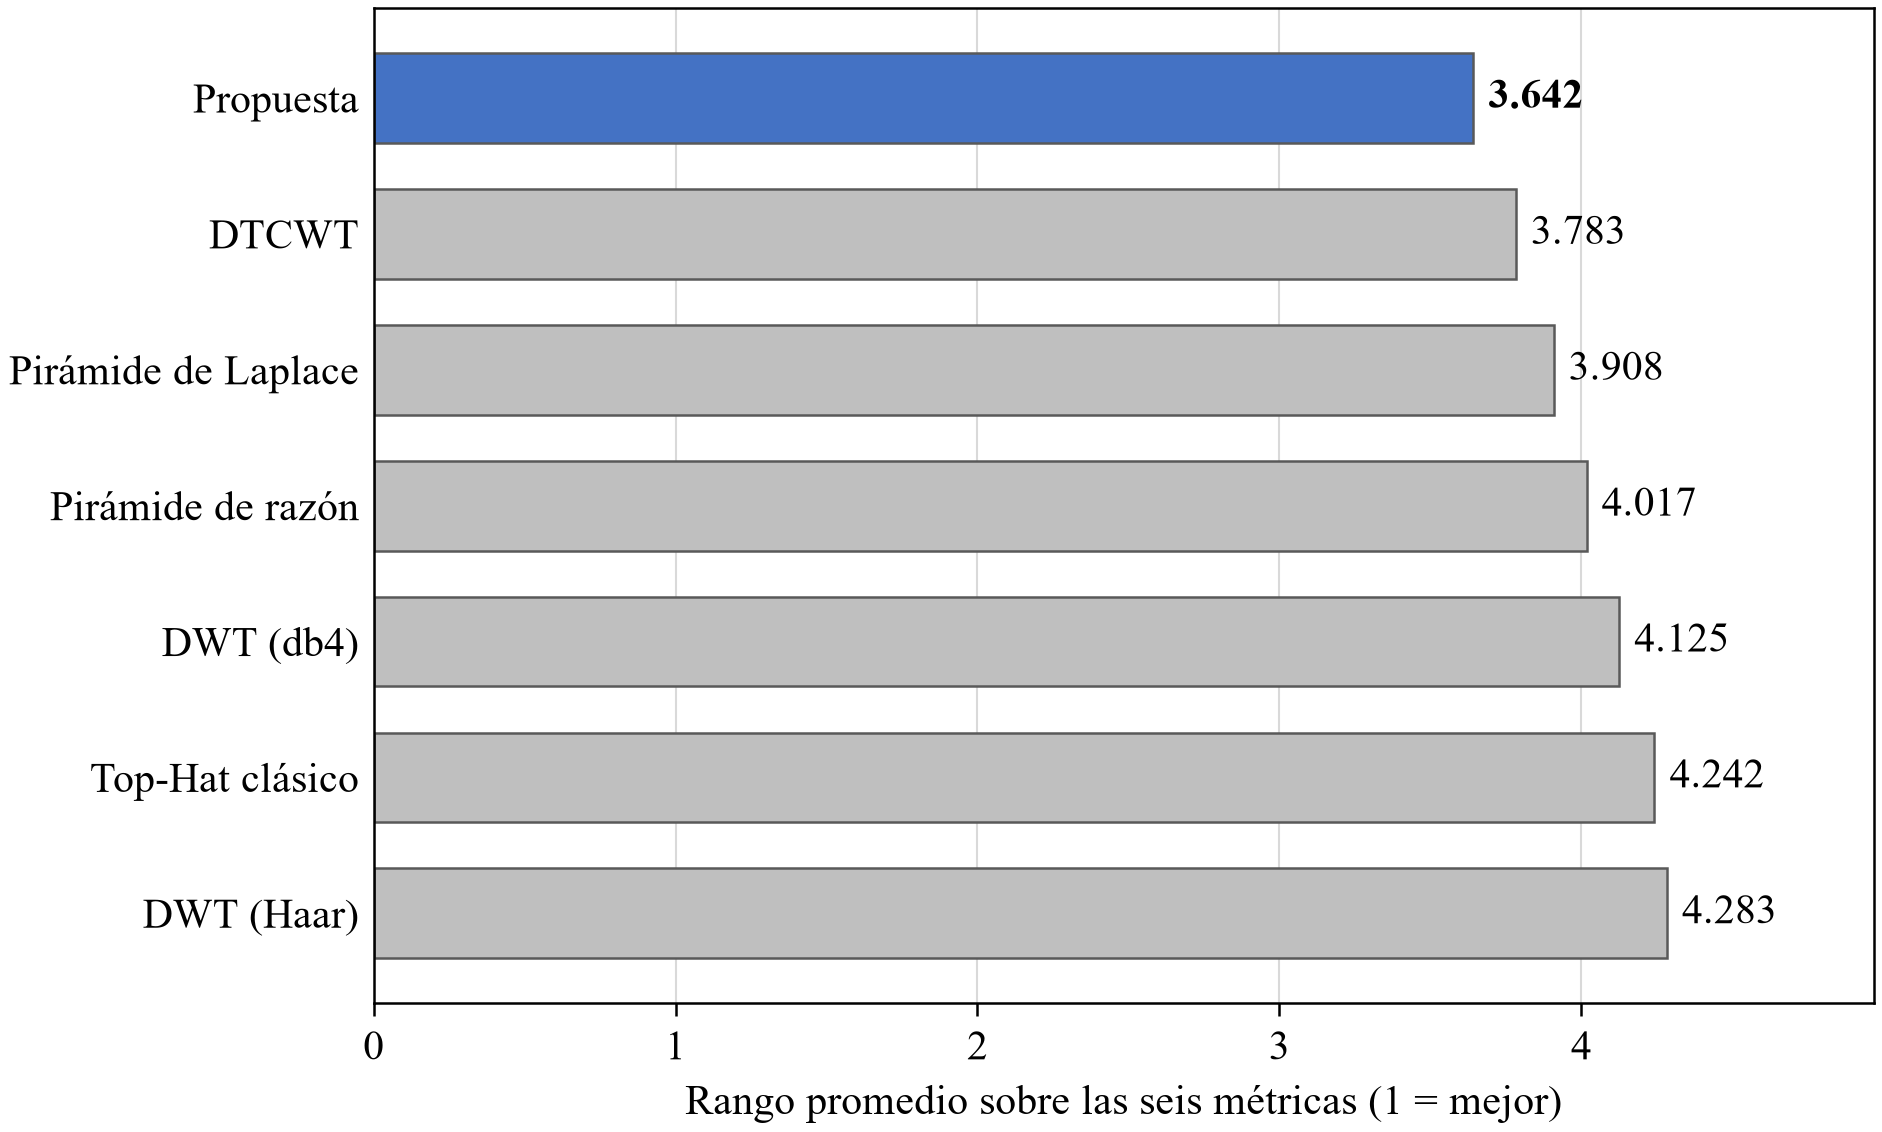
\includegraphics[width=\textwidth]{figuras/fig_ranking_seis}
\nota{Elaboración propia. Cada barra es el puesto medio del método sobre los pares y las métricas, y un
valor menor indica un método mejor ubicado. La propuesta está en azul.}
\end{figure}

Calculado por separado en cada grupo de métricas, el rango promedio muestra perfiles distintos. En las
tres de actividad, la propuesta tuvo 1.717, el mejor de los siete, y en las tres de fidelidad, 5.567, el sexto.
La DTCWT tuvo el perfil opuesto: 5.333 en actividad, sexta, y 2.233 en fidelidad, segunda. La suma de
los dos rangos fue de 7.28 en la propuesta y de 7.57 en la DTCWT. El Top-Hat clásico, sexto en la
clasificación global, obtuvo 2.100 en actividad y 6.383 en fidelidad.

\subsection{Contrastes de Wilcoxon}
\label{sec:res-wilcoxon}

Como la prueba de Friedman resultó significativa en las seis métricas, en cada una se aplicaron los
once contrastes de Wilcoxon, que comparan dos métodos sobre los mismos pares de imágenes. Son sesenta y
seis en total, y sus valores de $p$ se corrigieron con el procedimiento de Holm dentro de cada métrica. La
Tabla~\ref{tab:wilcoxon_resumen} resume los que comparan a la propuesta con los demás métodos. Los once
de cada métrica, incluidos los del Top-Hat clásico frente a los cinco multiescala, figuran en los Anexos
(Tabla~\ref{tab:wilcoxon_completa}).

\begin{table}[htbp]
\centering
\caption{Contrastes de Wilcoxon pareados de la propuesta frente a los demás métodos}
\label{tab:wilcoxon_resumen}
\setlength{\tabcolsep}{5pt}
\begin{tabular}{lccclcc}
\toprule
& \multicolumn{3}{c}{\textbf{Contra los cinco multiescala}} & \multicolumn{3}{c}{\textbf{Contra el Top-Hat clásico}} \\
\cmidrule(lr){2-4}\cmidrule(lr){5-7}
\textbf{Métrica} & \textbf{Gana} & \textbf{Pierde} & \textbf{Empata} & \textbf{Resultado} & \textbf{Diferencia} & \textbf{\boldmath $p$ corregido} \\
\midrule
EN & 5 & 0 & 0 & gana & 0.0636 & $< 0.001$ \\
SD & 4 & 0 & 1 & gana & 0.0087 & $< 0.001$ \\
MG & 5 & 0 & 0 & pierde & $-$0.0123 & $< 0.001$ \\
MI & 0 & 4 & 1 & gana & 0.1089 & $< 0.001$ \\
SSIM & 0 & 5 & 0 & gana & 0.0944 & $< 0.001$ \\
PSNR & 1 & 4 & 0 & empata & $-$0.0319 & 0.674 \\
\bottomrule
\end{tabular}
\nota{Elaboración propia. Gana, Pierde y Empata cuentan los contrastes de la propuesta con los cinco métodos multiescala. Resultado, Diferencia y $p$ corregido se refieren a su contraste con el Top-Hat clásico. Un contraste significativo al 5~\% después de corregir por comparaciones múltiples, con Holm sobre los once contrastes de cada métrica, cuenta como victoria o derrota de la propuesta según el signo de la diferencia de medias. Uno no significativo cuenta como empate. Diferencia: media de la propuesta menos media del Top-Hat clásico, en las unidades de cada métrica (decibelios en PSNR). El Top-Hat clásico se usó con radio 5 y peso 1.}
\end{table}


Frente a los cinco métodos multiescala, la propuesta ganó casi todos los contrastes de actividad y
perdió casi todos los de fidelidad. Ganó los cinco de entropía y los cinco de gradiente medio, y en
desviación estándar ganó cuatro y empató con la pirámide de Laplace. En fidelidad perdió los cinco
contrastes de similitud estructural. En información mutua perdió cuatro y empató con la pirámide de
razón, y en relación señal-ruido de pico perdió cuatro y le ganó a la pirámide de Laplace.

Frente al Top-Hat clásico, la propuesta ganó en cuatro métricas, perdió en una y empató en otra. Las
cuatro victorias tuvieron un $p$ corregido menor que 0.001, con diferencias de medias de 0.0636 en
entropía, 0.0087 en desviación estándar, 0.1089 en información mutua y 0.0944 en similitud
estructural. La derrota fue en gradiente medio, con una diferencia de $-0.0123$ y un $p$ corregido también menor que 0.001. En relación señal-ruido de pico, la
diferencia de $-0.0319$ decibelios no fue significativa: su $p$ corregido fue de 0.674, de modo que esa
métrica cuenta como empate.

\subsection{Solidez del orden}
\label{sec:res-robustez}

Al repetir el análisis con trece bloques, uno por escena, la cabeza de la clasificación no cambió: la
propuesta siguió primera, con 3.590, y la DTCWT, segunda, con 3.756. La prueba de Friedman volvió a
ser significativa en las seis métricas, con $p$ menor que 0.001 y estadísticos entre 56.6 y 73.0. Los sesenta y seis contrastes de
Wilcoxon conservaron su signo, y sesenta y cinco conservaron además su decisión. El único que cambió fue
el del Top-Hat clásico frente a la pirámide de razón en desviación estándar. Su $p$ corregido pasó de
0.005 con veinte pares a 0.098 con trece bloques, y el contraste dejó de ser significativo.

El puesto de la propuesta, en cambio, dependió del conjunto de métricas. Con las nueve métricas
iniciales quedó primera, con 3.394, seguida por la pirámide de Laplace, con 3.911. Con las diecisiete
que se calcularon quedó tercera, con 3.459, detrás de la pirámide de Laplace, con 3.147, y de la DTCWT,
con 3.259. Las ocho métricas que se suman a las nueve iniciales, entre ellas Qabf, Nabf, SCD, VIF y
FMI, comparan la fusión con sus fuentes, de modo que doce de las diecisiete son de ese tipo. Las tres
clasificaciones usan la misma escala, de 1 a 7, pero promedian métricas distintas; por eso se compara
el puesto y no el valor.

En el control con imágenes degradadas, que mide si el ruido recibe premio, se ordenaron catorce entradas
con las seis métricas, en una escala de 1 a 14. Las entradas fueron los siete métodos, el promedio simple y seis
imágenes degradadas a partir de ese promedio. El promedio con ruido ganó puestos a medida que crecía el
ruido. Con una desviación estándar del ruido de 0.02 quedó decimotercero; con 0.05, duodécimo, y con
0.10, décimo. Con 0.20 empató en el octavo puesto con el Top-Hat clásico, ambos con 7.483, y fue la mejor de las catorce entradas en las tres métricas de
actividad. El Top-Hat clásico quedó así como el último de los siete métodos en ese control.

La cabeza del control la ocuparon la pirámide de Laplace, con 6.633, y el promedio simple, con 6.650.
La propuesta quedó tercera, con 6.725. Ese puesto depende de las entradas que se ordenan. Con
solo los siete métodos y el promedio simple, en una escala de 1 a 8, la propuesta queda primera, con
4.142, y el promedio, sexto, con 4.633. El cambio lo producen las dos versiones desenfocadas, que en
puesto medio quedan delante de la propuesta en las tres métricas de fidelidad y detrás del promedio
simple en las seis.

\section{Aplicación a la detección de objetos}
\label{sec:deteccion}

Los treinta detectores previstos, tres por cada una de las diez entradas, completaron su entrenamiento.
Esta sección presenta primero los objetos de una sola cámara y las tasas de acierto de cada entrada.
Después compara la propuesta con el Top-Hat clásico, y al final reúne las medidas secundarias y el
seguimiento del entrenamiento.

\subsection{Objetos de una sola cámara y tasas de acierto}
\label{sec:res-tasas}

Los cuadros de seguimiento sirvieron para calibrar el umbral principal. En ellos, con el umbral de 0.25,
los detectores de la visible cometieron en promedio 0.948 falsos positivos de personas y luces por
imagen. Los umbrales con que cada detector más se acercó a ese valor, que forman el umbral principal de la
Sección~\ref{sec:det-medida}, quedaron entre 0.24 y 0.27.

Con el umbral principal, los detectores de la visible y de la infrarroja definieron 211 objetos vistos
solo por la visible y 622 vistos solo por la infrarroja. Otros 724 los encontraron los detectores de
las dos cámaras. Con el umbral fijo de 0.25, esos tres conjuntos tuvieron 209, 624 y 728 objetos, y con
el de mejor equilibrio por clase, 197, 633 y 667. Los objetos de una sola cámara quedaron repartidos en
diez de los once grupos de la prueba. El reparto fue muy desigual: de los 211 objetos de solo la
visible, 176 provienen de dos grupos, con 86 y 90. El de 90, el mayor de la prueba, reúne también 219
de los 622 de solo la infrarroja.

La Figura~\ref{fig:m3fd_ejemplo} muestra un cuadro nocturno de la prueba con dos objetos de una sola
cámara, uno de cada cámara. El semáforo encendido, que M3FD marca como luz, solo lo encuentran los
detectores de la imagen visible, y la persona del borde izquierdo, solo los de la infrarroja. Con la
primera semilla, es decir, en el primer entrenamiento de cada entrada, el detector del Top-Hat clásico
encontró el semáforo y el de la propuesta no. Ninguno de los dos encontró a la persona del borde, y
los dos encontraron a la que está delante del auto y a otra lejana. Como se trata de un solo
cuadro y una sola semilla, el ejemplo no representa el resultado de conjunto.

\begin{figure}[htbp]
\centering
\caption{Detecciones del Top-Hat clásico y de la propuesta en un cuadro nocturno de M3FD}
\label{fig:m3fd_ejemplo}
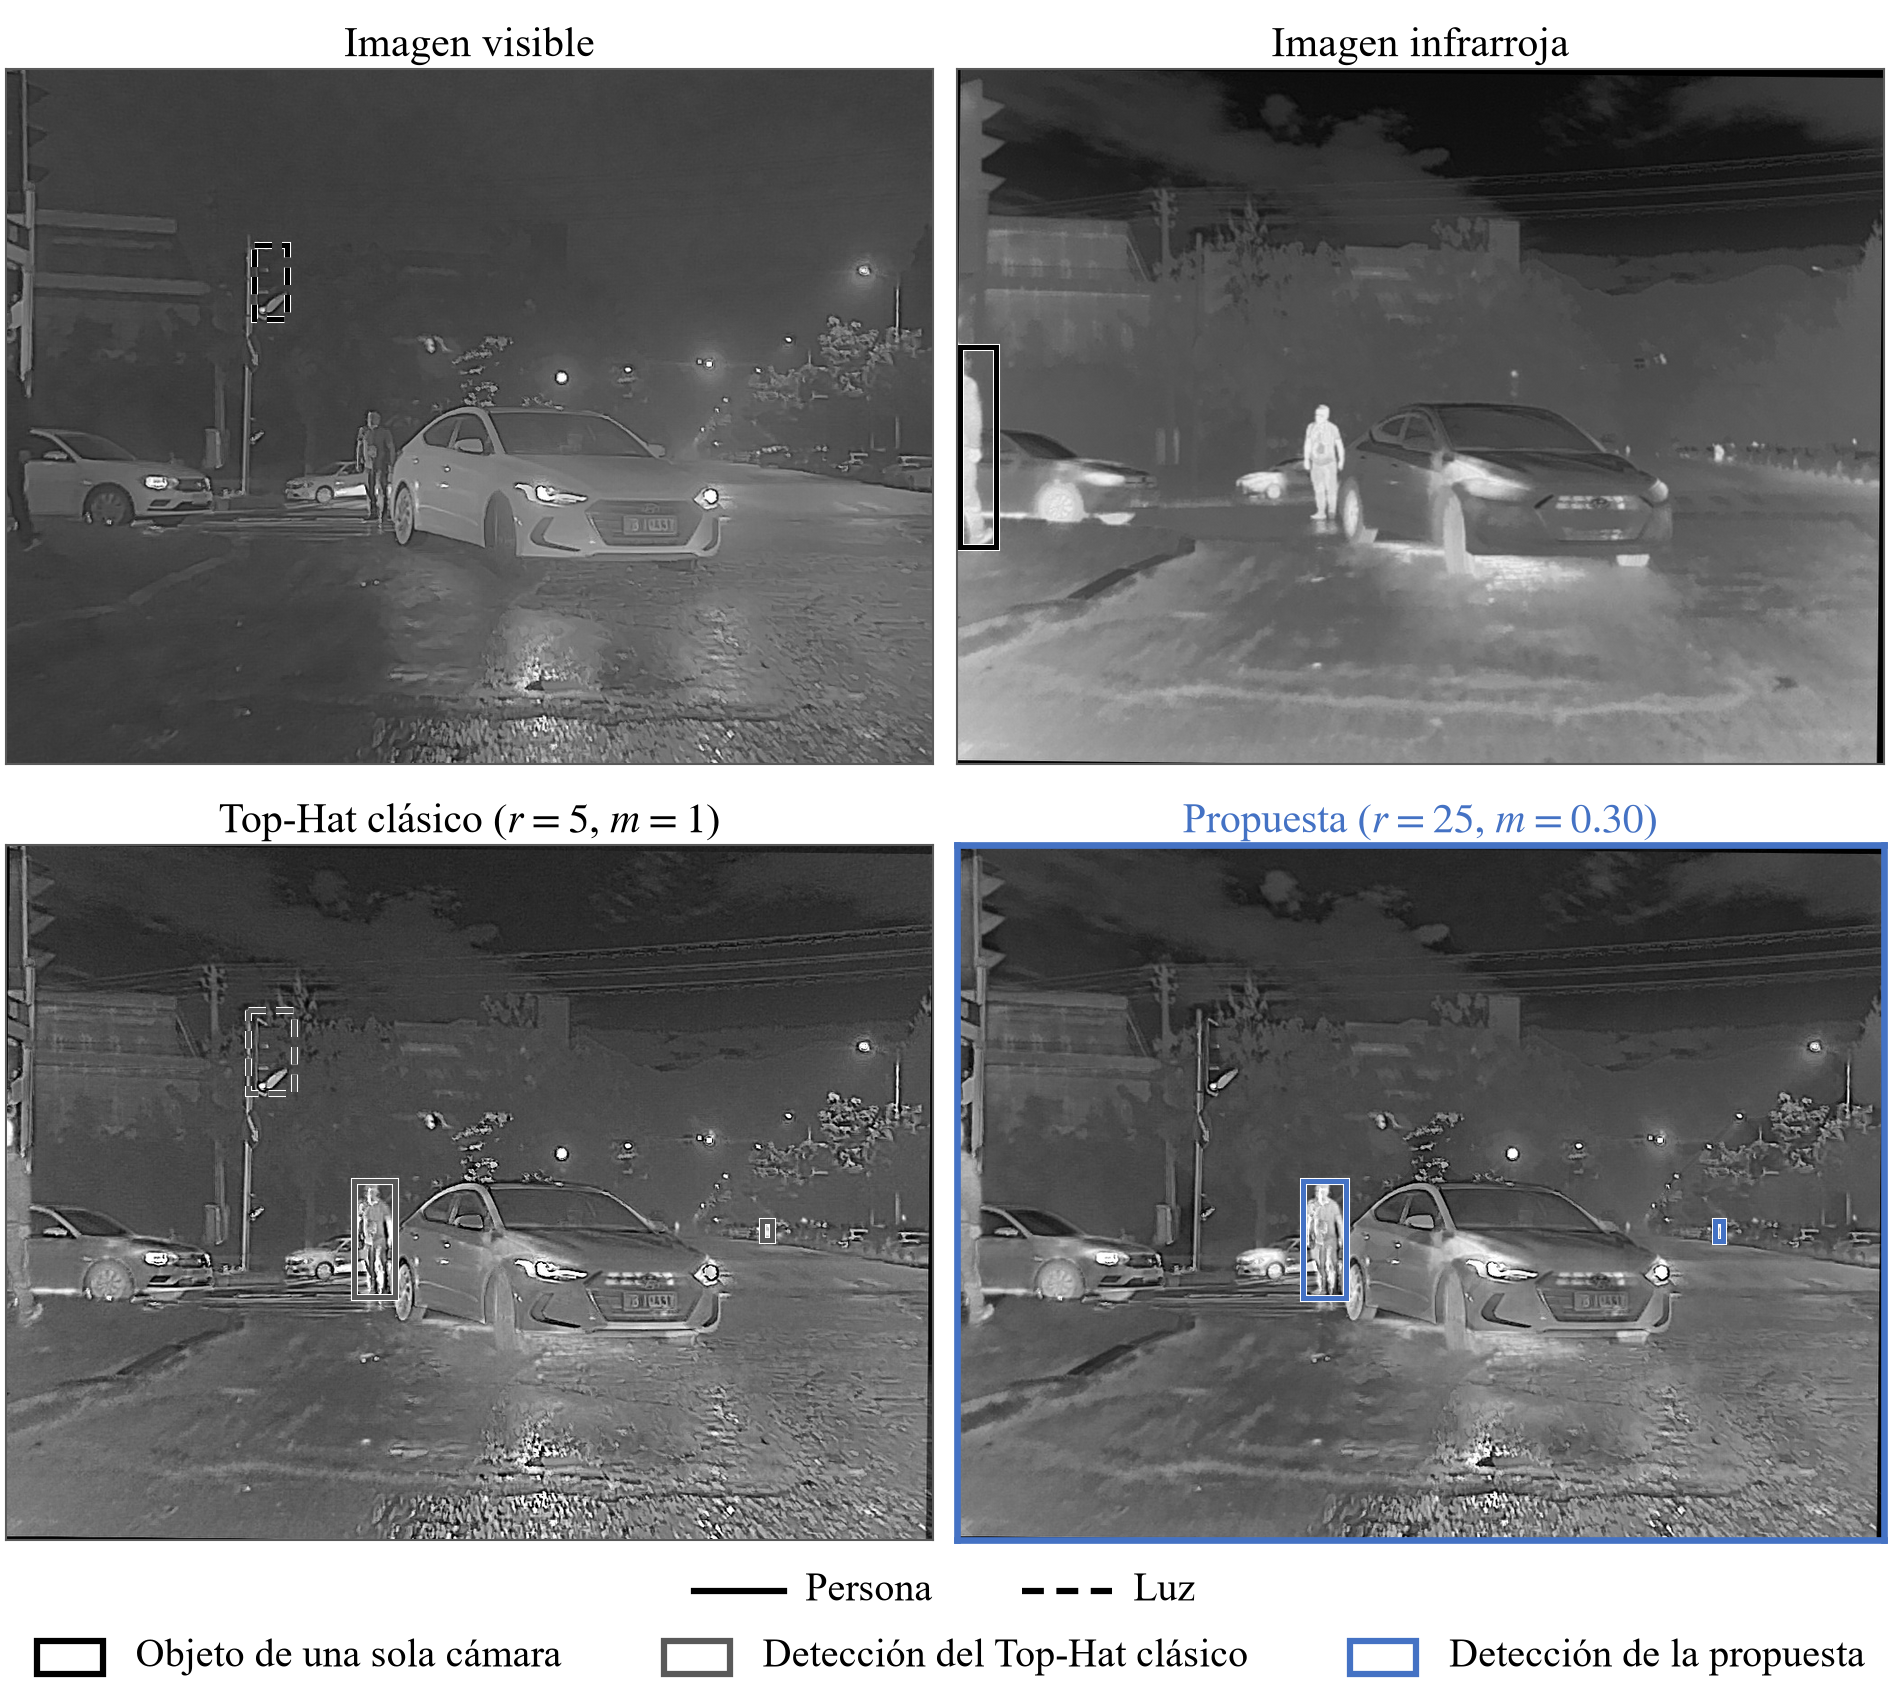
\includegraphics[width=\textwidth]{figuras/fig_m3fd_ejemplo}
\nota{Elaboración propia a partir de imágenes de M3FD \parencite{liu2022}. Es el cuadro 437 del
conjunto y pertenece a la prueba. Se eligió sin mirar las detecciones de las fusiones. De los 49
cuadros con al menos un objeto de solo la visible y uno de solo la infrarroja, 12 tienen marcadas en
M3FD las dos clases del análisis, personas y luces. Entre esos 12, es el que tiene los objetos de una sola cámara más grandes. Arriba están
las fuentes en escala de grises, tal como las recibe el detector. En cada una, el recuadro negro
marca su objeto de una sola cámara. Abajo, cada fusión lleva las detecciones de su detector, con la primera
semilla y su umbral principal: 0.26 en el Top-Hat clásico y 0.25 en la propuesta. La línea continua
marca personas, y la discontinua, luces.}
\end{figure}

La Tabla~\ref{tab:v2_tasas} presenta la tasa de acierto de las ocho entradas fusionadas. Están ordenadas
por tasa equilibrada, que promedia la tasa sobre los objetos de solo la visible y la tasa sobre los de
solo la infrarroja. La visible y la infrarroja no figuran en ella, porque sus detectores son los que
definen los objetos de una sola cámara.

\begin{table}[htbp]
\centering
\caption{Tasa de acierto de las entradas fusionadas en la detección de objetos}
\label{tab:v2_tasas}
\begin{tabular}{lcccc}
\toprule
\textbf{Entrada} & \textbf{Solo visible} & \textbf{Solo infrarroja} & \textbf{Equilibrada} & \textbf{De ambas} \\
\midrule
Pirámide de Laplace & 60.5 & 72.5 & \textbf{66.5} & 97.1 \\
DTCWT & 53.7 & 72.2 & 62.9 & 94.1 \\
DWT (Haar) & 53.7 & 70.9 & 62.3 & 95.9 \\
Propuesta & 55.6 & 67.2 & 61.4 & 94.4 \\
DWT (db4) & 51.2 & 69.2 & 60.2 & 96.0 \\
Promedio simple & 49.1 & 71.3 & 60.2 & 95.1 \\
Top-Hat clásico & 51.3 & 65.5 & 58.4 & 94.1 \\
Pirámide de razón & 49.0 & 57.3 & 53.1 & 93.0 \\
\bottomrule
\end{tabular}
\nota{Elaboración propia. Las tasas están en porcentaje y se calcularon con el umbral principal. El umbral principal de cada detector se fijó para que este cometiera, en los cuadros de seguimiento, tantos falsos positivos de personas y luces por imagen como los detectores de la visible con un umbral de 0.25. Solo visible y Solo infrarroja se calculan sobre los objetos que ve una sola cámara: 211 vistos solo por la visible y 622 solo por la infrarroja. La columna De ambas se calcula sobre los 724 objetos que ven las dos cámaras. La columna Equilibrada es el promedio de las dos columnas anteriores. Las filas van de mayor a menor tasa equilibrada, y la mayor está en negrita. Cada tasa promedia, sobre tres semillas, la fracción de objetos encontrados. La visible y la infrarroja no figuran porque sus detectores definen qué objetos ve una sola cámara. Propuesta: el algoritmo de fusión presentado en este trabajo.}
\end{table}


La pirámide de Laplace obtuvo la mayor tasa equilibrada, 66.5~\%. La propuesta quedó cuarta de ocho,
con 61.4~\%, y el Top-Hat clásico, séptimo, con 58.4~\%. El Top-Hat clásico quedó así por debajo del
promedio simple, que obtuvo 60.2~\%, aunque esa diferencia no se sometió a prueba.

Al separar las dos tasas que forman la equilibrada, la propuesta fue segunda en los objetos vistos solo
por la visible, con 55.6~\%, detrás de la pirámide de Laplace. En los vistos solo por la infrarroja fue
sexta, con 67.2~\%. Sobre los objetos que veían las dos cámaras, todas las entradas alcanzaron al menos
el 93.0~\%. Con el umbral fijo de 0.25, la propuesta obtuvo una tasa equilibrada de 61.1~\% y quedó
cuarta; con el de mejor equilibrio por clase, obtuvo 59.0~\% y quedó quinta.

La Figura~\ref{fig:m3fd_aciertos} muestra dos escenas de la prueba con un objeto de una sola cámara,
uno de cada cámara, que el detector de la propuesta encontró. Arriba, en un cuadro nocturno, la
persona de la derecha apenas se distingue del fondo en la imagen visible y se ve nítida en la
infrarroja. Con la primera semilla, el detector de la visible no la encontró, y sí los de la
infrarroja, del Top-Hat clásico y de la propuesta. Abajo, en un cuadro diurno, la imagen visible
muestra encendidas las flechas de los dos semáforos y el número del de la derecha; en la infrarroja,
los dos son manchas claras sin esos detalles. Con la primera semilla, los detectores de la visible, del
Top-Hat clásico y de la propuesta encontraron el semáforo de la derecha, y el de la infrarroja no. En
toda la prueba, las dos fusiones coincidieron en la mayoría de estos objetos: con esa misma semilla, de
los que encontró al menos una de ellas, las dos encontraron 83 de 143 de solo la visible y 355 de 460
de solo la infrarroja. Como la Figura~\ref{fig:m3fd_ejemplo}, esta
ilustra cómo una fusión puede encontrar un objeto que una de las cámaras pierde, y no el resultado de
conjunto, que es el de la Tabla~\ref{tab:v2_tasas}.

\begin{figure}[htbp]
\centering
\caption{Detecciones en dos cuadros de M3FD con un objeto de una sola cámara}
\label{fig:m3fd_aciertos}
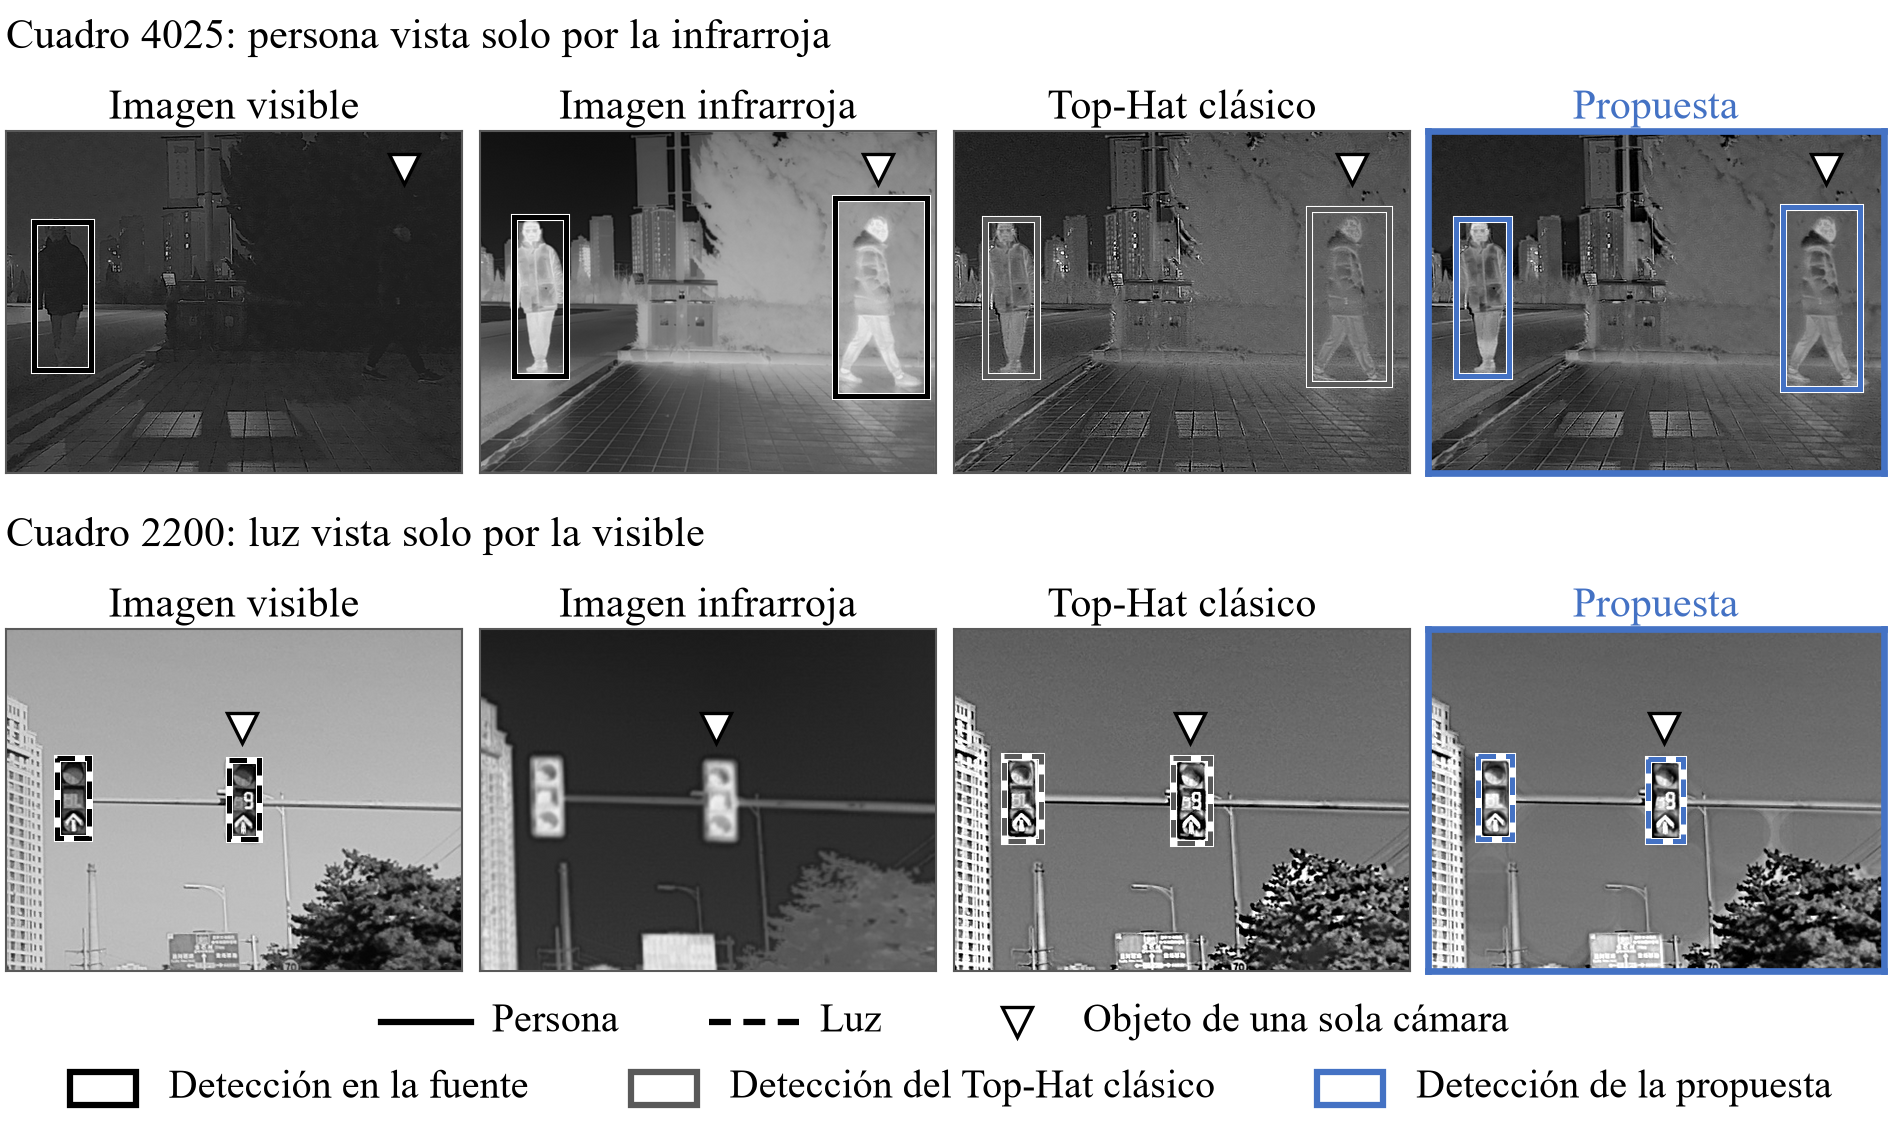
\includegraphics[width=\textwidth]{figuras/fig_m3fd_aciertos}
\nota{Elaboración propia a partir de imágenes de M3FD \parencite{liu2022}. Son los cuadros 4025 y 2200
del conjunto y pertenecen a la prueba. Se eligieron con una regla fija que no usa las detecciones del
Top-Hat clásico. Entre los objetos de una sola cámara que encontró el detector de la propuesta con la
primera semilla, fuera del grupo del cuadro 437 de la Figura~\ref{fig:m3fd_ejemplo}, arriba está el de
solo la infrarroja de mayor área según su marca en M3FD, y abajo, el de solo la visible de mayor área
entre los de otro grupo que el de arriba. Como la regla parte de los objetos que encontró la
propuesta, la figura no indica con qué frecuencia los encuentra. Arriba se muestra el cuadro entero,
y abajo, un recorte de $475 \times 356$ píxeles alrededor del objeto, el mismo en los cuatro paneles.
Cada panel lleva las detecciones de su detector con la primera semilla y el umbral principal: 0.25 en
la visible y en la propuesta, y 0.26 en la infrarroja y en el Top-Hat clásico. Los objetos de una sola
cámara se definen con los tres detectores de cada cámara, y los paneles muestran solo el primero. Por
eso, abajo, el de la infrarroja tampoco encuentra el semáforo de la izquierda, que es de las dos
cámaras porque lo encontraron los otros dos detectores de la infrarroja. El triángulo
señala el objeto de una sola cámara. A diferencia de la Figura~\ref{fig:m3fd_ejemplo}, los recuadros
negros no son objetos marcados, sino detecciones en las fuentes; los gris oscuro, del Top-Hat clásico
($r = 5$, $m = 1$), y los azules, de la propuesta ($r = 25$, $m = 0.30$). La línea continua marca
personas, y la discontinua, luces.}
\end{figure}

\subsection{Comparación con el Top-Hat clásico}
\label{sec:res-tophat}

La Tabla~\ref{tab:deteccion_tophat} reúne la diferencia de tasa equilibrada entre la propuesta y el
Top-Hat clásico, con su intervalo de confianza del 95~\%, para cada umbral y para el \textit{bootstrap}
salvaje por grupos.

\begin{table}[htbp]
\centering
\caption{Diferencia de tasa equilibrada entre la propuesta y el Top-Hat clásico}
\label{tab:deteccion_tophat}
\begin{tabular}{lcc}
\toprule
\textbf{Cálculo} & \textbf{Diferencia} & \textbf{Intervalo del 95~\%} \\
\midrule
Umbral principal & 3.0 & [0.0, 6.0] \\
Umbral fijo de 0.25 & 2.7 & [0.0, 5.3] \\
Umbral de mejor equilibrio por clase & 2.5 & [1.1, 3.9] \\
\addlinespace \textit{Bootstrap} salvaje por grupos & 3.0 & [$-$3.5, 5.5] \\
\bottomrule
\end{tabular}
\nota{Elaboración propia. La diferencia, en puntos porcentuales, es la tasa de acierto equilibrada de la propuesta menos la del Top-Hat clásico. El cálculo de los intervalos de confianza del 95~\% se describe en la Sección~\ref{sec:det-comparacion}. La unidad del análisis es el grupo de bloques contiguos de cuadros: de los once grupos de la prueba, entran los diez que tienen objetos de una sola cámara. Las tres primeras filas usan un error estándar robusto por grupos y la distribución $t$ con nueve grados de libertad \parencite{cameron2015}. La última fila usa el umbral principal y un \textit{bootstrap} salvaje por grupos, estudentizado y con la hipótesis nula impuesta \parencite{cameron2008, webb2023}. Su intervalo reúne las diferencias que esa prueba no rechaza al 5~\%, y el valor $p$ para una diferencia nula es 0.17. Los límites inferiores que se muestran como 0.0 son positivos: 0.02 puntos con el umbral principal y 0.05 con el umbral fijo. Según el par de semillas, la diferencia va de $-$3.1 a 7.8 puntos con el umbral principal. Con el umbral fijo va de $-$2.9 a 7.1, y con el de mejor equilibrio por clase, de $-$5.2 a 9.1. Con cada umbral, tres de las nueve diferencias son negativas: frente a una misma semilla del Top-Hat clásico, las tres semillas de la propuesta quedan por debajo. Por eso la diferencia no es robusta a la semilla.}
\end{table}


Con el umbral principal, la propuesta aventajó al Top-Hat clásico, pero el intervalo de confianza apenas
dejó fuera el cero. Su tasa equilibrada fue 3.0 puntos porcentuales mayor, con un intervalo de 0.0 a
6.0. El límite inferior exacto fue de 0.02 puntos, que con un decimal se muestra
como 0.0. La diferencia, además, no es robusta a la semilla: según el par de semillas, va de $-3.1$ a
7.8 puntos.

Con el umbral fijo de 0.25, la diferencia fue de 2.7 puntos, con un intervalo de 0.0 a 5.3 y un límite
inferior exacto de 0.05. Con el umbral de mejor equilibrio por clase fue de 2.5 puntos, con un intervalo
de 1.1 a 3.9. Los tres intervalos calculados con la distribución $t$ dejaron fuera el cero, los dos
primeros por muy poco. El \textit{bootstrap} salvaje por grupos, estudentizado y con la hipótesis nula
impuesta, no lo excluyó. Con el umbral principal dio un valor de $p$ de 0.17 y un intervalo de $-$3.5 a
5.5, y con los otros dos umbrales, valores de $p$ de 0.17 y 0.08. Al dejar fuera el grupo mayor de la
prueba, la diferencia con el umbral principal bajó de 3.0 a 1.5 puntos; al dejar fuera cualquiera de
los otros, quedó entre 2.3 y 3.6.

La Figura~\ref{fig:deteccion_tasas} muestra la tasa equilibrada de cada semilla en las ocho entradas
fusionadas y las nueve diferencias entre las semillas de la propuesta y las del Top-Hat clásico. Las
tres semillas de la propuesta quedaron a menos de un punto entre sí, mientras que las del Top-Hat
clásico se separaron casi diez. Por eso las diferencias entre pares de semillas no mantuvieron el signo.
Con el umbral principal, seis fueron positivas y tres negativas, de $-2.2$, $-3.1$ y $-2.3$ puntos. Las
tres negativas se dieron frente a la misma semilla del Top-Hat clásico, la de tasa más alta, que superó
a las tres de la propuesta. Con los otros dos umbrales hubo también tres diferencias negativas, otra vez
frente a esa semilla. Según el par de semillas, la diferencia fue de $-2.9$ a 7.1 puntos con el umbral
fijo de 0.25 y de $-5.2$ a 9.1 con el de mejor equilibrio por clase.

Como referencia, con el mismo cálculo, la diferencia entre la propuesta y el promedio simple fue de 1.2
puntos, con un intervalo de $-6.6$ a 9.0, que incluye valores de los dos signos. Frente a la pirámide de
Laplace, la propuesta quedó por debajo en los nueve pares de semillas, con diferencias de $-5.8$ a
$-4.6$ puntos.

\begin{figure}[htbp]
\centering
\caption{Tasa equilibrada por entrada y diferencia entre la propuesta y el Top-Hat clásico}
\label{fig:deteccion_tasas}
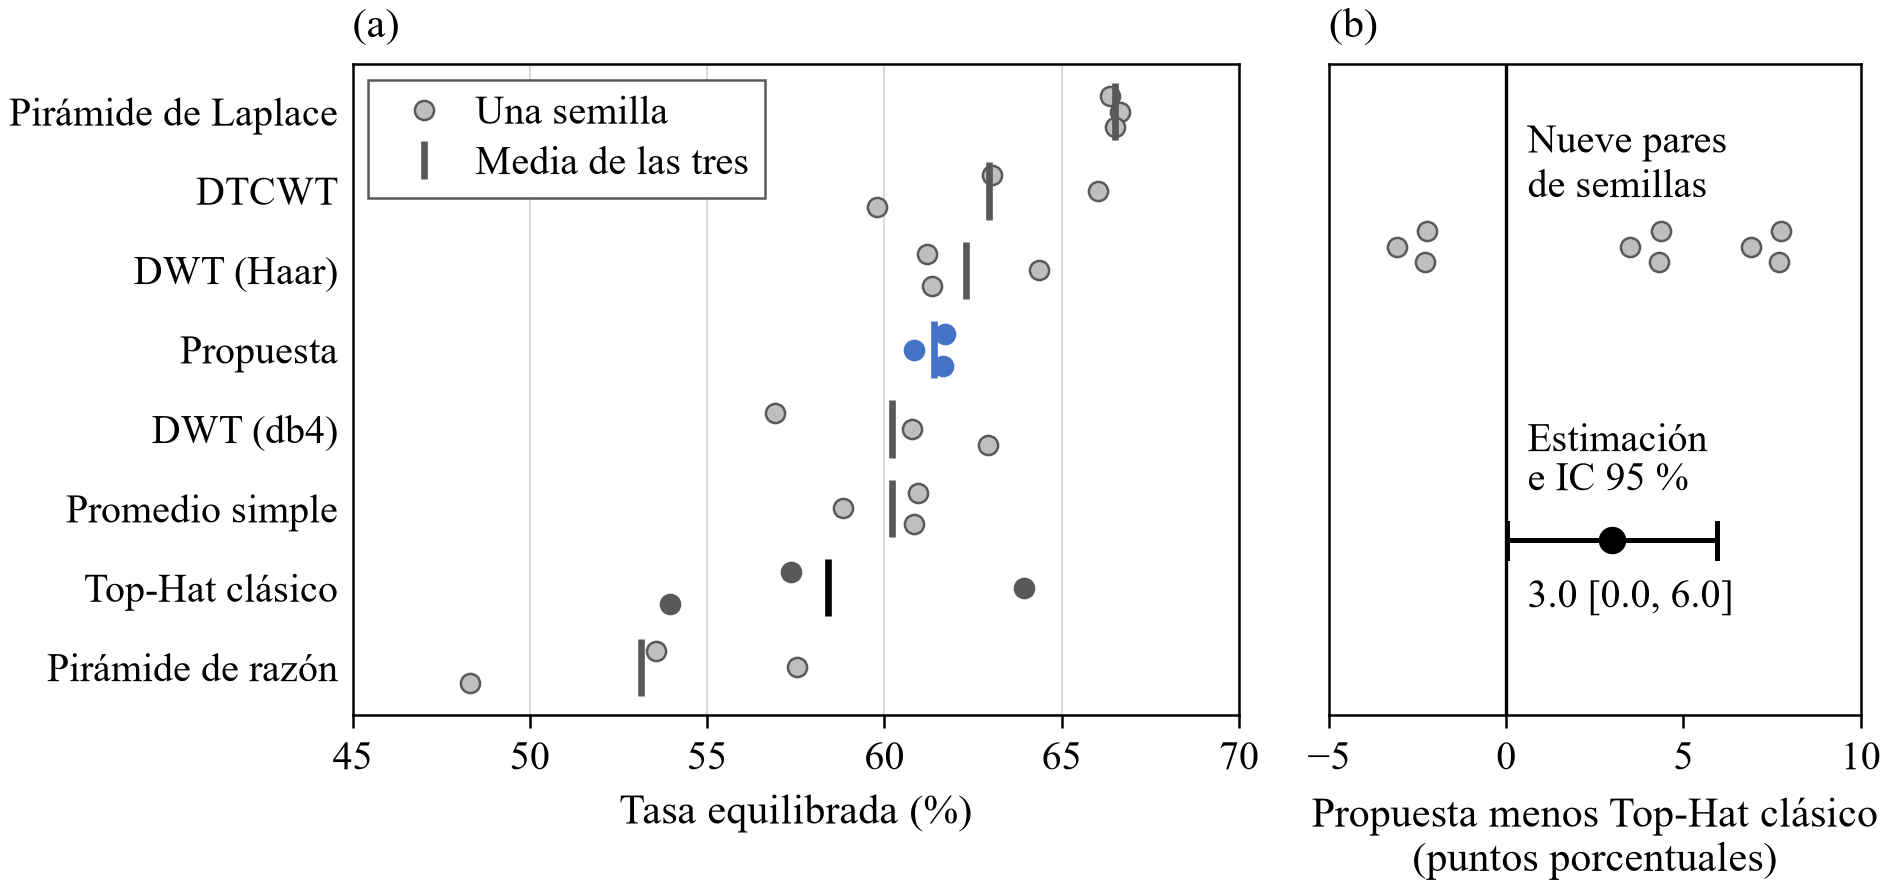
\includegraphics[width=\textwidth]{figuras/fig_deteccion_tasas}
\nota{Elaboración propia. Las tasas corresponden al umbral principal. (a) Las ocho entradas fusionadas
de la Tabla~\ref{tab:v2_tasas}, ordenadas de mayor a menor tasa. Cada punto es la tasa de una semilla del detector,
y la línea vertical, la media de las tres semillas, que es el valor de la tabla. La propuesta está en azul y el Top-Hat
clásico, en gris oscuro, con su media en negro. (b) Diferencia de tasa equilibrada, propuesta menos
Top-Hat clásico, en puntos porcentuales. Arriba están las nueve diferencias entre cada semilla de la propuesta y cada semilla del
Top-Hat clásico. Abajo están la estimación principal y su intervalo, con los límites entre corchetes. A
la derecha del cero, la propuesta acierta más que el Top-Hat clásico. Los dos paneles tienen la misma
escala horizontal: un punto porcentual mide lo mismo en ambos. IC 95~\%: intervalo de confianza del
95~\%.}
\end{figure}

La ventaja de la propuesta frente al Top-Hat clásico es, entonces, mínima y depende de la semilla, por
lo que queda como un hallazgo por confirmar.

\subsection{Medidas secundarias y entrenamiento}
\label{sec:res-secundarias}

La mAP50, la precisión media global sobre las seis clases, se midió en los 1197 cuadros que dejó el
primer filtro (Sección~\ref{sec:det-datos}). En esta medida, la propuesta quedó séptima de diez, por
debajo del Top-Hat clásico. La pirámide de Laplace obtuvo el mayor valor, 0.441, muy cerca de la DTCWT,
con 0.440, y del promedio simple, con 0.439. Siguieron el Top-Hat clásico, con 0.434, la DWT (db4), con
0.430, la infrarroja sola, con 0.429, y la propuesta, con 0.427. Cerraron la lista la DWT (Haar), con
0.415, la pirámide de razón, con 0.411, y la visible sola, con 0.363.

Así, cinco de las ocho entradas fusionadas superaron en mAP50 a la infrarroja sola. La propuesta no
estuvo entre ellas: quedó apenas por debajo, con 0.427 frente a 0.429, una diferencia menor que la
variación entre sus propias semillas, que fue de 0.419 a 0.440.

En los 49 cuadros con al menos un objeto de solo la visible y uno de solo la infrarroja, los detectores
de la propuesta encontraron al menos uno de cada tipo en el 57.1~\% de los casos. Con el Top-Hat
clásico la proporción fue algo mayor, 57.8~\%, y con la pirámide de Laplace llegó al 72.1~\%. Sobre los
objetos vistos por las dos cámaras, la propuesta y el Top-Hat clásico quedaron casi iguales, con 94.4~\% y 94.1~\%.
Ninguna de estas diferencias, ni las de mAP50, se sometió a prueba.

El seguimiento época por época se hizo solo con la primera semilla de cada entrada, midiendo la mAP50
sobre los 474 cuadros de seguimiento. Esos cuadros provienen de los mismos bloques que el
entrenamiento. En la época 40, su mAP50 fue de 0.73 a 0.76, muy superior a la de esos mismos detectores en los
1197 cuadros, de 0.35 a 0.46. Por eso, ese seguimiento refleja más el ajuste a cuadros parecidos a los de entrenamiento que la
capacidad de generalizar. Al final del entrenamiento, esa medida seguía subiendo en
casi todos los detectores: en las últimas cinco épocas, nueve de los diez tenían todavía una pendiente
positiva. La excepción fue el de la DWT (Haar). Entre las épocas 30 y 40 cambió, además, el orden de la propuesta
frente a dos métodos. En la época 30 quedaba por debajo de la pirámide de Laplace y de la DWT (db4), y
en la 40, por encima de ambas. En ese tramo, la propuesta pasó de 0.7347 a 0.7636; la pirámide de
Laplace, de 0.7406 a 0.7616, y la DWT (db4), de 0.7372 a 0.7512.

Por último, se calculó la correlación de Spearman entre el rango promedio de calidad, con 1 para el
mejor, y la tasa equilibrada de los siete métodos. Resultó de $\rho = -0.32$, con $p = 0.48$. El signo
negativo indica que los métodos mejor ubicados en calidad detectaron algo más, pero la correlación no
fue significativa. Los dos órdenes, además, provienen de conjuntos distintos: el de calidad, del TNO, y
el de detección, de M3FD.

\section{Examen de la hipótesis}
\label{sec:res-hipotesis}

Esta sección reúne, para cada afirmación de la hipótesis (Capítulo~\ref{cap:introduccion}), los
resultados con que se la examina según la Sección~\ref{sec:examen-hipotesis}. No se hizo ninguna prueba
nueva: todos los valores provienen de las secciones anteriores.

La primera afirmación compara la calidad de la propuesta con la del Top-Hat clásico. En los seis
contrastes de Wilcoxon con la corrección de Holm, la propuesta ganó en entropía, desviación estándar,
información mutua y similitud estructural (Tabla~\ref{tab:wilcoxon_resumen}). Perdió en gradiente medio
y empató en relación señal-ruido de pico, donde el $p$ corregido fue de 0.674. Como complemento, el rango
promedio fue de 3.642 en la propuesta, primera de siete, y de 4.242 en el Top-Hat clásico, sexto.

La segunda afirmación se refiere a los cinco métodos multiescala. Con las seis métricas, la propuesta
encabezó la clasificación por rango promedio: obtuvo 3.642, frente a 3.783 de la DTCWT. El margen, de
0.14 puestos, no tiene una prueba propia. Con las nueve métricas iniciales también quedó primera, y con
las diecisiete, tercera. Su perfil fue desigual entre los dos grupos de métricas. Ganó los cinco contrastes
de entropía y de gradiente medio, y cuatro de cinco en desviación estándar. Perdió los cinco de
similitud estructural y cuatro de cinco en información mutua y en relación señal-ruido de pico. Por
grupos de métricas, su rango promedio fue el mejor de los siete en actividad, 1.717, y el sexto en
fidelidad, 5.567.

La tercera afirmación corresponde a la aplicación. Con el umbral principal, la tasa equilibrada de la
propuesta superó a la del Top-Hat clásico en 3.0 puntos, con un intervalo de 0.0 a 6.0 y un límite
inferior exacto de 0.02. Esa diferencia no es robusta a la semilla: entre los nueve pares de semillas
fue de $-3.1$ a 7.8 puntos, y cada uno de los tres umbrales dejó tres diferencias negativas. Con los
otros dos umbrales, el límite inferior del intervalo también quedó por encima de cero. El
\textit{bootstrap} salvaje por grupos, en cambio, no excluyó el cero: con el umbral principal, su valor
de $p$ fue de 0.17.

Con esos resultados, la parte de la hipótesis que trata de la calidad se sostiene en lo principal. La
propuesta superó al Top-Hat clásico en cuatro de las seis métricas, y su calidad fue comparable a la de los cinco
métodos multiescala. Su primer puesto por rango promedio se apoya en un margen estrecho, sin una prueba
propia, y cambia con el conjunto de métricas. En la aplicación, la ventaja frente al Top-Hat clásico es
mínima: el límite inferior del intervalo apenas superó el cero, el \textit{bootstrap} no lo excluyó y
la diferencia no es robusta a la semilla. Esa parte de la hipótesis queda, por eso, como un hallazgo que falta confirmar con más grupos,
más semillas y otros detectores (Capítulo~\ref{cap:recomendaciones}).

\chapter{Discusión}
\label{cap:discusion}

El Capítulo~\ref{cap:introduccion} planteó dos preguntas, y los resultados las responden con distinto grado
de firmeza. La primera se refería a la calidad de las imágenes del algoritmo propuesto. Esas imágenes
fueron mejores que las del Top-Hat clásico en cuatro de las seis métricas. Frente a los cinco métodos
multiescala, la calidad del algoritmo fue comparable, aunque con un perfil propio: más actividad y menos
fidelidad. Sus imágenes tienen más información, contraste y nitidez, pero se parecen menos a las
fuentes. La propuesta encabezó la clasificación por rango promedio, pero por un margen estrecho y sin
que ese margen se sometiera a prueba. La segunda pregunta era si un detector entrenado con esas imágenes
encuentra más objetos vistos por una sola cámara que uno entrenado con las del Top-Hat clásico. El
detector encontró algo más, pero la ventaja es mínima. La tasa equilibrada, que promedia el acierto en
los objetos de solo la visible y de solo la infrarroja, fue 3.0 puntos mayor que la del Top-Hat
clásico, con un intervalo de 0.0 a 6.0. Según el par de semillas, esa diferencia cambia de signo. Así,
en calidad la hipótesis se sostiene en lo principal; en la detección, la ventaja queda como un hallazgo
por confirmar. El capítulo discute esos
resultados en cinco ejes: el perfil de calidad y su costo, el ajuste de los parámetros, la aplicación a
la detección, la relación entre calidad y detección y, al final, las limitaciones del estudio.

\section{La calidad de la fusión y su costo}
\label{sec:disc-calidad}

El primer puesto por rango promedio, con 3.642 frente a 3.783 de la DTCWT (Tabla~\ref{tab:ranking_seis}),
no autoriza a decir que la propuesta supere a ese método. Esa diferencia no tiene una prueba propia, y los
dos métodos llegan a la cabeza por caminos opuestos. La propuesta fue primera en actividad y sexta en
fidelidad; la DTCWT, sexta en actividad y segunda en fidelidad. Como cada grupo reúne tres métricas, el
rango global lo decide la suma de los dos rangos parciales: 7.28 para la propuesta y 7.57 para la DTCWT.
Un perfil marcado no basta, por sí solo, para llegar a la cabeza. La DWT (db4), todavía más
desequilibrada que la DTCWT entre los dos grupos, quedó quinta.

El perfil de la propuesta nace de la regla de fusión (Ecuación~\ref{eq:regla-tophat}), que toma su forma del realce de
contraste de la Ecuación~\eqref{eq:realce} \parencite{bai2012}. Sumar el detalle claro y restar el oscuro
agranda la diferencia de brillo entre cada detalle y su entorno, pero aleja la imagen de sus fuentes. El
barrido del peso lo confirma (Sección~\ref{sec:res-ajuste}). Con la propuesta y con el Top-Hat clásico,
subir $m$ elevó la desviación estándar y el gradiente medio y bajó las tres métricas de fidelidad. El
compromiso es, entonces, propio de la regla y no depende del banco de elementos. Algo parecido observaron
\textcite{bajacfigueredo2024} con otra variable. Al agrandar el elemento estructurante de 3 a 9,
subieron la desviación estándar, la entropía y la frecuencia espacial, y la información mutua bajó o se
mantuvo.

El costo se ve también en las imágenes. La resta del detalle oscuro es el único término de la regla que
lleva un píxel por debajo del promedio de las fuentes, y puede bajarlo hasta el negro, donde el valor se
recorta. De ahí el borde oscuro que rodea a la persona en la Figura~\ref{fig:montaje_kaptein}.

Frente al Top-Hat clásico, la propuesta ganó en entropía, desviación estándar, información mutua y
similitud estructural, perdió en gradiente medio y empató en PSNR (Tabla~\ref{tab:wilcoxon_resumen}). Ese
reparto no puede atribuirse al banco, porque entre los dos métodos cambian a la vez los elementos, el radio
y el peso. Según el barrido, el peso mueve por sí solo tres de esas métricas en la dirección
observada. Con los dos operadores, un peso menor reduce el gradiente medio y eleva la
información mutua y la similitud estructural. La propuesta usa un peso de 0.30, y el Top-Hat clásico,
de 1, así que parte de esas diferencias puede deberse solo a ese peso menor.

El primer puesto depende también del conjunto de métricas. Con las nueve métricas iniciales, cinco de
ellas de actividad, la propuesta quedó primera. Con un conjunto de diecisiete, en el que doce comparan
la fusión con sus fuentes, bajó al tercer puesto, detrás de la pirámide de Laplace y de la DTCWT. Por
otra parte, los cinco métodos multiescala se usaron con sus parámetros por defecto, mientras que el radio
de la propuesta se eligió sobre los mismos veinte pares de la evaluación (Sección~\ref{sec:ajuste}).
Nada asegura que el orden se mantenga si todos se ajustan con un mismo criterio.

El control con imágenes degradadas marca el límite de las métricas de actividad: una ventaja en ellas
no prueba, por sí sola, que el detalle agregado sea útil. Cuanto más ruido se agregó al promedio simple,
más puestos ganó la imagen resultante, hasta empatar en el octavo con el Top-Hat clásico
(Sección~\ref{sec:res-robustez}). Con la mayor intensidad fue, además, la mejor de las catorce entradas
en las tres métricas de actividad. En ese mismo control, la propuesta quedó tercera, detrás de la
pirámide de Laplace y del promedio simple sin degradar. Ese puesto lo producen las dos versiones
desenfocadas, que en fidelidad quedaron delante de la propuesta y, en las seis métricas, detrás del promedio
simple. Al ordenar solo los siete métodos y el promedio, la propuesta quedó primera, y el promedio, sexto. La cabeza de la clasificación resistió también el análisis por
escenas. Con un bloque por escena,
la propuesta siguió primera y la DTCWT segunda, y solo uno de los sesenta y seis contrastes cambió su
decisión.

\section{El ajuste de los parámetros}
\label{sec:disc-ajuste}

Las veinticinco corridas del enjambre terminaron con el peso en 0.30, el límite inferior del rango de
búsqueda. La grilla de comprobación indica que ese valor es un borde y no un máximo interior. En cada
radio, el mejor peso quedó muy por debajo de ese límite. A partir de 0.30, la aptitud, la función que
el enjambre busca maximizar, bajó con cada aumento del peso (Sección~\ref{sec:res-ajuste}). Una
explicación posible está en la forma de la aptitud (Ecuación~\ref{eq:aptitud}). Dos de sus tres términos, la similitud estructural y la PSNR, premian el
parecido con las fuentes, y cada aumento del peso aleja de ellas la fusión. La entropía, el tercer
término, no compensa esa pérdida.

El resultado difiere del de \textcite{ortegarodriguez2025}, que buscaron el peso en el mismo rango.
Hicieron 125 corridas, con veinticinco configuraciones en cada una de cinco escenas, y el peso terminó
en 0.30 solo en 17, todas de una misma escena. Aquel trabajo usó la aptitud original, que aquí se
adaptó, ajustó los parámetros escena por escena y empleó un disco único. Cualquiera de esas diferencias
podría explicar el contraste, que no se investigó. La última tiene una lectura directa. El detalle del
banco puede llegar al doble del de un disco del mismo radio (Ecuación~\ref{eq:banco}), así que un
mismo peso aleja más la fusión de sus fuentes.

En el radio, el enjambre no llegó a un valor único, porque con $m = 0.30$ la aptitud tiene dos máximos
locales: uno en $r = 1$ y otro, menor, en $r = 25$. Casi todas las corridas, incluidas las quinientas de
control, terminaron en uno de esos dos radios (Sección~\ref{sec:res-ajuste}), y la mayor aptitud
corresponde a $r = 1$. Aun así, se adoptó $r = 25$ porque prioriza el realce: con $r = 1$, el disco y
los segmentos miden apenas tres píxeles de ancho y solo extraen detalles muy finos. Frente a $r = 1$, el
radio adoptado fue mejor en todas las métricas de actividad y peor en todas las de fidelidad. Esa
elección explica en parte la ventaja de la propuesta sobre los métodos multiescala en entropía,
desviación estándar y gradiente medio.

\section{La aplicación a la detección}
\label{sec:disc-deteccion}

La ventaja de la propuesta frente al Top-Hat clásico, de 3.0 puntos de tasa equilibrada, admite dos
lecturas (Tabla~\ref{tab:deteccion_tophat}). La primera se apoya en el intervalo de confianza del
95~\%, de 0.0 a 6.0, que excluye el cero por muy poco: su límite inferior es de 0.02 puntos. El cero
queda fuera también con los otros dos umbrales, pero no con el \textit{bootstrap} salvaje por grupos,
más confiable cuando los grupos son pocos y de tamaño desigual. Con el umbral principal, ese cálculo
dio un intervalo de $-3.5$ a 5.5 y un valor de $p$ de 0.17. La segunda lectura surge de los pares de
semillas. Sus nueve diferencias van de $-3.1$ a 7.8 puntos, y las tres
negativas enfrentan a la propuesta con una misma semilla del Top-Hat clásico.

Las dos lecturas no se contradicen. El intervalo mide cómo varía la diferencia entre los grupos de
cuadros. Como la tasa de cada objeto llega ya promediada sobre las tres semillas, el intervalo no recoge
por completo la variación del entrenamiento. Los pares de semillas, en cambio, la dejan a la vista: basta que un
detector del Top-Hat clásico acierte más que los otros dos para invertir el signo en tres de los nueve
pares. Por eso la ventaja es mínima, y queda como un hallazgo por confirmar con más grupos, más semillas
y otros detectores (Capítulo~\ref{cap:recomendaciones}).

El hallazgo, además, no aísla el efecto del banco. Entre la propuesta y el Top-Hat clásico cambian a la vez
los elementos, el radio y el peso (Sección~\ref{sec:operador}), y la comparación no dice cuál de esos
cambios produce la diferencia. Tampoco muestra que el detalle agregado ayude a detectar. El promedio
simple es la regla de la Ecuación~\eqref{eq:regla-tophat} con peso cero, de modo que la comparación con
él mide el aporte del detalle. El Top-Hat clásico tuvo una tasa menor que la de ese promedio
(58.4~\% contra 60.2~\%, sin prueba entre ambos). Como referencia, la propuesta superó a ese promedio
por apenas 1.2 puntos. El intervalo de esa diferencia, calculado del mismo modo que el de la
Tabla~\ref{tab:deteccion_tophat}, va de $-6.6$ a 9.0 e incluye el cero.

Aun si se confirmara, la ventaja frente al Top-Hat clásico no pondría a la propuesta entre las mejores
entradas para detectar. Entre las ocho entradas fusionadas quedó cuarta, con 61.4~\%, y la pirámide de Laplace
tuvo la mayor tasa, 66.5~\% (Tabla~\ref{tab:v2_tasas}). Esa pirámide superó a la propuesta con todas las
combinaciones de semillas. En la mAP50, una medida secundaria calculada sobre todas las clases, cinco de
las ocho entradas fusionadas superaron a la infrarroja sola. La propuesta no estuvo entre ellas, aunque
su diferencia con la infrarroja fue menor que la variación entre sus propias semillas
(Sección~\ref{sec:res-secundarias}). En esa medida y en los cuadros con un objeto de cada cámara,
además, el Top-Hat clásico quedó apenas por encima de la propuesta, sin prueba entre ambos.

Estas comparaciones valen para un entrenamiento de cuarenta épocas. En el seguimiento hecho con la
primera semilla de cada entrada, nueve de los diez detectores todavía mejoraban al final del
entrenamiento su mAP50 sobre los cuadros de seguimiento, que no son los de la prueba. Entre las épocas 30 y 40, además, la propuesta pasó de estar por debajo a estar por encima
de la pirámide de Laplace y de la DWT (db4) en esa medida (Sección~\ref{sec:res-secundarias}). Con un
entrenamiento más largo, el orden entre entradas de tasa parecida podría cambiar.

\section{Relación entre calidad y detección}
\label{sec:disc-relacion}

Los dos planos de la evaluación no ordenaron a los métodos de la misma manera. La correlación de Spearman
entre los dos órdenes fue de $-0.32$ y no resultó significativa (Sección~\ref{sec:res-secundarias}).
Con siete métodos la prueba es débil, y solo una relación muy fuerte habría alcanzado la significación.
Los dos órdenes provienen, además, de conjuntos distintos: la calidad se midió en el TNO y la detección
en M3FD. Los dos métodos morfológicos ilustran la distancia entre la actividad y la detección. Fueron
los mejores en actividad, pero en detección, entre las ocho entradas fusionadas, la propuesta quedó
cuarta y el Top-Hat clásico, séptimo. Esto no prueba que la calidad sea irrelevante para detectar, pero
el orden por métricas de imagen no anticipó el orden en la tarea. Ese desacuerdo respalda evaluar la
fusión también por su efecto en una tarea, como proponen \textcite{liu2022} y \textcite{tang2022}.

\section{Limitaciones del estudio}
\label{sec:disc-limitaciones}

Los resultados permiten precisar las limitaciones anunciadas en la Sección~\ref{sec:limitaciones}. En
calidad, el primer puesto no equivale a superioridad. Descansa en diferencias de rango promedio que no se
sometieron a prueba y cambia con el conjunto de métricas. Ese puesto se ganó en actividad a costa de la
fidelidad. Además, se obtuvo en condiciones que pueden favorecer a la propuesta: su radio se eligió
sobre los mismos veinte pares de la evaluación, y los métodos con los que se la comparó no se ajustaron.
Tres de esos veinte pares sirvieron también para calcular la aptitud del enjambre. Todo lo
dicho vale para una sola configuración, $r = 25$ y $m = 0.30$, y el barrido muestra que el perfil se
desplaza con el peso. El radio se mide en píxeles, sin adaptarse al tamaño de la imagen. En el TNO, el disco de 51 píxeles de ancho
cubre entre el 8.9~\% y el 20.6~\% del lado menor de la imagen. Un mismo radio abarca, así, detalles
de distinto tamaño relativo.

En la detección, los objetos de una sola cámara quedaron definidos por los detectores de la visible y de
la infrarroja, sin revisión humana. Los objetos de ese tipo se reparten en solo diez grupos de cuadros, y
con tan pocos grupos la comparación tiene poca potencia, es decir, poca capacidad de revelar una diferencia
real. Cuando los grupos son pocos y de tamaño muy desigual, además, el error estándar robusto por grupos tiende a
quedarse corto, y el intervalo puede resultar más estrecho de lo debido. Sin el mayor de esos grupos,
la diferencia con el Top-Hat clásico baja de 3.0 a 1.5 puntos. Las luces, por su parte, están
concentradas: casi dos de cada tres provienen de un solo grupo (Sección~\ref{sec:caracterizacion}). Se usó un solo tipo de detector, de tamaño pequeño, con tres
semillas por entrada y cuarenta épocas de entrenamiento.

El estudio no incluyó métodos de fusión basados en redes neuronales ni los morfológicos multiescala de
\textcite{bai2013} y \textcite{roman2020}. El foco estuvo en un operador de una sola escala, y la
comparación con esas familias queda para trabajos futuros (Capítulo~\ref{cap:recomendaciones}).

\chapter{Conclusiones}
\label{cap:conclusiones}

En los veinte pares nocturnos del TNO, el algoritmo propuesto produce imágenes de calidad comparable a
la de los cinco métodos multiescala. Frente al Top-Hat clásico, la propuesta es mejor en cuatro de las
seis métricas. Lo que la distingue es su perfil. Por su puesto medio en cada grupo de métricas, queda primera en las de actividad, que miden
información, contraste y nitidez, y sexta de siete en las de fidelidad, que miden el parecido con las
fuentes. Con las seis métricas encabeza la clasificación por rango promedio, es decir, por el puesto
medio de cada método en todos los pares y métricas. Lo hace, sin embargo, por un margen estrecho y sin
una prueba que lo respalde. Ese primer lugar depende, además, del conjunto de métricas, y se obtuvo con
los métodos comparados en sus parámetros por defecto. Por eso no se concluye que la propuesta supere a los métodos multiescala,
sino que se ubica entre ellos con un perfil propio, que privilegia el realce sobre la fidelidad. En la
aplicación a la detección, el detector entrenado con las imágenes de la propuesta aventaja por un margen
mínimo al entrenado con las del Top-Hat clásico. Esa diferencia depende de la semilla aleatoria del
entrenamiento y queda como un hallazgo por confirmar.

Las conclusiones particulares siguen el orden de los objetivos específicos
(Sección~\ref{sec:objetivos}):

\begin{enumerate}
\item \textbf{Implementación y ajuste del algoritmo:} El algoritmo quedó implementado como se describe
en la Sección~\ref{sec:propuesta}, con el banco de cinco elementos estructurantes y la regla de fusión
con peso. Su radio y su peso se ajustaron mediante optimización por enjambre de partículas, con un
rango de búsqueda de 1 a 25 para el radio y de 0.30 a 2.00 para el peso. Las veinticinco corridas terminaron
con el peso en el límite inferior, $m = 0.30$. En el radio, en cambio, se repartieron sobre todo entre
los dos extremos del rango: dieciséis terminaron en $r = 1$, ocho en $r = 25$ y una en $r = 14$. Ese
valor del peso es un borde del rango y no un máximo interior: la grilla de comprobación mostró que
la aptitud, la función que el enjambre busca maximizar, era mayor con pesos menores que 0.30. El mejor
peso de cada radio estuvo entre 0.05 y 0.07. Se adoptó $r = 25$, uno de los dos resultados del
enjambre, porque prioriza el realce. Frente a $r = 1$, sobre los veinte pares y con las nueve métricas
iniciales, ese radio fue mejor en las cinco de actividad y peor en las cuatro de fidelidad. Esa elección
se hizo sobre las mismas imágenes con que después se evaluó la calidad, y explica en parte la ventaja
de la propuesta en actividad.

\item \textbf{Calidad de imagen:} Frente al Top-Hat clásico, la propuesta ganó en entropía, desviación
estándar, información mutua y similitud estructural. Perdió en gradiente medio y empató en la relación
señal-ruido de pico. Frente a los cinco métodos multiescala, su calidad fue comparable. Obtuvo el mejor
rango promedio, 3.642 frente a 3.783 de la DTCWT, pero la diferencia es de 0.14 puestos y no tiene
prueba propia. Con diecisiete métricas, en cambio, la propuesta quedó tercera
(Sección~\ref{sec:res-robustez}). Los contrastes de Wilcoxon frente a los métodos multiescala muestran
el mismo perfil: la propuesta ganó catorce de los quince de actividad y perdió trece de los quince de
fidelidad. Ese
intercambio entre realce y fidelidad proviene de la regla de fusión. En el barrido del peso, al subir
$m$ crecieron la desviación estándar y el gradiente medio y bajaron las tres métricas de fidelidad. Con
el Top-Hat clásico ocurrió lo mismo. La cabeza de la clasificación se mantuvo al tomar un bloque por escena. Con esos trece
bloques, la propuesta siguió primera y sesenta y cinco de los sesenta y seis contrastes conservaron su
decisión. El control con
versiones degradadas del promedio simple, en cambio, señala un límite de las métricas de actividad. Con
el ruido más intenso, ese promedio obtuvo el mejor valor de las catorce entradas en esas tres métricas.
Por eso, una ventaja en actividad no prueba, por sí sola, que el detalle agregado sea útil.

\item \textbf{Aplicación a la detección:} En el conjunto M3FD, el detector entrenado con las imágenes
de la propuesta alcanzó una tasa de acierto equilibrada del 61.4~\%. Esa tasa es el promedio entre el
acierto sobre los objetos que solo ve la cámara visible y el acierto sobre los que solo ve la infrarroja. La propuesta quedó
cuarta entre las ocho entradas fusionadas; la mayor tasa correspondió a la pirámide de Laplace, con
66.5~\% (Tabla~\ref{tab:v2_tasas}). Frente al Top-Hat clásico, la tasa fue 3.0 puntos mayor, con un
intervalo de confianza del 95~\% de 0.0 a 6.0 (Tabla~\ref{tab:deteccion_tophat}). Es una ventaja
mínima: el límite inferior, de 0.02 puntos, apenas supera el cero. Con los
otros dos umbrales de confianza también lo supera, pero no con el \textit{bootstrap} salvaje por grupos, otra forma de
calcular el intervalo, más confiable cuando los grupos son pocos y desiguales. Con el umbral principal, ese
cálculo dio un intervalo de $-3.5$ a 5.5 y un valor de $p$ de 0.17. La diferencia tampoco es robusta a la
semilla: según el par de semillas, fue de $-3.1$ a 7.8 puntos. Se trata, por lo tanto, de un hallazgo por confirmar con más grupos, más semillas y otros
detectores (Capítulo~\ref{cap:recomendaciones}). Aunque se confirmara, la ventaja no podría atribuirse
al banco, porque entre los dos métodos cambian a la vez los elementos estructurantes, el radio y el
peso. Tampoco se mostró que el detalle agregado ayude a detectar: frente al promedio simple, la
diferencia fue de 1.2 puntos, con un intervalo de $-6.6$ a 9.0.

\item \textbf{Examen de la hipótesis:} En su parte de calidad, la hipótesis planteada en el
Capítulo~\ref{cap:introduccion} se sostiene en lo principal (Sección~\ref{sec:res-hipotesis}). La propuesta superó
al Top-Hat clásico en cuatro de las seis métricas, y su calidad resultó comparable a la de los cinco
métodos multiescala. En la aplicación a la detección, la ventaja frente al Top-Hat clásico es mínima.
Con el umbral principal, el límite inferior del intervalo supera el cero por muy poco, y la diferencia
cambia de signo según el par de semillas. Esa parte de la hipótesis queda, por eso, como un hallazgo
que falta confirmar.
\end{enumerate}

El aporte del trabajo es un algoritmo de fusión de imágenes infrarrojas y visibles que puede explicarse
paso a paso. El algoritmo lleva a esta fusión el banco de cinco elementos estructurantes que
\textcite{floressf} emplearon para realzar mamografías, y combina sus respuestas según
\textcite{bala2024}. La regla con peso y el ajuste del radio y del peso por enjambre de partículas
siguen a \textcite{ortegarodriguez2025}. Cada parámetro tiene una lectura directa: el radio determina el
tamaño del detalle que se extrae, y el peso, cuánto de ese detalle se suma. La calidad de sus imágenes
quedó caracterizada con seis métricas y pruebas no paramétricas. Frente a los métodos multiescala, esas
imágenes ganan contraste y nitidez y pierden fidelidad a las fuentes, en una medida que regula el peso.
La aplicación a la detección se evaluó con detectores entrenados sobre cada tipo de imagen, y la ventaja
frente al Top-Hat clásico quedó por confirmar. No se halló una relación significativa entre el puesto
de cada método en calidad y su tasa equilibrada (Sección~\ref{sec:disc-relacion}). Los dos métodos
morfológicos, los mejores en actividad, quedaron cuarto y séptimo de ocho en detección. Esa
falta de correspondencia respalda medir la fusión también por su efecto en una tarea que use sus
imágenes \parencite{liu2022, tang2022}.

\chapter{Recomendaciones}
\label{cap:recomendaciones}

Las recomendaciones que siguen se desprenden de los resultados y de las limitaciones señaladas en las
Secciones~\ref{sec:limitaciones} y~\ref{sec:disc-limitaciones}.

\begin{itemize}
\item \textbf{Contraste de la hipótesis:} La hipótesis del trabajo (Capítulo~\ref{cap:introduccion}) se
planteó a partir de estos resultados, cuando ya se los conocía. Su examen muestra que es compatible con
ellos, pero esa compatibilidad no equivale a ponerla a prueba. Se recomienda contrastarla con datos
nuevos y con una regla de decisión fijada de antemano, que indique qué resultado la sostiene y cuál la
contradice.

\item \textbf{Confirmación del hallazgo en detección:} La ventaja de la propuesta sobre el Top-Hat
clásico fue mínima y dependió de la semilla. La tasa equilibrada de la propuesta, que promedia el acierto
sobre los objetos de cada cámara, fue 3.0 puntos mayor que la del Top-Hat clásico, con un intervalo de
confianza de 0.0 a 6.0. Con el \textit{bootstrap} salvaje por grupos, el intervalo fue de $-3.5$ a 5.5
e incluyó el cero. Según el par de semillas, la diferencia fue de $-3.1$ a 7.8 puntos. Confirmar esa
ventaja exige, ante todo, más grupos independientes en la prueba, de tamaño más parejo, armados por
secuencia de video y no solo por cuadros contiguos.
También conviene entrenar con más semillas por entrada, porque las tres diferencias negativas se dieron
frente a una misma semilla del Top-Hat clásico. Las luces, por su parte, deberían provenir de más tramos
de video: en la prueba, un solo grupo reunió casi dos de cada tres. Por último, la comparación debería
repetirse con otros detectores y con más épocas de entrenamiento. En nueve de los diez detectores
seguidos época por época, la mAP50 sobre los cuadros de seguimiento todavía subía en
las últimas cinco épocas. En esa misma medida, entre las épocas 30 y 40 cambió además el orden de la propuesta frente a la
pirámide de Laplace y la DWT (db4).

\item \textbf{Ajuste con un mismo criterio:} Los métodos comparativos se usaron con sus parámetros por
defecto, mientras que el radio de la propuesta se eligió sobre los mismos veinte pares con que se evaluó
la calidad. Se recomienda ajustar todos los métodos, la propuesta incluida, con un mismo criterio y
sobre pares que luego no entren en la evaluación. Sería útil, además, medir la calidad en otros
conjuntos, cuyas imágenes visibles provengan de cámaras comunes y no de cámaras con intensificador de
imagen.

\item \textbf{Aptitud del ajuste:} La grilla mostró que la aptitud, la función que el enjambre
busca maximizar, era mayor con pesos por debajo del rango de búsqueda: el mejor peso de cada radio
estuvo entre 0.05 y 0.07. Con pesos tan bajos, la regla de la Ecuación~\eqref{eq:regla-tophat} deja la
fusión cerca del promedio simple. Esa preferencia por pesos bajos podría deberse a que dos de los tres
términos de la aptitud (Ecuación~\ref{eq:aptitud}) premian el parecido con las fuentes. Se recomienda definir una
aptitud en la que ese parecido no domine, calcularla sobre pares ajenos a la evaluación y tomar el
promedio simple como referencia.

\item \textbf{Otros métodos comparativos:} Este trabajo se centró en un operador de una sola escala.
Como se indicó en la Sección~\ref{sec:limitaciones}, dejó fuera la fusión con redes neuronales y los
métodos morfológicos multiescala de \textcite{bai2013} y de \textcite{roman2020}. Incluirlos permitiría ubicar la propuesta
frente a esas dos familias.

\item \textbf{Revisión humana de los objetos de una sola cámara:} Un objeto se contó como visto por una
sola cámara si lo encontraban al menos dos de los tres detectores de esa cámara y a lo sumo uno de los
de la otra. Con ese criterio, un objeto que muestran ambas cámaras pudo contarse como de una sola cámara
si los detectores de la otra no lo encontraron. Conviene confirmar esa condición con una revisión
humana.

\item \textbf{Radio relativo al tamaño de la imagen:} El radio se expresó en píxeles, de modo que la
parte de la imagen que abarca depende de su resolución. Con $r = 25$, el disco de 51 píxeles de ancho
cubre entre el 8.9 y el 20.6~\% del lado menor de las imágenes del TNO. Si el radio se expresara en
proporción al tamaño de la imagen, abarcaría detalles de igual tamaño relativo en todas ellas.

\item \textbf{Fusión con la imagen visible en color:} La imagen visible se usó en escala de grises.
Queda por estudiar una fusión que combine el brillo de las dos imágenes y conserve el color de la
visible. Esa fusión interesa sobre todo para las luces, la clase en que la cámara común más aventaja a
la térmica.
\end{itemize}


% ---------- bibliografía y anexos -----------------------------------------------------
\printbibliography[heading=bibintoc,title={Referencias}]

% Los anexos van sin \appendix, para no imprimir «Apéndice A» ni numerar sus apartados.
\chapter*{Anexos}
\phantomsection
\addcontentsline{toc}{chapter}{Anexos}

% Tablas y figuras de los anexos con numeración propia: A.1, A.2, etc.
\setcounter{table}{0}\renewcommand{\thetable}{A.\arabic{table}}
\setcounter{figure}{0}\renewcommand{\thefigure}{A.\arabic{figure}}

\section*{Participación en congresos}

{\setlength{\leftskip}{1cm}\noindent\fullcite{bajacfigueredo2024}\par}
{\setlength{\leftskip}{1cm}\noindent Trabajo presentado en el XLIII Congresso Nacional de Matemática Aplicada
e Computacional, Porto de Galinhas, Pernambuco, Brasil, del 16 al 20 de septiembre de 2024.\par}

% Este anexo empieza en página nueva: así la Tabla A.1 arranca junto a su texto y la nota no queda sola.
\clearpage
\section*{Contrastes de Wilcoxon completos}

La Tabla~\ref{tab:wilcoxon_completa} reúne los sesenta y seis contrastes de Wilcoxon de las seis métricas,
calculados sobre los veinte pares. En cada métrica hay once: seis comparan la propuesta con los demás
métodos y cinco comparan el Top-Hat clásico con cada método multiescala. La corrección de Holm se aplicó
dentro de cada métrica, sobre esos once contrastes. La columna Escenas repite la decisión con las trece
escenas como bloques, en lugar de los veinte pares. Los contrastes de la propuesta se resumen en la
Tabla~\ref{tab:wilcoxon_resumen}, de la Sección~\ref{sec:estadistico}.

{\setstretch{1}\setlength{\LTpost}{0pt}\setlength{\tabcolsep}{5pt}
\begin{longtable}{llcccc}
\caption{Contrastes de Wilcoxon pareados de las seis métricas, con corrección de Holm}\label{tab:wilcoxon_completa} \\
\toprule
& & & \textbf{\boldmath $p$} & \multicolumn{2}{c}{\textbf{Decisión}} \\
\cmidrule(lr){5-6}
\textbf{Método} & \textbf{Frente a} & \textbf{Diferencia} & \textbf{corregido} & \textbf{Pares} & \textbf{Escenas} \\
\midrule
\endfirsthead
\caption[]{Contrastes de Wilcoxon pareados de las seis métricas, con corrección de Holm (continuación)} \\
\toprule
& & & \textbf{\boldmath $p$} & \multicolumn{2}{c}{\textbf{Decisión}} \\
\cmidrule(lr){5-6}
\textbf{Método} & \textbf{Frente a} & \textbf{Diferencia} & \textbf{corregido} & \textbf{Pares} & \textbf{Escenas} \\
\midrule
\endhead
\bottomrule
\endfoot
\multicolumn{6}{l}{\textit{Entropía (EN)}} \\*
Propuesta & Top-Hat clásico & 0.0636 & $< 0.001$ & gana & gana \\*
Propuesta & Pirámide de Laplace & 0.1455 & 0.024 & gana & gana \\*
Propuesta & Pirámide de razón & 0.1758 & $< 0.001$ & gana & gana \\*
Propuesta & DWT (Haar) & 0.3040 & $< 0.001$ & gana & gana \\*
Propuesta & DTCWT & 0.2978 & $< 0.001$ & gana & gana \\*
Propuesta & DWT (db4) & 0.3410 & $< 0.001$ & gana & gana \\*
Top-Hat clásico & Pirámide de Laplace & 0.0820 & 0.189 & empata & empata \\*
Top-Hat clásico & Pirámide de razón & 0.1122 & 0.002 & gana & gana \\*
Top-Hat clásico & DWT (Haar) & 0.2404 & $< 0.001$ & gana & gana \\*
Top-Hat clásico & DTCWT & 0.2342 & $< 0.001$ & gana & gana \\*
Top-Hat clásico & DWT (db4) & 0.2775 & $< 0.001$ & gana & gana \\
\addlinespace \multicolumn{6}{l}{\textit{Desviación estándar (SD)}} \\*
Propuesta & Top-Hat clásico & 0.0087 & $< 0.001$ & gana & gana \\*
Propuesta & Pirámide de Laplace & $-$0.0111 & 0.231 & empata & empata \\*
Propuesta & Pirámide de razón & 0.0168 & $< 0.001$ & gana & gana \\*
Propuesta & DWT (Haar) & 0.0274 & $< 0.001$ & gana & gana \\*
Propuesta & DTCWT & 0.0267 & $< 0.001$ & gana & gana \\*
Propuesta & DWT (db4) & 0.0308 & $< 0.001$ & gana & gana \\*
Top-Hat clásico & Pirámide de Laplace & $-$0.0198 & 0.053 & empata & empata \\*
Top-Hat clásico & Pirámide de razón & 0.0081 & 0.005 & gana & empata \\*
Top-Hat clásico & DWT (Haar) & 0.0187 & $< 0.001$ & gana & gana \\*
Top-Hat clásico & DTCWT & 0.0180 & $< 0.001$ & gana & gana \\*
Top-Hat clásico & DWT (db4) & 0.0220 & $< 0.001$ & gana & gana \\
\addlinespace \multicolumn{6}{l}{\textit{Gradiente medio (MG)}} \\*
Propuesta & Top-Hat clásico & $-$0.0123 & $< 0.001$ & pierde & pierde \\*
Propuesta & Pirámide de Laplace & 0.0103 & $< 0.001$ & gana & gana \\*
Propuesta & Pirámide de razón & 0.0080 & $< 0.001$ & gana & gana \\*
Propuesta & DWT (Haar) & 0.0080 & $< 0.001$ & gana & gana \\*
Propuesta & DTCWT & 0.0100 & $< 0.001$ & gana & gana \\*
Propuesta & DWT (db4) & 0.0095 & $< 0.001$ & gana & gana \\*
Top-Hat clásico & Pirámide de Laplace & 0.0226 & $< 0.001$ & gana & gana \\*
Top-Hat clásico & Pirámide de razón & 0.0203 & $< 0.001$ & gana & gana \\*
Top-Hat clásico & DWT (Haar) & 0.0203 & $< 0.001$ & gana & gana \\*
Top-Hat clásico & DTCWT & 0.0223 & $< 0.001$ & gana & gana \\*
Top-Hat clásico & DWT (db4) & 0.0218 & $< 0.001$ & gana & gana \\
\addlinespace \multicolumn{6}{l}{\textit{Información mutua (MI)}} \\*
Propuesta & Top-Hat clásico & 0.1089 & $< 0.001$ & gana & gana \\*
Propuesta & Pirámide de Laplace & $-$0.6723 & $< 0.001$ & pierde & pierde \\*
Propuesta & Pirámide de razón & $-$0.0508 & 0.133 & empata & empata \\*
Propuesta & DWT (Haar) & $-$0.1224 & $< 0.001$ & pierde & pierde \\*
Propuesta & DTCWT & $-$0.1268 & $< 0.001$ & pierde & pierde \\*
Propuesta & DWT (db4) & $-$0.1342 & $< 0.001$ & pierde & pierde \\*
Top-Hat clásico & Pirámide de Laplace & $-$0.7812 & $< 0.001$ & pierde & pierde \\*
Top-Hat clásico & Pirámide de razón & $-$0.1597 & $< 0.001$ & pierde & pierde \\*
Top-Hat clásico & DWT (Haar) & $-$0.2313 & $< 0.001$ & pierde & pierde \\*
Top-Hat clásico & DTCWT & $-$0.2357 & $< 0.001$ & pierde & pierde \\*
Top-Hat clásico & DWT (db4) & $-$0.2431 & $< 0.001$ & pierde & pierde \\
\addlinespace \multicolumn{6}{l}{\textit{Similitud estructural (SSIM)}} \\*
Propuesta & Top-Hat clásico & 0.0944 & $< 0.001$ & gana & gana \\*
Propuesta & Pirámide de Laplace & $-$0.0474 & $< 0.001$ & pierde & pierde \\*
Propuesta & Pirámide de razón & $-$0.0467 & $< 0.001$ & pierde & pierde \\*
Propuesta & DWT (Haar) & $-$0.0429 & $< 0.001$ & pierde & pierde \\*
Propuesta & DTCWT & $-$0.0665 & $< 0.001$ & pierde & pierde \\*
Propuesta & DWT (db4) & $-$0.0578 & $< 0.001$ & pierde & pierde \\*
Top-Hat clásico & Pirámide de Laplace & $-$0.1418 & $< 0.001$ & pierde & pierde \\*
Top-Hat clásico & Pirámide de razón & $-$0.1411 & $< 0.001$ & pierde & pierde \\*
Top-Hat clásico & DWT (Haar) & $-$0.1373 & $< 0.001$ & pierde & pierde \\*
Top-Hat clásico & DTCWT & $-$0.1608 & $< 0.001$ & pierde & pierde \\*
Top-Hat clásico & DWT (db4) & $-$0.1522 & $< 0.001$ & pierde & pierde \\
\addlinespace \multicolumn{6}{l}{\textit{Relación señal-ruido de pico (PSNR)}} \\*
Propuesta & Top-Hat clásico & $-$0.0319 & 0.674 & empata & empata \\*
Propuesta & Pirámide de Laplace & 1.9009 & $< 0.001$ & gana & gana \\*
Propuesta & Pirámide de razón & $-$0.5279 & $< 0.001$ & pierde & pierde \\*
Propuesta & DWT (Haar) & $-$0.7477 & $< 0.001$ & pierde & pierde \\*
Propuesta & DTCWT & $-$0.7564 & $< 0.001$ & pierde & pierde \\*
Propuesta & DWT (db4) & $-$0.8114 & $< 0.001$ & pierde & pierde \\*
Top-Hat clásico & Pirámide de Laplace & 1.9328 & $< 0.001$ & gana & gana \\*
Top-Hat clásico & Pirámide de razón & $-$0.4960 & 0.001 & pierde & pierde \\*
Top-Hat clásico & DWT (Haar) & $-$0.7158 & $< 0.001$ & pierde & pierde \\*
Top-Hat clásico & DTCWT & $-$0.7245 & $< 0.001$ & pierde & pierde \\*
Top-Hat clásico & DWT (db4) & $-$0.7795 & $< 0.001$ & pierde & pierde \\
\end{longtable}
\nota{Elaboración propia. Cada métrica tiene once contrastes: la propuesta frente al Top-Hat clásico y cada uno de esos dos operadores frente a los cinco métodos multiescala. Diferencia: media del método de la columna Método menos media del método de la columna Frente a, sobre los veinte pares, en las unidades de cada métrica (decibelios en PSNR). $p$ corregido: valor $p$ con la corrección de Holm sobre los once contrastes de la métrica. Decisión: si el contraste es significativo al 5~\% después de la corrección, el método de la columna Método gana o pierde según el signo de la diferencia; si no lo es, empata. En las seis métricas, un valor mayor es mejor. Pares: decisión con los veinte pares del corpus como bloques, como en la Tabla~\ref{tab:wilcoxon_resumen}. Escenas: decisión con las trece escenas como bloques. Las métricas de cada escena se promedian sobre sus tomas, y se aplican la misma corrección y la misma regla. El Top-Hat clásico se usó con radio 5 y peso 1. Propuesta: el algoritmo de fusión presentado en este trabajo.}
}



\end{document}
